%\documentclass{tufte-handout} 
\documentclass[11pt]{report}
\usepackage{pgfplots}
\pgfplotsset{compat=1.18}
\usepackage{standalone}

% Load your custom package
\usepackage{mcgillnotes3}

%----------------------------------------------------------------------------------------
%   SELECTIVE COMPILATION
%   Uncomment ONE of the lines below to compile only that section:
%----------------------------------------------------------------------------------------
%\includeonly{abstract_metric_topological}
%\includeonly{functional_analysis}
%\includeonly{fourier_analysis}

%----------------------------------------------------------------------------------------
%   DOCUMENT CONTENT
%----------------------------------------------------------------------------------------
\begin{document}

% --- Combined Title Page & Table of Contents ---
\thispagestyle{empty}
\newgeometry{margin=1in}

\vspace*{1cm}

\begin{center}
{\small\sffamily\color{gray} McGill University \,|\, Winter 2026}

\vspace{0.8cm}

{\Huge\bfseries\sffamily\color{MidnightBlue} MATH 455}\\[0.4cm]
{\LARGE\sffamily Lecture Notes}

\vspace{1.2cm}

{\large Charles Zitella}\\[0.3cm]
{\small\color{gray} \today}

\vspace{0.8cm}

{\small\itshape Based on lectures by Prof.\ Jessica Lin}
\end{center}

\vspace{1.0cm}

\noindent{\large\bfseries\sffamily\color{MidnightBlue} Contents}
\vspace{0.3cm}

\noindent\hrule height 0.5pt
\vspace{0.3cm}

{\small\makeatletter\@starttoc{toc}\makeatother\par}

\restoregeometry

\section{Abstract Metric and Topological Spaces}
\subsection{Metric Spaces Review }
Throughout, assume $X$ is a non empty set.
\begin{defn}[Metric]
    $p : X \times X \to \R$ is called a \newword{metric}, and thus 
    $(X, p)$ a metric space, if for all $x,y,z \in X$
    \begin{itemize}
        \item $p(x,y) \geq 0$, 
        \item $p(x,y) = 0 \iff x = y$,
        \item $p(x,y) = p(y,x)$,
        \item $p(x,y) \leq p(x,z) + p(z,y)$ (Triangle Inequality).   
    \end{itemize}
\end{defn}

\begin{defn}[Norm]
    Let $X$ be a vector space.\footnote{closed under linear combinations} 
    A function $\| \cdot \| : X \to [0,\infty)$ 
    is called a \newword{norm}, and thus $(X, \| . \| )$ a \newword{normed vector space},
     if for all $u,v \in X$ and $\alpha \in \R$
    \begin{itemize}
        \item $\| u \| = 0 \iff u = 0$,
        \item $\| u + v \| \leq \| u \| + \| v \| $,
        \item $\| \alpha u \| = \left| \alpha \right|  \| u \| $.
    \end{itemize}
\end{defn}

\begin{rem}
    A norm induces a metric by $p(x,y) := \| x-y \| $.
\end{rem}

\begin{exmp} Examples of normed vector spaces:
    \begin{enumerate}
        \item $(\R^n, \left| . \right| )$ where $\left| x \right| = ({x_1}^2 + \dots {x_n}^2)$
        \item $L^p(E)$ for $E \subseteq \R^n, 1 \leq p \leq \infty $ where $\| f \|_{L^P(E)} =  
        (\int_{E}^{}\left| f(x) \right|^p dx)^{\frac{1}{p}}$ 
        \item Discrete metric: if $X$ is a non empty set, then $p(x,y) = \begin{cases}
            0 & x = y \\
            1 & x \neq y
        \end{cases} $
        \item $C([a, b]) = \left\{ f : [a,b] \to \R \mid f \text{ is continuous on }  [a,b] \right\} $ 
        for $a, b \subseteq \R$. Then, $\| f \|_{\infty} := \sup_{x \in [a,b]} \left| f(x) \right| =
        \max_{x \in [a,b]} \left| f(x) \right|$,  $p(f,g) = \| f - g \|_{\infty} $
    \end{enumerate}
\end{exmp}

\begin{defn}[equivalent metrics]
    Given two metrics $p, \sigma$ on $X$, we say they are \newword{equivalent} if
    $\exists$ a $C > 0$ such that 
    $\frac{1}{C}\sigma(x,y) \leq p(x,y) \leq C\sigma(x,y)$ for every $x,y \in X$.
    A similar definition follows for equivalence of norms.     
\end{defn}

\noindent Given a metric space $(X, P)$, then, we have the notion of
\begin{itemize}
    \item open balls $B(x,r) = \left\{ y \in X : p(x,y) \leq r \right\} $ 
    \item open sets (subsets of $X$ with the property that for every $x \in X$, there is a constant
    $r > 0$ such that $B(x,r) \subseteq X$), closed sets, closures, and
    \item \textit{convergence} 
\end{itemize}

\begin{defn}[Convergence]
    $\left\{ x_n \right\}_{n = 1}^{\infty} \subseteq X $ \newword{converges} to $x$ in $(X, p)$ if 
    $\lim_{n \to \infty} p(x_n, x) = 0$  
\end{defn}

\noindent We have several (equivalent) notions, then, of continuity; via sequences, 
$\epsilon \ \text{--} \ \delta$ definition, and by pullbacks (inverse images of open sets are open).

\begin{defn}[Uniform Continuity]
    $f : (X,p) \to (\R, \left| . \right| )$ \newword{uniformly continuous} if $f$ has a 
    "modulus of continuity", i.e. there is a continuous function 
    $\omega : [0, \infty) \to [0, \infty)$ such that $\lim_{t \to 0^{+}} \omega(t) = 0 $, and 
    \[
        \left| f(x) - f(y) \right|  \leq \omega(p(x, y))
    \]  
    for every $x, y \in X$ 
\end{defn}
\begin{rem}
    For instance, we say $f$ Lipschitz continuous if there is a constant 
    $C > 0$ such that $\omega(.) = C (.)$. Let $\alpha \in (0,1)$. 
    We say $f$ $\alpha$-Holder continuous if $\omega(.) = C(.)^\alpha$ for some constant $C$.      
\end{rem}
\begin{defn}[Completeness]
    We say $(X, p)$ \newword{complete} if every Cauchy sequence in $(X, p)$ converges
    to a point in $X$. 
\end{defn}

\begin{rem}
    let $E \subseteq X$ and $(X, p)$ complete metric space. Then $(E, p)$ is complete iff
    $E \subseteq X$ is closed (so limits belong to E) 
\end{rem}  

\subsection{Compactness, Separability}

\begin{defn}[Open Cover, Compactness]
    $\left\{ X_\lambda \right\}_{\lambda \in \Lambda} \subseteq 2^X$
    \footnote{$2^X$ denotes the power set of $X$, i.e. the set of all subsets of $X$.},
    where $X_\lambda$ open in $X$ and $\Lambda$ an arbitrary index set, an \newword{open cover} 
    of $X$ if for every $x \in X$, $\exists \lambda \in \Lambda$ such that $x \in X_\lambda$.
    \footnote{A cover is finite if $\left| \Lambda \right| < \infty$ }
    $X$ is \newword{compact} if every open cover of $X$ admits a finite subcover. 
    We say $E \subseteq X$ compact if $(E, p)$ compact.  
\end{defn}

\begin{rem}
    for $E \subseteq X$, $X_\lambda \subseteq E$ is open in $(E, p)$ iff $X_\lambda$ is open in $(X, p)$
    Therefore, $E \subseteq X$ is compact iff every open cover of $E$ (in $X$) has a finite subcover.     
\end{rem}

\begin{rem}
    This definition leads to another definition of compactness 
    based on the finite intersection property.
\end{rem}

One useful consequence of this result is if $(X, p)$ is compact metric space, and 
$\left\{ E_k \right\}_{k = 1}^{\infty} \subseteq X$ closed, and $E_{k + 1} \subseteq E_k \forall k$, 
$\cap_{k = 1}^{\infty} E_k \neq \emptyset$.  

\begin{defn}[Totally Bounded, $\epsilon$-nets]
    $(X, p)$ is \newword{totally bounded} if 
    $\forall \epsilon > 0$, there is a finite cover of $X$ of balls with radius $\epsilon > 0$.
    \footnote{Totally bounded implies $(X, p)$ is bounded}
    If $E \subseteq X$, an $\epsilon$-net of $E$ is a collection 
    $\left\{ B(x_i, \epsilon) \right\}^N_{i=1} $ such that 
    $E \subseteq \bigcup^N_{i=1} B(x_i, \epsilon)$ and $x_i \in X$ 
    (note that $x_i$ need not be in $E$).
\end{defn}

\begin{defn}[Sequentially Compact]
    $(X, p)$ \newword{sequentially compact} if every sequence in $X$ has
    a convergent subsequence whose limit is in $X$. 
\end{defn}

\begin{defn}[Relatively/Pre-Compact]
    $E \subseteq X$ \newword{precompact} if $\overline{E}$ compact.   
\end{defn}

\begin{thm}
    TFAE:
    \begin{enumerate}
        \item $X$ complete and totally bounded;
        \item $X$ compact;
        \item $X$ sequentially compact.
    \end{enumerate}
\end{thm}

\begin{rem} TFAE:
    \begin{enumerate}
        \item $E$ is totally bdd and Cauchy Seq. converge
        \item $E$ is precompact
        \item $\forall \left\{ x_k \right\}_{k = 1}^{\infty} \subseteq E, \exists$ a convergent subsequence   
    \end{enumerate}

\end{rem}  

\noindent Let $f: (X, p) \to (\R, \left| . \right| )$ continuous with $(X, p)$ compact. Then,
\begin{itemize}
    \item $f(X)$ compact in $(\R, \left| . \right| )$;
    \item The max and min of $f$ over $X$ are attained;  
    \item $f$ is uniformly continuous. 
\end{itemize}

\begin{lem}
    Any cauchy sequence \footnote{$\forall \epsilon > 0, \exists N > 0 $ s.t. $\forall m, n > N$,
    $\| x_n - x_m \| < \epsilon$   }
     converges iff it has a convergent subsequence.
\end{lem}
\begin{comment}
\begin{proof} \mbox{}\\
    $\Rightarrow$ trivial. 
    \newline
    $\Leftarrow$ Let $\left\{ x_n \right\}_{n \in \N}$ be cauchy in a metric space $(X, p)$ with
    convergent subsequence $\left\{ x_{n_k} \right\}_{k \in \N}$ which converges to some $x \in X$.
    Fix $\epsilon > 0$. Let $N \geq 1$ be such that for all 
    $m, n \geq N$, $p(x_n, x_m) < \frac{\epsilon}{2}$. Let $K \geq 1$ be such that for all 
    $k \geq K$, $p(x_{n_k}, x) < \frac{\epsilon}{2}$. Let $n, n_k \geq \max{\left\{ N, K \right\} }$, then       
    \[
        p(x_n, x) \leq p(x_n, x_{n_{k}}) + p(x_{n_{k}}, x) < \frac{\epsilon}{2} + \frac{\epsilon}{2} = \epsilon
    \] 
    Therefore, $\lim_{n \to \infty} x_n = x$.
\end{proof}

\begin{proof} \mbox{}\\
    $\Rightarrow$ 
    If $\{f_{n}\}_{n=1}^{\infty} $ converges, then $\exists f : X \to \R$ s.t. $
    \| f_n - f \|_{\infty} \to 0 $, so all subsequences also converge to $f$. 
    \newline $\Leftarrow$  
    Now assume $\exists$ a subsequence $\{f_{n_k}\}_{k=1}^{\infty} \subseteq C(X)$ s.t. 
    $\lim_{k \to \infty} f_{n_k} = f$ in $C(X) \iff \| f_{n_k} - f \|_{\infty} \to 0$.      
    Suppose for the purpose of contradiction that $f_n \not\to f$. Thus, $\exists \epsilon > 0$, 
    and a subsequence $\{f_{n_j}\}_{j=1}^{\infty} \subseteq C(X)$ s.t. $\| f_{n_j} -f  \|_{\infty} 
    > \epsilon$ for every $j \geq 1$. Then, \[ \| f_{n_k} - f_{n_j} \|_{\infty} \geq  \| f_{n_j} - f \|
    _{\infty} -\| f - f_{n_k} \|_{\infty} > \epsilon - \frac{\epsilon}{2} = \frac{\epsilon}{2}\] for k 
    sufficiently large and for $n_k, n_j$ large enough. But this violates $\{f_{n}\}_{n=1}^{\infty} $ 
    being cauchy. (Contradiction), so we must have $f_n \to f$ in $C(X)$.
\end{proof}
\end{comment}
\begin{proof} \leavevmode
\begin{description}
    \item[($\Rightarrow$)] 
    If $\{f_{n}\}_{n=1}^{\infty} $ converges, then $\exists f : X \to \mathbb{R}$ s.t. 
    $\| f_n - f \|_{\infty} \to 0$, so all subsequences also converge to $f$.
    
    \item[($\Leftarrow$)] 
    Now assume $\exists$ a subsequence $\{f_{n_k}\}_{k=1}^{\infty} \subseteq C(X)$ s.t. 
    $\lim_{k \to \infty} f_{n_k} = f$ in $C(X) \iff \| f_{n_k} - f \|_{\infty} \to 0$.
    
    Suppose for the purpose of contradiction that $f_n \not\to f$. Thus, $\exists \epsilon > 0$, 
    and a subsequence $\{f_{n_j}\}_{j=1}^{\infty} \subseteq C(X)$ s.t. $\| f_{n_j} -f  \|_{\infty} 
    > \epsilon$ for every $j \geq 1$. Then, 
    \[ 
    \| f_{n_k} - f_{n_j} \|_{\infty} \geq  \| f_{n_j} - f \|_{\infty} -\| f - f_{n_k} 
    \|_{\infty} > \epsilon - \frac{\epsilon}{2} = \frac{\epsilon}{2}
    \] 
    for $k$ sufficiently large and for $n_k, n_j$ large enough. But this violates 
    $\{f_{n}\}_{n=1}^{\infty} $ being cauchy. (Contradiction), so we must have $f_n \to f$ 
    in $C(X)$. \qedhere
\end{description}
\end{proof}

\noindent Let $C(X) := \left\{ f : X \in \R \mid f \text{ continuous} \right\} $ and 
$\| f \|_{\infty} := \max_{x \in X} \left| f(x) \right| $ the sup norm. Then,  

\begin{prop}
    Let $(X, p)$ compact. Then $(C(X), \| . \| _{\infty})$ is complete.
\end{prop}
\begin{comment}
\begin{proof}
    Let $\left\{ f_n \right\}_{n = 1}^{\infty} \subseteq C(X)$ Cauchy with respect to $\| . \| _{\infty}$. 
    Then, there exists a subsequence $\left\{ f_{n_k} \right\} $ such that for each $k \geq 1$,
    $\| f_{n_{k + 1}} - f_{n_k}\| \leq 2^{-k}$  
    \newline
    (To construct this subsequence, let $n_1 \geq 1$ be such that 
    $\| f_n - f_{n_1}\|_{\infty} < \frac{1}{2} $ for all $n \geq n_1$, which exists since 
    $\left\{ f_n  \right\} $ Cauchy. Then, for each $k \geq 1$, define inductively $n_{k + 1}$ 
    such that $n_{k + 1} > n_k$ and $\| f_n - f_{n_{k + 1}} \| _{\infty} < \frac{1}{2^{k + 1}}$ 
    for each $n \geq n_{k + 1}$. Then, for any $k \geq 1$, $\| f_{n_{k + 1}} - f_{n_k}\|_{\infty} < 2^{-k}$
    , since $n_{k + 1} > n_k$.  ) .
\end{proof}
\end{comment}
\begin{proof}
    let $\{f_{n}\}_{n=1}^{\infty} \subseteq C(X)$ be Cauchy. Fix $k \in \N$. By Cauchy defn, let 
    $\epsilon = 2^{-k}$, so $ \exists N_k$ sufficiently large s.t. $\| f_{N_k} - f_{{N_k} + 1} \|_{\infty}
    < 2^{-k} $. We can then choose $\{n_{k}\}_{k=1}^{\infty} $ s.t. $n_k \to \infty$ and
    $\| f_{n_k} - f_{n_{k + 1}} \| < 2^{-k} \quad \forall k \in \N$. Let $j \in \N$. Then
    \[\| f_{n_{k + j}} - f_{n_k} \|_{\infty} \leq \sum_{\ell=k}^{k + j - 1} 
    \| f_{n_{\ell + 1}} - f_{n_\ell} \|_{\infty} \leq \sum_{\ell=k}^{k + j - 1} 2^{-\ell} \leq 
    \sum_{\ell=k}^{\infty} 2^{-\ell} \xrightarrow[k \to \infty]{} 0\]
    In particular, $\forall x \in X$ fixed, let $c_k := f_{n_k}(x)$. Then $\left| c_{k + j} - c_k \right| 
    \leq \| f_{n_{k + j}} - f_{n_k} \|_{\infty} \to 0 \quad \forall j \in \N$.
    Thus $\{c_{k}\}_{k=1}^{\infty} \subseteq \R$ is cauchy, so by completeness of $\R$,
    $\exists \overline{c} \in \R$ s.t. $\lim_{k \to \infty} c_k = \overline{c} =: f(x)$
    Doing this $\forall x \in X$, we have 
    \begin{align*}
        \left| f_{n_k}(x) - f(x) \right| 
        &= \lim_{j \to \infty} \left| f_{n_k}(x) - f_{n_{k + j}}(x) \right| \\
        &\leq \lim_{j \to \infty} \| f_{n_k} - f_{n_{k + j}} \|_{\infty} \\
        &\leq \sum_{\ell=k}^{\infty} 2^{-\ell} \xrightarrow[k \to \infty]{} 0
    \end{align*}
    $\Rightarrow \| f_{n_k} - f \|_{\infty} = \sup_{x \in X} \left| f_{n_k}(x) - f(x) \right|  
    \xrightarrow[k \to \infty]{} 0$, so $f_{n_k} \to f$ in $C(X)$. 
    Finally, by the lemma this implies $f_n \to f$ in $C(X)$, so
    $(C(X), \| . \|_{\infty} )$ is complete.            
\end{proof}

\begin{defn}[Density/Separability]
    A set $D \subseteq X$ is called \newword{dense} in $(X, p)$ if for every
    \footnote{If $A$ dense in $X$, then $\overline{A}$ dense in $X$}  
    nonempty open subset $A \subseteq X$, $D \cap A \neq \emptyset$. We say that $X$ is 
    \newword{separable} if there is a countable dense subset $D \subseteq X$.    
\end{defn}

\begin{prop}
    If $X$ compact, then $X$ is separable
\end{prop}
\begin{proof}
    Since $X$ is compact, it is totally bounded. Therefore, for $n \in \N$, there is some
    $K_n$ and $\left\{ x_i^n \right\} \subseteq X$ such that 
    $X \subseteq \cup_{i = 1}^{K_n} B(x_i^n, \frac{1}{n})$. Then, 
    $D = \cup_{n = 1}^{\infty}\cup_{i = 1}^{K_n} \left\{ x_i^n \right\} $ countable and 
    dense in $X$ 
\end{proof}

\subsection{Arzelà-Ascoli}
\begin{goal}
    Given a sequence $\left\{ f_n \right\}_{n = 1}^{\infty} \subseteq C(X)$, find suitable conditions
    for $\left\{ f_n \right\}$ to have a convergent subsequence in 
    $(C(X), \| . \|_{\infty}) $.
\end{goal}

\begin{defn}[Equicontinuous]
    A family $\mathcal{F} \subseteq C(X)$ is called \newword{equicontinuous} at
    $x \in X$ if $\forall \epsilon > 0$ there exists a $\delta_x > 0$ such that 
    if $p(x, x') < \delta_x$ then $\left| f(x) - f(x') \right| < \epsilon $ for every $f \in \mathcal{F}$.
    $\mathcal{F}$ is \newword{pointwise equicontinuous} on $X$ if $\mathcal{F}$ is equicontinuous at
    every point $x \in X$. \footnote{
        if $\left| \mathcal{F} \right|  < \infty$, then $\mathcal{F}$ is pointwise equicontinuous on $X$.   
    }      
\end{defn}

\begin{exmp}
    Fix $M > 0, [a,b] \subseteq \R$. $\mathcal{F} := \left\{ f \in C([a,b]) \cap C'((a,b))
    \mid \left| f' \right| \leq M \right\} $. By Mean Value Theorem, $\left| f(x) - f(y) \right|
    \leq \left| f'(x^*) \right| \left| x - y \right| \leq M \left| x -y \right|  $ for some 
    $x^* \in [x, y]$, so $\forall x \in [a,b]$ 
    if $\left| x - y \right| < \frac{\epsilon}{M} $ then $\left| f(x) - f(y) \right| < \epsilon, 
    \; \forall f \in \mathcal{F}$, therefore $\mathcal{F}$ is pointwise equicontinuous on $[a,b]$.     
\end{exmp}

\begin{exmp}
    Consider $f_n(x) := x^n$ on $[0,1]$. Then $\{f_{n}\}_{n=1}^{\infty} $ is non equicontinuous
    at $x = 1$. $f_n(1) = 1 \; \forall n$, but the threshold to be close to $f_n(1)$ is 
    not uniform on n.
    \begin{marginfigure}
        \centering
        \input{fn_graph.tex}
        \caption{The sequence $f_n(x)=x^n$ is not equicontinuous.}
    \end{marginfigure}
\end{exmp}


\begin{defn}[Pointwise, Uniform Boundedness]
    $\left\{ f_n \right\}$ \newword{pointwise bounded} if $\forall x \in X, 
    \exists M(x) > 0$ such that $\left| f_n(x) \right| \leq M(x) \ \forall n$, and 
    \newword{uniformly bounded} if such an M exists independent of $x$.    
\end{defn}

\begin{defn}[Uniform Equicontinuous]
    $\mathcal{F} \subseteq C(X)$ is \newword{uniformly equicontinuous} on
    $X$ if $\forall \epsilon > 0 \; \exists \delta > 0$ s.t. $\forall x,y \in X$ if $p(x, y) < \delta$,
    then $\left| f(x) - f(y) \right| < \epsilon, \; \forall f \in \mathcal{F}$.      
\end{defn}

\begin{rem}
    $\mathcal{F} $ equicontinuous at x $\iff$ all $f \in \mathcal{F}$ share the same modulus of 
    continuity at $x$, i.e. $\exists \omega_x$ s.t. $\left| f(x) - f(y) \right| 
    \leq \omega_x \left| x - y \right|,\; \forall f \in \mathcal{F}$.      
\end{rem} 
\begin{prop}[Sufficient Conditions for Uniform Equicontinuity]
\leavevmode
\begin{enumerate}
    \item $\mathcal{F} \subseteq C(X)$ is uniformly Lipschitz continuous, i.e. $\exists M > 0$
    s.t. $\left| f(x) - f(y) \right| \leq Mp(x, y) \; \forall f \in \mathcal{F}$;
    \item $\mathcal{F} \subseteq C(X) \cap C^1(X)$ has a uniform $L^\infty$ bound on the
    1st derivative (same as earlier example, by MVT);
    \item If $(X, p)$ is compact and $\mathcal{F} \subseteq C(X)$ is pointwise equicontinuous on 
    $X$ $\Rightarrow \mathcal{F}$ is uniformly equicontinuous (Homework).          
\end{enumerate}
\end{prop}

\begin{lem}[Arzelà-Ascoli Lemma]
    Let $X$ be separable and let $\{f_{n}\}_{n=1}^{\infty} \subseteq C(X)$
    be pointwise bounded and equicontinuous. Then, there is a function $f \subseteq C(X)$ 
    and a subsequence $\{f_{n_k}\}_{k=1}^{\infty} $ which converges pointwise to $f$ on all of $X$.  
\end{lem}

\begin{proof}
    Let $D = \{x_{j}\}_{j=1}^{\infty} \subseteq X$ be a countable dense subset of $X$. Since
    $\left\{ f_n \right\} $ is pointwise bounded, $\left\{ f_n(x_1) \right\} $ as a sequence of 
    real numbers is bounded and so by Bolzano-Weierstrass, there is a convergent 
    subsequence $\left\{ f_{n(1, k)}(x_1) \right\}_k $ that converges to some $a_1 \in \R$.
    Consider now $\left\{ f_{n(1, k)}(x_2) \right\}_k$, which is again a bounded sequence of $\R$
    and so has a convergent subsequence, call it $\left\{ f_{n(2, k)}(x_2) \right\}_k$, which
    converges to some $a_2 \in \R$. Note that
    $\left\{ f_{n(2, k)} \right\} \subseteq \left\{ f_{n(1, k)} \right\} $, so also 
    $f_{n(2, k)}(x_1) \to a_1$ as $k \to \infty$. We can repeat this procedure, producing
    a sequence of real numbers $\left\{ a_\ell \right\} $, and for each $j \in \N$
    a subsequence $\left\{ f_{n(j, k)}\right\}_k \subseteq \left\{ f_n \right\} $ such that
    $f_{n(j, k)}(x_\ell) \to a_\ell$ for each $1 \leq \ell \leq j$. Define then
    \[
    f : D \to \R, \quad f(x_j) := a_j
    \] 
    Consider now
    \[
    f_{n_k} := f_{n(k, k)}, \quad k \geq 1
    \]
    the "diagonal sequence", and remark that $f_{n_k}(x_j) \to a_j = f(x_j)$ as $k \to \infty$
    for every $j \geq 1$. Hence, $\left\{ f_{n_k} \right\}_k$ converges to $f$ on $D$, pointwise.
    
    We claim now that $\left\{ f_{n_k} \right\}_k$ converges on all of $X$ to some function
    $f : X \to \R$, pointwise. Put $g_k := f_{n_k}$ for notational convenience. Fix $x_0 \in X,
    \epsilon > 0$, and let $\delta_{x_0} > 0$ be such that if 
    $x \in X$ such that $p(x, x_0) < \delta_{x_0}$,
    $\left| g_k(x) - g_k(x_0) \right| < \frac{\epsilon}{3}$. Since $D$ is dense in $X$, 
    $\exists x_j \in D$ s.t. $p(x_j, x_0) < \delta_{x_0}$. Since $\left\{ g_k(x_j) \right\}_k$ 
    converges, it is thus Cauchy, and hence for every 
    $k, \ell \geq K$, $\left| g_k(x_j) - g_\ell(x_j) \right| < \frac{\epsilon}{3}$. Therefore,
    \[
        \left| g_k(x_0) - g_\ell(x_0) \right| \leq 
        \left| g_k(x_0) - g_k(x_j) \right| + \left| g_k(x_j) - g_\ell(x_j) \right| + 
        \left| g_\ell(x_j) - g_\ell(x_0) \right| < \epsilon 
    \]  
    And thus $\left\{ g_k(x_0) \right\}_{k}  $ Cauchy as a sequence in $\R$. Since $\R$ is complete,
    then $\left\{ g_k(x_0) \right\}_{k}$ also converges, to, say, $f(x_0) \in \R$. Since $x_0$ was
    arbitrary, this means there is some function $f : X \to \R$ such that $g_k \to f$ pointwise
    on $X$ as we aimed to show.    
\end{proof}

\begin{thm}[Arzelà-Ascoli Theorem]
    Let $X$ be compact and let $\{f_{n}\}_{n=1}^{\infty} \subseteq C(X)$
    be uniformly bounded and uniformly equiontinuous. Then, $\exists$ subseq 
    $\{f_{n_k}\}_{k=1}^{\infty} $  and $f \in C(X)$ s.t. $f_{n_k} \xrightarrow[k \to \infty]{} f$ 
    in $C(X)$ (i.e. uniformly)    
\end{thm}
\begin{comment}
\begin{proof}
    Since $(X, p)$ is compact, it is thus separable. Also, uniform bounded/equicontinuous implies
    pointwise bounded/equicontinuous. Therefore, by Arzelà-Ascoli lemma, $\exists f: X \to \R$
    and $\{f_{n_k}\}_{k=1}^{\infty} $ s.t. $f_{n_k} \to f$ pointwise in $X$.
    Let $g_k := f_{n_k}$. 
    \newline \underline{Claim:} $\{g_{k}\}_{k=1}^{\infty} $ is uniformly Cauchy
    \footnote{Cauchy sequence in $(C(X), \| . \|_{\infty} )$  }
    \newline Fix $\epsilon > 0$. By uniform equicontinuity, $\exists \delta > 0$ s.t. 
    $p(x, y) < \delta \Rightarrow \left| f_n(x) - f_n(y)\right| < \frac{\epsilon}{3} \; 
    \forall n \in \N$.
    Letting $n = n_k$, $p(x, y) < \delta \Rightarrow \left| g_k(x) - g_k(y) \right| < 
    \epsilon \; \forall k \in \N$.
    Since $X$ is compact, it is totally bounded, so $\exists \{x_{i}\}_{i=1}^{N} $ s.t. 
    $X \subseteq \bigcup_{i = 1}^N B^p(x_i, \delta)$
    Moreover, $\forall 1\leq i \leq N$ fixed, we know $\{g_{k}\}_{k=1}^{\infty} x_i \subseteq \R$
    converges becuase $\{g_{k}\}_{k=1}^{\infty} $ converges pointwise, so $\{g_{k}\}_{k=1}^{\infty}$
    is a Cauchy sequenece. So $\exists K_i > 0 $ s.t. $\forall k, \ell \geq K_i$, 
    $\left| g_k(x_i) - g_\ell(x_i) \right| \leq \frac{\epsilon}{3}$
    Let $K := \max_{1 \leq i \leq N}{K_i}$. Then, $\forall k, \ell \geq K$, we have
    $\left| g_k(x_i) - g_\ell(x_i) \right| \leq \frac{\epsilon}{3} \quad \forall 1 \leq i \leq N$.
    So $\forall x + X \subseteq \cup_{i = 1}^N B^p(x_i, \delta). \exists x_i $ s.t. 
    $p(x, x_i) < \delta$, and $\forall k, \ell > K,$
    \[
        \left| g_k(x) - g_\ell(x) \right| \leq 
        \left| g_k(x) - g_k(x_i) \right| + \left| g_k(x_i) - g_\ell(x_i) \right| + 
        \left| g_\ell(x_i) - g_\ell(x) \right| < \epsilon
    \]            
    $\Rightarrow \forall \epsilon > 0, \exists K > 0 $ s.t. $\forall k, \ell > K$,
    $\| g_k - g_\ell \|_{\infty} = \sup_{x \in X} \left| g_k(x) - g_\ell(x) \right| < \epsilon$, 
    so $\{g_{k}\}_{k=1}^{\infty} $ is uniformly Cauchy. Since $(X, p)$ is compact, $C(X)$ is complete, 
    so $\{g_{k}\}_{k=1}^{\infty} = \{f_{n_k}\}_{k=1}^{\infty} $ converges uniformly. 
    Since $f_{n_k} \to f$ pointwise in $X$, it must be that $f_{n_k} \to f$ uniformly, 
    and thus $f \in C(X)$.        
\end{proof}
\end{comment}
\begin{proof}
    Since $(X, p)$ is compact, it is thus separable. Also, uniform bounded/\\equicontinuous 
    implies pointwise bounded/equicontinuous. Therefore, by Arzelà-Ascoli lemma, 
    $\exists f: X \to \R$ and $\{f_{n_k}\}_{k=1}^{\infty}$ s.t. $f_{n_k} \to f$ pointwise in $X$.
    
    \noindent Now let $g_k := f_{n_k}$. 
    
    \medskip
    \noindent \textbf{Claim:} $\{g_{k}\}_{k=1}^{\infty}$ is uniformly Cauchy.\footnote{Cauchy sequence in $(C(X), \| \cdot \|_{\infty} )$}
    
    \medskip
    \noindent Fix $\epsilon > 0$. By uniform equicontinuity, $\exists \delta > 0$ s.t. 
    \[
        p(x, y) < \delta \implies \left| f_n(x) - f_n(y)\right| < \frac{\epsilon}{3} 
        \quad \forall n \in \N.
    \]
    Letting $n = n_k$, 
    \[
        p(x, y) < \delta \implies \left| g_k(x) - g_k(y) \right| < \epsilon \quad \forall k \in \N.
    \]
    Since $X$ is compact, it is totally bounded, so $\exists \{x_{i}\}_{i=1}^{N}$ s.t. 
    $X \subseteq \bigcup_{i = 1}^N B^p(x_i, \delta)$.
    
    Moreover, $\forall 1\leq i \leq N$ fixed, we know $\{g_{k}(x_i)\}_{k=1}^{\infty} \subseteq \R$ 
    converges because $\{g_{k}\}_{k=1}^{\infty}$ converges pointwise, so $\{g_{k}(x_i)\}_{k=1}^{\infty}$
    is a Cauchy sequence. So $\exists K_i > 0$ s.t. $\forall k, \ell \geq K_i$, 
    \[
        \left| g_k(x_i) - g_\ell(x_i) \right| \leq \frac{\epsilon}{3}.
    \]
    Let $K := \max_{1 \leq i \leq N}{K_i}$. Then, $\forall k, \ell \geq K$, we have
    \[
        \left| g_k(x_i) - g_\ell(x_i) \right| \leq \frac{\epsilon}{3} \quad \forall 1 \leq i \leq N.
    \]
    So $\forall x \in X \subseteq \bigcup_{i = 1}^N B^p(x_i, \delta)$, 
    $\exists x_i$ s.t. $p(x, x_i) < \delta$, and $\forall k, \ell > K$,
    \[
        \left| g_k(x) - g_\ell(x) \right| \leq \left| g_k(x) - g_k(x_i) \right| + 
        \left| g_k(x_i) - g_\ell(x_i) \right| + \left| g_\ell(x_i) - g_\ell(x) \right| < \epsilon.
    \]
    This implies $\forall \epsilon > 0, \exists K > 0$ s.t. $\forall k, \ell > K$,
    \[
        \| g_k - g_\ell \|_{\infty} = \sup_{x \in X} \left| g_k(x) - g_\ell(x) \right| < \epsilon,
    \]
    so $\{g_{k}\}_{k=1}^{\infty}$ is uniformly Cauchy. Since $(X, p)$ is compact, 
    $C(X)$ is complete, so $\{g_{k}\}_{k=1}^{\infty} = \{f_{n_k}\}_{k=1}^{\infty}$ 
    converges uniformly. Since $f_{n_k} \to f$ pointwise in $X$, it must be that $f_{n_k} \to f$ 
    uniformly, and thus $f \in C(X)$.        
\end{proof}

\begin{rem}
    How do we use the AA theorem? To extract convergent subsequence, which may give us convergence
    of the original sequence. 
\end{rem} 

\begin{goal}[fact]
    Let $\{f_{n}\}_{n=1}^{\infty} \subseteq C(X)$. If $\exists! \; f$ 
    s.t. for every subsequence, $\exists $ a further subsequence $\{f_{n_{k_j}}\}_{j=1}^{\infty} $ s.t. 
    $f_{n_{k_j}} \xrightarrow[j \to \infty]{} f$ uniformly, then $f_n \xrightarrow[n \to \infty]{} f $ 
    uniformly.     
\end{goal}  

\begin{exmp}[Typical Applications of Arzelà-Ascoli]
    \begin{itemize}
    \item Verify $\left\{ f_n \right\} $  satisfies hypothesis of AA;
    \item For every subseq $\left\{ f_{n_k} \right\} $ also satisfies hypothesis of AA; 
    \item Use AA to extract $\{f_{n_{k_j}}\}_{j=1}^{\infty} $ s.t. $f_{n_{k_j}} \to f$ uniformly on $X$.
    \item If you can show $f$ is unique, then $f_n \to f$ in $C(X)$.     
\end{itemize}
\end{exmp}

\begin{cor}
    Let $(X, p)$ be a compact metric space. Let $\mathcal{F} \subseteq C(X)$ be uniformly bounded and
    uniformly equicontinuous. Then, $\mathcal{F}$ is precompact in $(C(X), \| . \|_{\infty} )$.  
\end{cor}
\begin{proof}
    If $f$ is uniformly bounded and uniformly equicontinuous, then by the AA theorem, $\forall$ sequence
    $\{f_{n}\}_{n=1}^{\infty} \subseteq \mathcal{F}$, there is a subseq. $\{f_{n_j}\}_{j=1}^{\infty} $
    and $f \in C(X)$ s.t. $f_{n_j} \to f$ in $C(X)$. Note, $f$ may not be in $\mathcal{F}$. So
    $\mathcal{F}$ is precompact.          
\end{proof}
\begin{comment}
\begin{exmp}
    Let $M > 0$, $\mathcal{F} = \left\{ f \in C([a, b]) \cap C^1([a,b]) : \| f \|_{\infty} + 
    \| f' \|_{\infty} < M   \right\} $. $\mathcal{F}$ is uniformly bounded and uniformly equicontinuous. 
    So by AA then, for $\left\{ f_n \right\} \subseteq \mathcal{F}, \exists \{f_{n_k}\}_{k=1}^{\infty}$
    s.t. $f_{n_k} \to f$ uniformly. But, $f$ may not be in $C^1([a,b])$. 
    (So, $f$ may not be in $\mathcal{F}$  )    
\end{exmp}
\end{comment}
\begin{exmp}
    Let $M > 0$, and define
    \[
        \mathcal{F} = \left\{ f \in C([a, b]) \cap C^1([a,b]) : \| f \|_{\infty} + \| f' \|_{\infty} < 
        M \right\}.
    \]
    $\mathcal{F}$ is uniformly bounded and uniformly equicontinuous.
    
    So by AA then, for $\left\{ f_n \right\} \subseteq \mathcal{F}, \exists \{f_{n_k}\}_{k=1}^{\infty}$
    s.t. $f_{n_k} \to f$ uniformly. But, $f$ may not be in $C^1([a,b])$. 
    (So, $f$ may not be in $\mathcal{F}$  )
\end{exmp}


\textbf{Extra stuff left in the assignment, go back and look at it.}

\subsection{Baire Category Theorem}

\begin{defn}[Hollow/Nowhere Dense]
    We say a set $E$ is \newword{hollow} if $\interior(E) = \emptyset$.
    \footnote{i.e. $E$ contains no nontrivial open sets} 
    We say 
    $E \subseteq X$ \newword{nowhere dense} if its closure is hollow, i.e.
    $\interior(\overline{E}) = \emptyset$. 
\end{defn}

\begin{rem}
    $E$ hollow $\iff E^c$ dense in $X$, since $\interior(E) = \emptyset \iff
    (\interior (E))^c = \overline{E^c} = X.$  
\end{rem} 

\begin{goal}
    When can we guarantee that 
    \begin{itemize}
        \item a union of hollow sets is hollow?
        \item an intersection of dense sets is dense?
    \end{itemize}

\end{goal}

\begin{comment}
\begin{thm}
    (Baire Category Theorem): Let $(X, p)$ be a complete metric space.
    \newline
    Let $\left\{ F_n \right\}_{n =1}^{\infty} \subseteq X$ be a collection of closed hollow sets. 
    Then $\bigcup_{n = 1}^{\infty} F_n$ is hollow.   
    \newline
    Let $\left\{ \mathcal{O}_n \right\}_{n = 1}^{\infty} \subseteq X$  be a collection of 
    open dense sets. Then $\bigcap_{n = 1}^{\infty} \mathcal{O}_n$ is dense. 
\end{thm}
\begin{proof}
    $(2) \Rightarrow (1)$ by taking complements and using the previous remark, so we prove only $(2)$.
    \newline
    \underline{Claim:} Let $G = \cap_{n =1}^{\infty} \mathcal{O}_n$. Then $G$  is dense in $X$.
    \newline
    FIx $x \in X, r > 0$. $\forall n \in \N, \mathcal{O}_n$ is open and dense, so 
    $\exists y \in \mathcal{O}_n$ and $s > 0$ s.t. $B(x, r) \cap \mathcal{O}_n \supseteq B(y, 2s)
    \supseteq \overline{B(y, s)}$. Now we use this fact indictively in n. Let 
    $x_1 \in X, r_1 < \frac{1}{2}$ s.t. $\overline{B(x_1, r_1)} \subseteq B(x, r) \cap \mathcal{O}_1$.
    Let $x_2 \in X, r_2 < 2^{-2}$ s.t. $\overline{B(x_2, r_2)} \subseteq B(x_1, r_1) \cap \mathcal{O}_2$.
    Take $x_n \in X$, $r_n < 2^{-n}$ s.t. $\overline{B(x_n, r_n)} 
    \subseteq B(x_{n - 1}, r_{n -1}) \cap \mathcal{O}_n$. 
    \[\Rightarrow \overline{B(x_1, r_1)} \supseteq \overline{B(x_2, r_2)} 
    \supseteq \dots \supseteq \overline{B(x_n, r_n)} \supseteq \dots \],
    and $r_n \to 0$. Therefore $\{x_{n}\}_{n=1}^{\infty} $ is cauchy, and $(x, p)$ is complete, 
    so $\exists x_0 \in X$ s.t. $x_n \to x_0$. Thus, $x_0 = 
    \cap_{n = 1}^{\infty} \overline{B(x_n, r_n)}$.
    Since $x_0 \in \overline{B(x_n, r_n)} \subseteq \mathcal{O}_n \; \forall n$, and $x_0 \in 
    \overline{B(x_1, r_1)} \subseteq B(x, r) \Rightarrow x_0 \in G \cap B(x, r)$.
    $\Rightarrow G \cap B(x, r) \neq \emptyset \; \forall x \in X, \forall r > 0$.
    $\Rightarrow G$ is dense in $X$.
\end{proof}
\end{comment}

\begin{thm}[Baire Category Theorem]
    Let $(X, p)$ be a complete metric space.
    \begin{enumerate}
        \item Let $\left\{ F_n \right\}_{n =1}^{\infty} \subseteq X$ be a collection of closed hollow sets. 
        Then $\bigcup_{n = 1}^{\infty} F_n$ is hollow.   
        \item Let $\left\{ \mathcal{O}_n \right\}_{n = 1}^{\infty} \subseteq X$ be a collection of 
        open dense sets. Then $\bigcap_{n = 1}^{\infty} \mathcal{O}_n$ is dense. 
    \end{enumerate}
\end{thm}

\begin{proof}
    $(2) \Rightarrow (1)$ by taking complements and using the previous remark, so we prove only $(2)$.
    
    \medskip
    \noindent \textbf{Claim:} Let $G = \bigcap_{n =1}^{\infty} \mathcal{O}_n$. Then $G$ is dense in $X$.
    
    \medskip
    \noindent Fix $x \in X, r > 0$. $\forall n \in \N, \mathcal{O}_n$ is open and dense, so 
    $\exists y \in \mathcal{O}_n$ and $s > 0$ s.t. 
    \[
    B(x, r) \cap \mathcal{O}_n \supseteq B(y, 2s) \supseteq \overline{B(y, s)}.
    \]
    Now we use this fact inductively in $n$. Let 
    $x_1 \in X, r_1 < \frac{1}{2}$ s.t. $\overline{B(x_1, r_1)} \subseteq B(x, r) \cap \mathcal{O}_1$.
    Let $x_2 \in X, r_2 < 2^{-2}$ s.t. $\overline{B(x_2, r_2)} \subseteq B(x_1, r_1) \cap \mathcal{O}_2$.
    Repeating this process, take $x_n \in X$, $r_n < 2^{-n}$ s.t. $\overline{B(x_n, r_n)} 
    \subseteq B(x_{n - 1}, r_{n -1}) \cap \mathcal{O}_n$. 
    \[
    \Rightarrow \overline{B(x_1, r_1)} \supseteq \overline{B(x_2, r_2)} 
    \supseteq \dots \supseteq \overline{B(x_n, r_n)} \supseteq \dots,
    \]
    and $r_n \to 0$. Therefore $\{x_{n}\}_{n=1}^{\infty} $ is Cauchy, and $(X, p)$ is complete, 
    so $\exists x_0 \in X$ s.t. $x_n \to x_0$. Thus, 
    \[
    x_0 = \bigcap_{n = 1}^{\infty} \overline{B(x_n, r_n)}.
    \]
    Since $x_0 \in \overline{B(x_n, r_n)} \subseteq \mathcal{O}_n \; \forall n$, and $x_0 \in 
    \overline{B(x_1, r_1)} \subseteq B(x, r) \Rightarrow x_0 \in G \cap B(x, r)$.
    \[
    \Rightarrow G \cap B(x, r) \neq \emptyset \; \forall x \in X, \forall r > 0.
    \]
    $\Rightarrow G$ is dense in $X$.
\end{proof}

Another restatement of the Baire Category Theorem is as follows: 
If $(X, p)$ is complete, the countable union of nowhere dense sets is hollow.
\begin{proof}
    Let $\{E_{n}\}_{n=1}^{\infty} $ be nowhere dense sets. Then by BCT, $\cup_{n = 1}^{\infty}
    \overline{E_n}$ is hollow. It follows that $\cup_{n = 1}^{\infty} E_n \subseteq 
    \cup_{n = 1}^{\infty} \overline{E_n}$  so $\cup_{n = 1}^{\infty} E_n$ is also hollow. 
\end{proof}  

The main way we will use the Baire Category Theorem is the following:
\begin{cor}
    Let $(X, p)$ be complete. Suppose $\{F_{n}\}_{n=1}^{\infty} $ is a collection of closed sets.
    If $X = \cup_{n=1}^{\infty} F_n$, then $\exists n_0$ s.t. $\interior(F_{n_0}) \neq \emptyset$.   

\end{cor}
\begin{proof}
    If $\nexists n_0$, then $F_n$ is hollow $\forall n$, so by BCT $X = \cup_{n =1}^{\infty} F_n$
    is hollow, but this is a contradiction because $X \subseteq X$ is open and nontrivial.     
\end{proof} 

\begin{thm}
    Let $X \subseteq C(X)$ where $(X, p)$ is complete. Suppose $\mathcal{F}$ is pointwise bounded. 
    Then, $\exists $ non-empty open set $\mathcal{O} \subseteq X$ s.t. $\mathcal{F}$ is uniformly
    bounded on $\mathcal{O}$, i.e. $\exists M > 0$ s.t. \[
        \sup_{f \in \mathcal{F}} \sup_{x \in \mathcal{O}} \left|  f(x) \right| \leq M
    \] 
\end{thm}

\begin{comment}
\begin{proof}
    Let $E_n = \left\{ x \in X : \left| f(x) \right| \leq n \forall f \in \mathcal{F} \right\} =
    \bigcap_{f\in \mathcal{F}} \left\{ x \in X : \left| f(x) \right| \leq n  \right\}  $
    $\Rightarrow E_n$ is closed $\forall n$. Since $\mathcal{F}$ is pointwise bounded, 
    $\forall x \in X, \exists M_x > 0 $ s.t. $\sup_{ f \in \mathcal{F}} \left| f(x) \right|  \leq M_x$
    Thus, $\forall n$ s.t. $M_x \leq n$, then $x \in E_n$  $(\left| f(x) \right| \leq M_x \leq n)$.
    So, $X = \bigcup_{n=1}^{\infty} E_n$ and $E_n$  is closed. By corollary, $\exists n_0 $ s.t. 
    $\interior(E_{n_0}) \neq \emptyset$. So $\exists x_0 \in X, r$ s.t. $B^p(x_0, r) 
    \subseteq E_{n_0}$. Letting $\mathcal{O} = B^p(x_0, r)$, we have 
    $\sup_{x \in \mathcal{O}} \left| f(x) \right| \leq n_0 \quad \forall f \in \mathcal{F}$.  
\end{proof}
\end{comment} 

\begin{proof}
    Let
    \[
        E_n = \left\{ x \in X : \left| f(x) \right| \leq n, \; \forall f \in \mathcal{F} \right\} 
        = \bigcap_{f\in \mathcal{F}} \left\{ x \in X : \left| f(x) \right| \leq n  \right\}.
    \]
    $\Rightarrow E_n$ is closed $\forall n$. Since $\mathcal{F}$ is pointwise bounded,
    \[
        \forall x \in X, \exists M_x > 0 \text{ s.t. } \sup_{ f \in \mathcal{F}} \left| f(x) \right|
         \leq M_x.
    \]
    Thus, $\forall n$ s.t.\ $M_x \leq n$, then $x \in E_n$ (since $\left| f(x) \right| \leq M_x \leq n$).
    
    So, $X = \bigcup_{n=1}^{\infty} E_n$ and $E_n$ is closed. By corollary, $\exists n_0$ s.t.
    $\interior(E_{n_0}) \neq \emptyset.$
    So $\exists x_0 \in X, r$ s.t.\ $B^p(x_0, r) \subseteq E_{n_0}$. Letting $\mathcal{O} = 
    B^p(x_0, r)$, we have
    \[
        \sup_{x \in \mathcal{O}} \left| f(x) \right| \leq n_0 \quad \forall f \in \mathcal{F}. \qedhere
    \]
\end{proof}

\begin{cor}
    Let $(X, p)$ be a complete metric space. Suppose $\{F_{n}\}_{n=1}^{\infty} $ is a collection
    of closed sets. Then $\bigcup_{n=1}^{\infty} \partial F_n$  is hollow.
\end{cor}
\begin{proof}
    \textbf{Claim:} $\partial F_n$ is hollow $\forall n$. Suppose for contradiction that
    $\exists n$ s.t. $\interior (\partial F_n) \neq \emptyset$. Then $\exists x_0 \in
    \partial F_n, r > 0$ s.t. $B^p(x_0, r) \subseteq \partial F_n$. But then,
    \[
        B^p(x_0, r) \cap F_n^c = B^p(x_0, r) \cap \overline{F_n}^c = B^p(x_0, r) \cap 
        (F_n \cup \partial F_n)^c = B^p(x_0, r) \cap \partial F_n^c \cap F_n^c = \emptyset
    \]       
    and this contradicts $x_0 \in \partial F_n$ by defn. $\Rightarrow \partial F_n$ is hollow 
    $\forall n$.
    Furthermore, $\partial F_n$ is closed, since it contains all of its limit points by definition.
    Thus, by BCT, $\bigcup_{n=1}^{\infty} \partial F_n$ is hollow.    
\end{proof}

\noindent Now recall that in general, $\{f_{n}\}_{n=1}^{\infty} \subseteq C(X)$ and $f_n \to f$ 
pointwise, then $f$  is not necessarily continuous.  

\begin{comment}
\begin{thm}
    Let $(X, p)$ be complete. Let $\{f_{n}\}_{n=1}^{\infty} \subseteq C(X)$ s.t. $f_n \to f$
    pointwise in X. Then there is a dense subset $D \subseteq X$ where $\{f_{n}\}_{n=1}^{\infty} $
    is pointwise equicontinuous on D and $\forall x_0 \in D$, $f$ is continuous at $x_0$.         
\end{thm}

\begin{proof}
    Let $m, n \in \N$. Define 
    \[
    E(m , n) = \left\{ x \in X : \left| f_j(x) - f_k(x) \right| 
    \leq \frac{1}{m} \; \forall j,k \geq n \right\} = \bigcap_{j, k \geq n} \left\{ x \in X
    : \left| f_j(x) - f_k(x) \right| \leq \frac{1}{m} \right\}   
    \]

So $E(m ,n)$ is closed $\forall m, n$. Thus, by the corollary, $\bigcup_{m, n \in \N} 
\partial E(m ,n)$ is hollow.
$\Rightarrow D : = (\bigcup_{m , n \in \N} \partial E(m ,n))^c = \bigcap_{m, n \in \N}
\partial E(m ,n)^c$ is dense.

\textbf{Claim 1.} If $\exists x \in X, m, n \in \mathbb{N}$ s.t. $x \in D \cap E(m,n)$, then $x \in \interior(E(m,n))$.

If $x \in D$, then
\[
x \in \underbrace{\partial E(m,n)^c}_{\text{open}} = \interior(E(m,n)) \cup \exterior(E(m,n)).
\]
For the exterior term:
\begin{align*}
\exterior(E(m,n)) &= X \setminus (\interior(E(m,n)) \cup \partial E(m,n)) \\
&= X \setminus E(m,n) = E(m,n)^c.
\end{align*}
Since we also have $x \in E(m,n)$, this means $x \in \interior(E(m,n))$

\textbf{Claim 2.} $\{f_{n}\}_{n=1}^{\infty} $ is equicontinuous on D

Let $x_0 \in D$ and $\epsilon > 0$. Choose $m$ s.t. $\frac{1}{m} < \frac{\epsilon}{4}$. Since
$\{f_{n}\}_{n=1}^{\infty} $ converges, $\{f_{n}\}_{n=1}^{\infty} \subseteq \R$ is a Cauchy sequence.
So $\exists N$ s.t. $\forall j, k \geq N$,
\[
    \left| f_j(x_0) - f_k(x_0) \right| \leq \frac{1}{m}
\]         
This means $x_0 \in E(m, n) \cap D$, so by claim 1, $x_0 \in \interior(E(m ,n))$.
Let $B^p(x_0, r) \subseteq E(m ,N)$, so $\forall j, k \geq N$, $\forall x \in B(x_0 , r)$,
\[
    \left| f_j(x) - f_k(x) \right| \leq \frac{1}{m}.
\]       
Since $f_N$ is continuous at $x_0$, $\exists \delta_{x_0} > 0$ (Which WLOG we can choose $< r$ ), 
s.t. $\forall x \in B^p(x_0, \delta_{x_0})$,
\[
    \left| f_N(x) - f_n(x_0)  \right| \leq \frac{1}{m}
\]
so $\forall j \geq N, \forall x \in B^p(x_0, \delta_{x_0})$,
\[
    \left| f_j(x) - f_j(x_0) \right| \leq \left| f_j(x) - f_N(x) \right| + \left| f_N(x) - f_N(x_0) \right| 
    + \left| f_N(x_0) - f_j(x_0) \right| \leq \frac{3}{m} \leq \frac{3\epsilon}{4}
\]       

Since this holds $\forall j \geq N$, this implies that $\{f_{n}\}_{n=1}^{\infty} $ is equicnontinuous
at $x_0$. Furthermore, $\forall x \in B^p(x_0, \delta_{x_0})$, sending $j \to \infty$, we obtain
that $\forall x \in B^p(x_0, \delta_{x_0}), \left| f(x) - f(x_0) \right| \leq \frac{3\epsilon}{4}$,
so $f$ is continuois at $x_0 \in D$.        
\end{proof}
\end{comment}

\begin{thm}
    Let $(X, p)$ be complete. Let $\{f_{n}\}_{n=1}^{\infty} \subseteq C(X)$ s.t. $f_n \to f$ pointwise 
    in $X$. Then there is a dense subset $D \subseteq X$ where $\{f_{n}\}_{n=1}^{\infty}$ is pointwise 
    equicontinuous on $D$ and $\forall x_0 \in D$, $f$ is continuous at $x_0$.
\end{thm}

\begin{proof}
    Let $m, n \in \mathbb{N}$. Define 
    %\[
    %E(m , n) = \left\{ x \in X : \left| f_j(x) - f_k(x) \right| \leq \frac{1}{m} \; \forall j,k 
    %\geq n \right\} = \bigcap_{j, k \geq n} \underbrace{\left\{ x \in X : \left| f_j(x) - f_k(x) 
    %\right| \leq \frac{1}{m} \right\} }_{\text{closed, since }f_k, f_j \in C(X)}.
    %\]
    \begin{align*}
        E(m , n) &= \left\{ x \in X : \left| f_j(x) - f_k(x) \right| \leq \frac{1}{m} \; \forall j,k 
        \geq n \right\} \\
                &= \bigcap_{j, k \geq n} \underbrace{\left\{ x \in X : \left| f_j(x) - f_k(x) \right| 
                \leq \frac{1}{m} \right\} }_{\text{closed, since }f_k, f_j \in C(X)}.
    \end{align*}
    So $E(m ,n)$ is closed $\forall m, n$. Thus, by the corollary, $\bigcup_{m, n \in \mathbb{N}} 
    \partial E(m ,n)$ is hollow. This implies that
    \[
    D := \left(\bigcup_{m , n \in \mathbb{N}} \partial E(m ,n)\right)^c = \bigcap_{m, n \in \mathbb{N}}
     \partial E(m ,n)^c \quad \text{is dense.}
    \]

    \noindent \textbf{Claim 1:} If $\exists x \in X, m, n \in \mathbb{N}$ s.t. $x \in D \cap E(m,n)$, 
    then $x \in \interior(E(m,n))$.

    \noindent If $x \in D$, then
    \[
    x \in \underbrace{\partial E(m,n)^c}_{\text{open}} = \interior(E(m,n)) \cup \exterior(E(m,n)).
    \]
    For the exterior term:
    \begin{align*}
    \exterior(E(m,n)) &= X \setminus (\interior(E(m,n)) \cup \partial E(m,n)) \\
    &= X \setminus E(m,n) = E(m,n)^c.
    \end{align*}
    Since we also have $x \in E(m,n)$, this means $x \in \interior(E(m,n))$.

    \noindent \textbf{Claim 2:} $\{f_{n}\}_{n=1}^{\infty}$ is equicontinuous on $D$.

    \noindent Let $x_0 \in D$ and $\epsilon > 0$. Choose $m$ s.t. $\frac{1}{m} < \frac{\epsilon}{4}$. 
    Since $\{f_{n}\}_{n=1}^{\infty}$ converges, $\{f_{n}(x_0)\}_{n=1}^{\infty} \subseteq \mathbb{R}$ 
    is a Cauchy sequence. So $\exists N$ s.t. $\forall j, k \geq N$,
    \[
        \left| f_j(x_0) - f_k(x_0) \right| \leq \frac{1}{m}.
    \]
    This means $x_0 \in E(m, n) \cap D$, so by Claim 1, $x_0 \in \interior(E(m ,n))$. 
    Let $B^p(x_0, r) \subseteq E(m ,N)$, so $\forall j, k \geq N$, $\forall x \in B(x_0 , r)$,
    \[
        \left| f_j(x) - f_k(x) \right| \leq \frac{1}{m}.
    \]
    Since $f_N$ is continuous at $x_0$, $\exists \delta_{x_0} > 0$ 
    (which WLOG we can choose $< r$), s.t. $\forall x \in B^p(x_0, \delta_{x_0})$,
    \[
        \left| f_N(x) - f_N(x_0) \right| \leq \frac{1}{m}.
    \]
    So $\forall j \geq N, \forall x \in B^p(x_0, \delta_{x_0})$,
    \begin{align*}
        \left| f_j(x) - f_j(x_0) \right| &\leq \left| f_j(x) - f_N(x) \right| + 
        \left| f_N(x) - f_N(x_0) \right| + \left| f_N(x_0) - f_j(x_0) \right| \\ &\leq \frac{3}{m} 
        \leq \frac{3\epsilon}{4}.
    \end{align*}
    Since this holds $\forall j \geq N$, this implies that $\{f_{n}\}_{n=1}^{\infty}$ is 
    equicontinuous at $x_0$. Furthermore, $\forall x \in B^p(x_0, \delta_{x_0})$, 
    sending $j \to \infty$, we obtain that $\forall x \in B^p(x_0, \delta_{x_0})$, 
    \newline $\left| f(x) - f(x_0) \right| \leq \frac{3\epsilon}{4}$, so $f$ is continuous at 
    $x_0 \in D$.
\end{proof}



\subsection{Topological Spaces}
We'll consider topological spaces, where we will define all concepts using open sets,
and we will generalize what we have learned from Metric Spaces.
\begin{defn}
    Let $X$ be a non empty set. A \newword{topology} $\mathcal{T}$ on $X$ is a collection of subsets of $X$,
    such that
    \begin{itemize}
        \item $X, \emptyset \in \mathcal{T}$;
        \item If $\left\{ E_n \right\} \subseteq \mathcal{T}, \bigcap_{n=1}^{N} E_n \in \mathcal{T}$
        (closed under finite intersections);
        \item If $\left\{ E_n \right\}_{\lambda \in \Lambda} \subseteq \mathcal{T}, 
        \bigcup_{\lambda \in \Lambda} E_\lambda \in \mathcal{T}$ (closed under arbitrary unions).
    \end{itemize}
    We say $(X, \mathcal{T})$ is a \newword{topological space}.  
    \newline If $E \in \mathcal{T}$, then we call $E$ an open set (with respect to $\mathcal{T}$).  
    \newline If $x \in X$, a set $E \in \mathcal{T}$ containing x is called a 
    \newword{neighborhood} of $x$.

\end{defn}

\begin{rem}
    By definition of $\mathcal{T}$, $E \in \mathcal{T}$ iff $\forall x \in E, \exists$ a neighbourhood 
    of $x$, contained in $E$. (consistent with metric space definition of open set)     
\end{rem} 

\begin{exmp}[Metric topology]
    Let $(X, p)$ be a metric space. Define 
    \[
        \mathcal{T} := \left\{ \text{open sets w.r.t. } p  \right\} .
    \]
    Then, $\mathcal{T}$ is a topology on $X$, called the metric topology induced by $p$.

    Given a topology $\mathcal{T}$, if $\exists $ a metric $p$ s.t. $\mathcal{T}$ is the metric topology 
    induced by $p$, then we say $\mathcal{T}$ is \textit{metrizable}.  
    
\end{exmp}

\begin{exmp}[Trivial Topology]
    Let $X$ be a non empty set. Define 
    \[
        \mathcal{T} = \left\{ \emptyset, X \right\} .
    \]
    Then, $\mathcal{T}$ is a topology on $X$, called the trivial topology.
    
\end{exmp}

\begin{exmp}[Discrete Topology]
    Let $X$ be a non empty set. Let $p(x, y)$ be the discrete metric on $X$. Define
    Then \[ B^p(x_0, r) = \begin{cases}
        \left\{ x_0 \right\} , & 0 < r \leq 1 \\
        X, & r > 1
    \end{cases}\]
    So $\forall E \subseteq X, \forall x \in E, B^p(x, \frac{1}{2}) = \{x\} \subseteq E 
    \Rightarrow E$ is open. Then, \newline $\mathcal{T} = \mathcal{P}(X) = \left\{ \text{All possible subsets of }
     X \right\}$ is a topology on $X$, called the discrete topology, and it contains all subsets of $X$.
    
\end{exmp}

\begin{exmp}[Relative Topology]
    Let $(X, \mathcal{T})$ be a topological space. Let $Y \subseteq X$. Then,
    \[
        \mathcal{T}_Y := \left\{ U \cap Y : U \in \mathcal{T}  \right\} .
    \]
    Then, $\mathcal{T}_Y$ is a topology on $Y$, called the relative topology on $Y$ 
    induced by $\mathcal{T}$.

    If $X = \R, Y = \N$, then $\mathcal{T}_{\N} = \left\{ U \cap \N : U \subseteq \R \text{ open}\right\}$
    So $\forall y \in \N, \forall x \in \R, r > 0, $ \[B(x, r) \cap \N = \begin{cases}
        \left\{ y \right\} , & y \in B(x, r) \\
        \emptyset, & y \notin B(x, r)
    \end{cases}\]
    Thus, $\mathcal{T}_{\N} = \mathcal{P}(\N)$, the discrete topology on $\N$.
    
    If $X = \R, Y = [0, 1)$, then $\mathcal{T}_{[0, 1)} = \left\{ U \cap [0, 1) : U \subseteq \R 
    \text{ open}\right\}$
    So the set $[0, \frac{1}{2}) = [0, 1) \cap (-1, \frac{1}{2}) \in \mathcal{T}_{[0, 1)}$.
    So $[0, \frac{1}{2})$ is relatively open in $Y = [0, 1)$ (belongs to the relative topology on $Y$).
\end{exmp}

In metric spaces, everything is done using balls. In a generic topological space $(X, \mathcal{T})$,
what plays the role of balls?

\begin{defn}[base/neighbourhood base]
    Let $(X, \mathcal{T})$ Topological space. Fix $x \in X$. Let $\mathcal{B}_x$ be a collection of
    neighborhoods of $x$. We call $\mathcal{B}_x$ a \newword{neighbourhood base} at $x$ if 
    $\forall$ neighborhood of $x$ (call it $U_x$), $\exists B \in \mathcal{B}_x$ such that $B 
    \subseteq U_x$. We say $\mathcal{B}$, a collection of open sets, is a \newword{base} for 
    $\mathcal{T}$ if 
    $\forall x \in X$, $\exists$ a neighbourhood base $\mathcal{B}_x \subseteq \mathcal{B}$ at $x$.    

\end{defn}

\begin{exmp}
    In $(X, p)$ a metric space, $\forall x \in X$
    \[
        \mathcal{B}_x = \left\{ B^p(x, r) : r > 0  \right\} \text{ is a neighbourhood base}
    \]   
    $B = \left\{ \text{all balls of all radii} \right\} $ 
\end{exmp}

\begin{rem}
    Given a topology, a neighbourood base is not unique.
    \[
        \mathcal{B}_x = \{B^p(x, \frac{1}{n})\}_{n=1}^{\infty} 
    \] 
    is also a neighbourhood base at $x$ in a metric space.
\end{rem}

\begin{defn}[first countable/second countable]
    Let $(X, \mathcal{T})$ be a topological space.
    \begin{itemize}
        \item We say $(X, \mathcal{T})$ is \newword{first countable} if there is a countable neigbourhood
        base at each $x \in X$;
        \item We say $(X, \mathcal{T})$ is \newword{second countable} if there is a countable base $B$
        of $\mathcal{T}$. 
    \end{itemize}
\end{defn}

\begin{rem}
    Any metric space is first countable, and any separable metric space is second countable. 
\end{rem}

\begin{rem}
    For a topology $\mathcal{T}$, $\mathcal{B} = \mathcal{T}$ is always a base for $\mathcal{T}$ (so 
    a base always exists).  
\end{rem}

\begin{prop}
    If $(X, \mathcal{T})$ be a topological space. A collection of open sets $\mathcal{B}$ is a base 
    for $\mathcal{T}$ iff every non-empty open set $U \in \mathcal{T}$ can be written
    as a union of elements of $\mathcal{B}$.
\end{prop}
\begin{comment}
\begin{proof}
    ($\Rightarrow$) Suppose $\mathcal{B}$ is a base for $\mathcal{T}$. Let $U \in \mathcal{T}$.
    Then $\forall x \in U, \exists B_x \in \mathcal{B}_x \subseteq B$ such that
    \[
        x \in B_x \subseteq U \Rightarrow \bigcup_{x \in U} B_x \subseteq U 
    \] 
    and
    \[
        U = \bigcup_{x \in U} \left\{ x \right\} \subseteq \bigcup_{x \in U} B_x \Rightarrow U 
        = \bigcup_{x \in U} B_x.
    \] 

    ($\Leftarrow$) Suppose every non-empty open set $U \in \mathcal{T}$ can be written as a union of
    elements of $\mathcal{B}$.. Fix $x \in U$, and let $\mathcal{B}_x := \left\{ B \in \mathcal{B}
    : x \in B \right\}  = \left\{ B \in \mathcal{B} : \left\{ x \right\} \cap B \neq \emptyset \right\}
    \subseteq \mathcal{B}$. Since $U= \cup B$, this means $\mathcal{B}_x \neq \emptyset$. So $u$ is
    a neighbourhood of $x$, and $\exists B \in \mathcal{B}_x$ such that $B \subseteq u$.
    $\Rightarrow \mathcal{B}_X$ is a neighbourhood base at $x$. Doing that $\forall x \in X$,
    we get a $\mathcal{B}$ that is a base for $\mathcal{T}$.         
\end{proof}
\end{comment}
\begin{proof} \leavevmode
    \begin{description}
        \item[($\Rightarrow$)] Suppose $\mathcal{B}$ is a base for $\mathcal{T}$. Let $U \in \mathcal{T}$.
        Then $\forall x \in U, \exists B_x \in \mathcal{B}_x \subseteq B$ such that
        \begin{gather*}
            x \in B_x \subseteq U \Rightarrow \bigcup_{x \in U} B_x \subseteq U \\
            \shortintertext{and}
            U = \bigcup_{x \in U} \left\{ x \right\} \subseteq \bigcup_{x \in U} B_x \Rightarrow 
            U = \bigcup_{x \in U} B_x.
        \end{gather*}

        \item[($\Leftarrow$)] Suppose every non-empty open set $U \in \mathcal{T}$ can be written as a union of
        elements of $\mathcal{B}$. Fix $x \in U$, and let
        \[
            \mathcal{B}_x := \left\{ B \in \mathcal{B} : x \in B \right\} 
            = \left\{ B \in \mathcal{B} : \left\{ x \right\} \cap B \neq \emptyset \right\}
            \subseteq \mathcal{B}.
        \]
        Since $U = \cup B$, this means $\mathcal{B}_x \neq \emptyset$. So $U$ is
        a neighbourhood of $x$, and $\exists B \in \mathcal{B}_x$ such that $B \subseteq U$
        $\Rightarrow \mathcal{B}_x$ is a neighbourhood base at $x$. Doing that $\forall x \in X$,
        we get a $\mathcal{B}$ that is a base for $\mathcal{T}$. \qedhere
    \end{description}
\end{proof}

\begin{goal}[question]
Given a collection $\mathcal{B}$, what does it take to be a base for some topology?
\end{goal}
\begin{prop}
    Let $X \neq \emptyset$. Let $\mathcal{B} \subseteq \mathcal{P}(X)$ be a collection of sets. Then 
    $\mathcal{B}$ is a base for some topology $\mathcal{T}$ iff 
    \begin{enumerate}
        \item $X = \bigcup_{B \in \mathcal{B}} B$;
        \item $\forall B_1, B_2 \in \mathcal{B}$, and $x \in B_1 \cap B_2$,
        then $\exists B \in \mathcal{B}$ such that $x \in B \subseteq B_1 \cap B_2$.\footnote{
            For balls, this is true}   
    \end{enumerate}    
\end{prop}
\begin{comment}
\begin{proof}
    ($\Rightarrow$) $\mathcal{B}$ is a base for a topology $\mathcal{T}$. Then, since $X \in \mathcal{T}$,
    by the last result, $X = \bigcup_{B \in \mathcal{B}} B$, so (1) holds.
    Moreover, if $B_1, B_2 \in \mathcal{B} \subseteq \mathcal{T}$, then $B_1 \cap B_2 \in \mathcal{T}$.
    So for $x \in B_1 \cap B_2$, then $B_1 \cap B_2$ is a neighbourhood of $x$. 
    Since $\mathcal{B}$ is a base, $\exists B \in \mathcal{B}$ s.t. $x \in B \subseteq B_1 \cap B_2$,
    so (2) holds.

    ($\Leftarrow$) Suppose (1) and (2) hold. Let
    \[
        \mathcal{T} := \left\{ U \subseteq X : \forall x \in U \; \exists B \in \mathcal{B} \text{s.t.}
        x \in B \subseteq U \right\} 
    \] 
    Since $X = \bigcup_{B \in \mathcal{B}} B$, so $\forall x \in X, \exists B \in \mathcal{B}$ s.t.
    $x \in B \subseteq X$, $\Rightarrow x \in \mathcal{T}$.
    Similarly, $\emptyset \in \mathcal{T}$ because the condition is empty. 
    The definition of $\mathcal{T}$ shows us that it is closed under arbitrary unions.

    Let $U_1, U_2 \in \mathcal{T}$, and assume $U_1 \cap U_2 \neq \emptyset$, so $\forall x \in U_1 
    \cap U_2$, by definition of $\mathcal{T}$, $\exists B_1 \in \mathcal{B}$ s.t. $x \in B_1 \subseteq 
    U_1$, and $\exists B_2 \in \mathcal{B}$ s.t. $x \in B_2 \subseteq U_2$.
    $\Rightarrow x \in B_1 \cap B_2$. By (2), $\exists B \in \mathcal{B}$ s.t. $x \in B 
    \subseteq B_1 \cap B_2 \subseteq U_1 \cap U_2$. Thus, $B_1 \cap B_2 \in \mathcal{T}$. 
    Inductively, we conclude $\mathcal{T}$ is closed under finite intersections.     
\end{proof}
\end{comment}
\begin{proof} \leavevmode
    \begin{description}
        \item[($\Rightarrow$)] $\mathcal{B}$ is a base for a topology $\mathcal{T}$. Then, since $X \in 
        \mathcal{T}$, by the last result, $X = \bigcup_{B \in \mathcal{B}} B$, so (1) holds.
        Moreover, if $B_1, B_2 \in \mathcal{B} \subseteq \mathcal{T}$, then $B_1 \cap B_2 \in \mathcal{T}$.
        So for $x \in B_1 \cap B_2$, then $B_1 \cap B_2$ is a neighbourhood of $x$. 
        Since $\mathcal{B}$ is a base, $\exists B \in \mathcal{B}$ s.t.\ $x \in B \subseteq B_1 \cap B_2$,
        so (2) holds.

        \item[($\Leftarrow$)] Suppose (1) and (2) hold. Let
        \[
            \mathcal{T} := \left\{ U \subseteq X : \forall x \in U, \; \exists B \in \mathcal{B} 
            \text{ s.t. } x \in B \subseteq U \right\}.
        \] 
        Since $X = \bigcup_{B \in \mathcal{B}} B$, so $\forall x \in X, \exists B \in \mathcal{B}$ s.t.\ 
        $x \in B \subseteq X$, $\Rightarrow X \in \mathcal{T}$.
        Similarly, $\emptyset \in \mathcal{T}$ because the condition is empty. 
        The definition of $\mathcal{T}$ shows us that it is closed under arbitrary unions.
        
        Let $U_1, U_2 \in \mathcal{T}$, and assume $U_1 \cap U_2 \neq \emptyset$, so $\forall x \in U_1 
        \cap U_2$, by definition of $\mathcal{T}$, $\exists B_1 \in \mathcal{B}$ s.t.\ $x \in B_1 
        \subseteq U_1$, and $\exists B_2 \in \mathcal{B}$ s.t.\ $x \in B_2 \subseteq U_2$.
        $\Rightarrow x \in B_1 \cap B_2$. By (2), $\exists B \in \mathcal{B}$ s.t.\ $x \in B 
        \subseteq B_1 \cap B_2 \subseteq U_1 \cap U_2$. Thus, $B_1 \cap B_2 \in \mathcal{T}$. 
        Inductively, we conclude $\mathcal{T}$ is closed under finite intersections. \qedhere
    \end{description}
\end{proof}

\noindent Observe that the properties which define $\mathcal{T}$ are closed under intersections, so we
may define a $\sigma$-algebra like structure for topologies:  
\begin{defn}
Let 
$\mathcal{E} \subseteq \mathcal{P}(X)$ be a collection of sets. Then
\[
    \mathcal{T}(\mathcal{E}) = \bigcap \left\{ \text{All topologies containing } \mathcal{E} \right\} = 
    \text{topology generated by } \mathcal{E}
\]   
\end{defn}
\begin{defn}[weaker/coarser vs. stronger/finer]
    Let $\mathcal{T}_1 $ and $ \mathcal{T}_2$ be topologies on $X$. If $\mathcal{T}_1 \subsetneq 
    \mathcal{T}_2$, we say $\mathcal{T}_1$ is a \newword{weaker/coarser} topology than $\mathcal{T}_2$ 
    (fewer open sets), and $\mathcal{T}_2$ is a \newword{stronger/finer} topology than $\mathcal{T}_1$ 
    (more open sets).   
\end{defn}

\begin{exmp}
    Trivial topology is the weakest topology on $X$ and discrete topology is the strongest topology 
    on $X$. So $\mathcal{T}(\mathcal{E})$ is the weakest topology containing $\mathcal{E}$.
\end{exmp}

\begin{prop}
    Let $\mathcal{E} \subseteq \mathcal{P}(X)$. Then 
    \[
        \mathcal{T}(\mathcal{E}) = \left\{ \emptyset, X, \bigcup \left\{ \text{
            finite intersections of sets in } \mathcal{E} \right\}  \right\} 
    \]  
\end{prop}
\begin{proof}
    \textbf{Claim:} $\mathcal{B} = \left\{ \emptyset, X, \text{ finite intersections of elements of } 
    \mathcal{E} \right\} $ forms a base.
    $\mathcal{B}$ satisfies (1) and (2) of the previous proposition, so $\mathcal{B}$ is a base for 
    some topology 

    \[
        \tilde{\mathcal{T}} = \left\{ \emptyset, X, \bigcup \left\{ \text{finite intersections of 
        elements of } \mathcal{E} \right\}  \right\} 
    \] 
    Observe that $\tilde{\mathcal{T}} \subseteq \left\{ \text{any topology which contains } \mathcal{E} 
    \right\} $ $\Rightarrow \tilde{\mathcal{T}} \subseteq \mathcal{T}(\mathcal{E})$. $\tilde{\mathcal{T}}$ 
    is also a topology, which contains $\mathcal{E}$. So $\mathcal{T}(\mathcal{E}) \subseteq 
    \tilde{\mathcal{T}}$. Thus, $\tilde{\mathcal{T}} = \mathcal{T}(\mathcal{E})$.   
\end{proof}

\begin{goal}
    Topologies give us open sets, bases give ball-like sets, now we need a notion for closed sets.
\end{goal}

\begin{defn}[limit point, closure, closed set]
    If $E \subseteq X, x \in X$ is a \newword{limit point} if $\forall $ neighbourhood $U_x$ of $x$,
    \[
        U_x \cap E \neq \emptyset.
    \]
    We say $\overline{E} = \left\{  \text{All limit points of E } \right\} $, is the \newword{closure} 
    of $E$.
    
    \noindent We say $E$ is \newword{closed} if $E = \overline{E}$.   
\end{defn}

\begin{rem}
    We always have $E \subseteq \overline{E}$, so we just need $\overline{E} \subseteq E$ to show
    $E$ is closed.  
\end{rem}


\begin{prop}
    Let $E \subseteq X$.
    \begin{enumerate}
        \item $\overline{E}$ is closed;
        \item $\overline{E}$ is the smallest closed set containing $E$, i.e. if $ \forall F$ closed
        s.t. $E \subseteq F \Rightarrow \overline{E} \subseteq F$;
        \item $E$ is open iff $E^c$ is closed.     
    \end{enumerate} 
\end{prop}
\begin{comment}
\begin{proof} (1) + (2)
    \textbf{Claim:} $L := \left\{ \text{limit points of } \overline{E} \right\} = 
    \overline{\overline{E}} \subseteq \overline{E}$ 

    Let $x \in L$, and a neighbourhood $U_x$ of $x$. Then by defn of $L$, we know $\exists x' \in
    U_x \cap \overline{E}$. This means $x' \in \overline{E}$, and $U_x$ is a neighbourhood of $x'
    \Rightarrow U_x \cap E \neq \emptyset$. This holds $\forall $ neighbourhood $U_x$ of $x$, so 
    $x \in \overline{E} \Rightarrow L \subseteq \overline{E} \Rightarrow \overline{E}$ is closed. 
    
    Suppose $E \subseteq F$ and $F$ is closed. Let $x \in \overline{E}$, then $\forall$ neighbourhood 
    $U_x$, $U_x \cap E \neq \emptyset \Rightarrow U_x \cap F \neq \emptyset \Rightarrow 
    x \in \overline{F}$      
    $\Rightarrow \overline{E} \subseteq \overline{F} = F$. 
\end{proof}

\begin{proof} (3)
    ($\Rightarrow$)  Let $E \subseteq X$ be open. Let $x \in \overline{E^c}$.
    
    \textbf{Claim:} $x \in E^c$.

    Suppose not, so $x \in E$. So $\exists $ neighbourhood $U_x$ of $x$ s.t. $U_x \subseteq E$.
    $\Rightarrow U_x \cap E = \emptyset$. So $x \notin \overline{E^c}$. 
    So, $x \in \overline{E^c} \Rightarrow x \in E^c \Rightarrow \overline{E^c} \subseteq E^c
    \Rightarrow E^c closed$.
    
    ($\Leftarrow$) Let $E^c$ be closed. Let $x \in E$.

    \textbf{Claim:} $\exists$ neighbourhood $U_x$ s.t. $U_x \subseteq E$.
    
    Suppose not, then every neighbourhood $U_x$ we have $U_x \cap E^c \neq \emptyset
    \Rightarrow x \in \overline{E^c} = E^c$ (contradicts $x \in E$ ).
    By claim, $E$ is open.  
    
\end{proof}
\end{comment}


\begin{proof}[Proof of (1) + (2)] \mbox{} \\
    \textbf{Claim:} $L := \left\{ \text{limit points of } \overline{E} \right\} = 
    \overline{\overline{E}} \subseteq \overline{E}$.

    Let $x \in L$, and a neighbourhood $U_x$ of $x$. Then by defn of $L$, we know $\exists x' \in
    U_x \cap \overline{E}$. This means $x' \in \overline{E}$, and $U_x$ is a neighbourhood of $x'
    \Rightarrow U_x \cap E \neq \emptyset$. This holds $\forall$ neighbourhood $U_x$ of $x$, so 
    $x \in \overline{E} \Rightarrow L \subseteq \overline{E} \Rightarrow \overline{E}$ is closed. 
    
    Suppose $E \subseteq F$ and $F$ is closed. Let $x \in \overline{E}$, then $\forall$ neighbourhood 
    $U_x$, $U_x \cap E \neq \emptyset \Rightarrow U_x \cap F \neq \emptyset \Rightarrow 
    x \in \overline{F} \Rightarrow \overline{E} \subseteq \overline{F} = F$. 
\end{proof}

\begin{proof}[Proof of (3)] \leavevmode
    \begin{description}
        \item[($\Rightarrow$)] Let $E \subseteq X$ be open. Let $x \in \overline{E^c}$.
    
        \textbf{Claim:} $x \in E^c$.

        Suppose not, so $x \in E$. So $\exists$ neighbourhood $U_x$ of $x$ s.t. $U_x \subseteq E$.
        $\Rightarrow U_x \cap E = \emptyset$. So $x \notin \overline{E^c}$. 
        So, $x \in \overline{E^c} \Rightarrow x \in E^c \Rightarrow \overline{E^c} \subseteq E^c
        \Rightarrow E^c$ closed.
        
        \item[($\Leftarrow$)] Let $E^c$ be closed. Let $x \in E$.

        \textbf{Claim:} $\exists$ neighbourhood $U_x$ s.t. $U_x \subseteq E$.
        
        Suppose not, then every neighbourhood $U_x$ we have $U_x \cap E^c \neq \emptyset
        \Rightarrow x \in \overline{E^c} = E^c$ (contradicts $x \in E$).
        By claim, $E$ is open.  \qedhere
    \end{description}
\end{proof}

\begin{rem}
    Our proof shows, $A \subseteq B \Rightarrow \overline{A} \subseteq \overline{B}$. 
\end{rem}

\begin{defn} [Density, Separability]
    $D \subseteq X$ is \newword{dense} if $\forall $ non-empty open set $U$, $U \cap D \neq \emptyset$.
    $\iff \overline{D} = X$.
    
    $(X, \mathcal{T})$ is \newword{separable} iff $X$ contains a countable dense set.  
    
\end{defn}

\begin{prop}
    Every second countable space is separable.
\end{prop}

\begin{proof}
    Let $(X, \mathcal{T})$ be second countable, so $\exists $ base $\mathcal{B} = 
    \{B_{i}\}_{i=1}^{\infty} $. Pick $x_i \in B_i$ (need axiom of choice).
    Let $D = \{x_{i}\}_{i=1}^{\infty} $. Then $\forall U \subseteq X$ open, since $\mathcal{B}$
    is a base, $\exists B_i \subseteq U$, 
    \[
        D \cap U \supseteq \left\{ x_i \right\} \cap B_i \neq \emptyset 
    \] 
    $\Rightarrow D \cap U \neq \emptyset$, so $D$ is dense.  
\end{proof}

\begin{defn}[Convergence in Topology]
    Given $(X, \mathcal{T})$ a topological space, let $\{x_{n}\}_{n=1}^{\infty} \subseteq X$.
    We say $x_n \to x$ in $\mathcal{T}$ if $\forall$ neighbourhood $U_x$ of $x$, $\exists N$ s.t.
    $\forall n \geq N$, $x_n \in U_x$.        
    
\end{defn}

\begin{prop}
    Suppose $(X, \mathcal{T})$ is first countable, and $E \subseteq X$. Then, $x \in \overline{E}$
    iff $\exists \left\{ x_n \right\} \subseteq E$ s.t. $x_n \to x$ in $\mathcal{T}$.      
\end{prop}
\begin{comment}
\begin{proof}
    $(\Rightarrow)$. Let $\mathcal{B}_x = \{B_{j}\}_{j=1}^{\infty} $ be a neighbourhood base at
    $x \in \overline{E}$. WLOG, can assume $B_{j + 1} \subseteq B_j \quad \forall j$. Since 
    $x \in \overline{E}$ and $B_j$ is a neighbourhood of $x$, $B_j \cap E \neq \emptyset \quad \forall j$.
    Let $x_i \in B_i \cap E$. Then, $\forall$ neighbourhood $U_x$ of $x$, $\exists B_J \in \mathcal{B}_x$
    s.t. $B_J \subseteq U_x$. But since $\left\{ B_j \right\}$ are nested, $\forall j \geq J$, 
    \[
        U_x \supseteq B_j \cap U_x = B_j \supseteq B_i \cap E \supseteq \left\{ x_j \right\} 
    \]           
    $\Rightarrow x_j \to x$ in $\mathcal{T}$.

    $(\Leftarrow)$ If $\exists \{x_{j}\}_{j=1}^{\infty} \subseteq E$ s.t. $x_j \to x$ in $\mathcal{T}$,
    suppose $x \notin \overline{E}$. Then $x \in \overline{E}^c$ and $\overline{E}^c$ open, so $
    \overline{E}^c$ is a neighbourhood of x s.t. $\{x_{j}\}_{j=1}^{\infty} \cap 
    \overline{E}^c \neq \emptyset$. Therefore $x_j \not{\to} x$ in $\mathcal{T}$.
\end{proof}
\end{comment}
\begin{proof} \leavevmode
    \begin{description}
        \item[($\Rightarrow$)] 
            Let $\mathcal{B}_x = \{B_{j}\}_{j=1}^{\infty} $ be a neighbourhood base at $x \in \overline{E}$. WLOG, can assume $B_{j + 1} \subseteq B_j \quad \forall j$. 
            Since $x \in \overline{E}$ and $B_j$ is a neighbourhood of $x$, $B_j \cap E \neq \emptyset \quad \forall j$.
            Let $x_i \in B_i \cap E$. Then, $\forall$ neighbourhood $U_x$ of $x$, $\exists B_J \in \mathcal{B}_x$ s.t. $B_J \subseteq U_x$. 
            But since $\left\{ B_j \right\}$ are nested, $\forall j \geq J$, 
            \[
                U_x \supseteq B_j \cap U_x = B_j \supseteq B_j \cap E \supseteq \left\{ x_j \right\} 
            \]           
            $\Rightarrow x_j \to x$ in $\mathcal{T}$.

        \item[($\Leftarrow$)] 
            If $\exists \{x_{j}\}_{j=1}^{\infty} \subseteq E$ s.t. $x_j \to x$ in $\mathcal{T}$, suppose $x \notin \overline{E}$. 
            Then $x \in \overline{E}^c$ and $\overline{E}^c$ open, so $\overline{E}^c$ is a neighbourhood of $x$ s.t. $\{x_{j}\}_{j=1}^{\infty} \cap \overline{E}^c = \emptyset$. 
            Therefore $x_j \not\to x$ in $\mathcal{T}$. \qedhere
    \end{description}
\end{proof}


\subsection{Separation Properties}

While $(X, \mathcal{T})$ allows us to consider a very general framework, weird stuff can happen 
because of it, for example: 

\begin{exmp}
    Let $\mathcal{T} = \left\{ \emptyset, X \right\}$. So the only non-empty neighbourhood is $X$,
    so any sequence $\{x_{n}\}_{n=1}^{\infty} \subseteq X$ converges to any point $x \in X$.
   
\end{exmp} 

\noindent To avoid cases like this, we require topologies with more structure. 

\begin{defn}[neighbourhood of a set, Separating sets by disjoint neighbourhoods]
    Let $(X, \mathcal{T})$ be a topological space, and $K, A, B \subseteq X$. A neighbourhood of $K$
    is an open set $U$ s.t. $K \subseteq U$. We say $A, B$ can be \newword{separated by disjoint neighbourhoods} 
    if $\exists U \supseteq A, V \supseteq B$ neighbourhoods s.t. $U \cap V = \emptyset$.
\end{defn}

\begin{defn} [Separation Notions]
    Let $(X, \mathcal{T})$ be a topological space. $(X, \mathcal{T})$ is
    \begin{enumerate}
        \item \newword{Tychonoff} (T1) if $\forall x \neq y \in X$, $\exists $ neighbourhood $U_x$ s.t. 
        $y \notin U_x$, and $\exists $ neighbourhood $U_y$ s.t. $x \notin U_y$;
        \item \newword{Hausdorff} (T2) if $\forall x \neq y \in X$, $\left\{ x \right\}, \left\{ y \right\} $,
        can be separated by disjoint neighbourhoods, i.e. $\exists U_x \supseteq \{x\}, U_y \supseteq \{y\}$
        s.t. $U_x \cap U_y = \emptyset$;
        \item \newword{Regular} (T3) if $(X, \mathcal{T})$ is Tychonoff and $\forall x \in X$, $\forall F \subseteq
        X$ closed, with $x \notin F$, $\left\{ x \right\} $ and $F$ can be separated by disjoint
        neighbourhoods;
        \item \newword{Normal} (T4) if $(X, \mathcal{T})$ is Tychonoff and $\forall A, B \subseteq X$ closed and
        disjoint, $A$ and $B$ can be separated by disjoint neighbourhoods.           
    \end{enumerate}  
\end{defn}

\begin{rem}
    Metric $\subseteq$ Normal $\subseteq$ Regular $\subseteq$ Hausdorff $\subseteq$ Tychonoff.  
\end{rem} 


\begin{exmp}
    Consider $\R$ and $\mathcal{T} = \left\{ \emptyset, (-\infty, c) \text{ for } c \in \R \right\} $
    Then, $\forall x \in \R$, a neighbourhood of $x$ is of the form $(-\infty, c)$ for some $c > x$.
    Let $x \neq y \in \R$, WLOG assume $x < y$. Then $x \in U_y \forall $ neighbourhood $U_y$ of $y$.
    So $(\R, \mathcal{T})$ is not Tychonoff.   
\end{exmp}
\begin{comment}
\begin{exmp}
    Let $X = \R$. Let $K := \left\{ \frac{1}{n} : n \in \Z \right\} $. Let 
    $\mathcal{B} = \left\{ (a, b) : a < b \right\} \cup \left\{ (a, b)\setminus K : a < b \right\}$.
    We check 
    \begin{itemize}
        \item $\R = \cup_{B \in \mathcal{B}} B$
        \item if $B_1, B_2 \in \mathcal{B}$ and $B_1 \cap B_2 \neq \emptyset$, 
        $B_1 = (a_1, b_1)$ or $(a_1, b_1) \setminus K$, $B_2 = (a_2, b_2) or (a_2, b_2) \setminus K$  
        So $B_1 \cap B_2 \neq \emptyset$, $\Rightarrow a_1 < a_2 < b_1 < b_2 \Rightarrow
        (a_2, b_1) or (a_2, b_1) \setminus K \subseteq B_1 \cap B_2$.
        So $\mathcal{B}$ is a base for some topology $\mathcal{T}$ on $\R$ called the K-topology.
        
        Suppose $x \neq y$ and $ x < y$. $\exists U_x$ and $U_y \in \mathcal{B}$ s.t.
        $U_x \cap U_y = \emptyset$. $\Rightarrow (X, \mathcal{T})$ is Hausdorff.
        But, $K \subseteq X$ is closed because $K^c = \R \setminus K = (-\infty, -2) \cup 
        (-2, 2) \setminus K \cup (2, \infty)$ is open.  
        But $0 \notin K$. So $\left\{ 0 \right\}, K$ if $U, V$ are neighbourhoods s.t. 
        $\left\{ 0 \right\}  \in U, K \subseteq V$, $K \subseteq V = \cup (a,b)$. 
        $\left\{ 0 \right\} \in U = (c, d) \setminus K \Rightarrow V \cap U \neq \emptyset$.
        
        $(X, \mathcal{T})$ is thus Hausdorff but not regular. 
    \end{itemize} 
\end{exmp}
\end{comment}
\begin{exmp}
    Let $X = \R$ and let $K := \{ \frac{1}{n} : n \in \Z \}$. 
    Define the collection $\mathcal{B}$ as:
    \[
        \mathcal{B} = \{ (a, b) : a < b \} \cup \{ (a, b) \setminus K : a < b \}.
    \]
    We verify the properties of this space:
    \begin{enumerate}
        \item \textbf{Basis Check:} 
        Clearly, $\mathbb{R} = \bigcup_{B \in \mathcal{B}} B$. 
        Now, suppose $B_1, B_2 \in \mathcal{B}$ and $x \in B_1 \cap B_2$. 
        Since $B_1$ and $B_2$ are intersections of standard intervals with either $\mathbb{R}$ or $\mathbb{R} \setminus K$, their intersection is also of the form $(a, b)$ or $(a, b) \setminus K$. 
        Thus, there exists a $B_3 \in \mathcal{B}$ such that $x \in B_3 \subseteq B_1 \cap B_2$. 
        Therefore, $\mathcal{B}$ is a basis for a topology $\mathcal{T}$ on $\mathbb{R}$, called the \textbf{K-topology}.

        \item \textbf{Hausdorff ($T_2$):} 
        Suppose $x, y \in X$ with $x \neq y$. 
        Since the standard topology is Hausdorff, there exist standard disjoint intervals $(a, b)$ and $(c, d)$ separating $x$ and $y$. 
        These intervals are also in $\mathcal{B}$. 
        Thus, $U_x \cap U_y = \emptyset \implies (X, \mathcal{T})$ is Hausdorff.

        \item \textbf{Not Regular ($T_3$):} 
        The set $K$ is closed in $X$ because its complement $K^c = \mathbb{R} \setminus K$ is open (every point in $K^c$, including $0$, has a neighborhood disjoint from $K$).
        
        However, observe that $0 \notin K$. We claim $0$ and $K$ cannot be separated.
        Suppose $U$ and $V$ are disjoint open neighborhoods such that $0 \in U$ and $K \subseteq V$.
        \begin{itemize}
            \item Since $0 \in U$, there exists a basis element $(-\delta, \delta) \setminus K \subseteq U$.
            \item Since $K \subseteq V$, for each $n$, there exists an interval $(a_n, b_n)$ containing $\frac{1}{n}$ such that $(a_n, b_n) \subseteq V$.
        \end{itemize}
        For sufficiently large $n$, we have $\frac{1}{n} \in (-\delta, \delta)$. The interval $(a_n, b_n)$ around $\frac{1}{n}$ necessarily contains points strictly between terms of $K$. These points are present in $(-\delta, \delta) \setminus K$.
        
        Therefore, $U \cap V \neq \emptyset$. Thus $(X, \mathcal{T})$ is Hausdorff but not regular.
    \end{enumerate}
\end{exmp}

\begin{prop}
    If $(X, \mathcal{T})$ is Hausdorff, then for $x_n \to x$ in $\mathcal{T}$, $x$ is unique.
\end{prop}
\begin{proof}
    If $x_n \to x$ and $x_n \to y$ in $\mathcal{T}$ and $x \neq y$, then $\exists U_x 
    \supseteq \{x\}, U_y \supseteq \{y\}$ s.t. $U_x \cap U_y \neq \emptyset$. So we cannot have
    $x_n \in U_x \cap U_y$, $\Rightarrow x = y$      
\end{proof}

\begin{prop}
    $(X, \mathcal{T})$ is Tychonoff iff $\forall x \in X$, $\left\{ x \right\} $ is closed.  
\end{prop}
\begin{comment}
\begin{proof}
    $\left\{ x \right\} $ is closed  $ \iff \left\{ x \right\}^c$ is open $\iff \forall y \in
    \left\{ x \right\} ^c$, $\exists $ neighbourhood $U_y \subseteq \left\{ x \right\} ^c \iff
    x \notin U_y$ 
\end{proof}
\end{comment}
\begin{proof}
    \begin{align*}
        \left\{ x \right\} \text{ is closed } 
        & \iff \left\{ x \right\}^c \text{ is open} \\
        & \iff \forall y \in \left\{ x \right\}^c, \exists \text{ neighbourhood } U_y \subseteq 
        \left\{ x \right\}^c \\
        & \iff x \notin U_y 
    \end{align*} \qedhere
\end{proof}

\begin{rem}
    $(X, \mathcal{T})$ normal $\Rightarrow (X, \mathcal{T})$ regular.  
\end{rem}

\begin{prop}[Nested neighbourhood property]
    Let $(X, \mathcal{T})$ be Tychonoff. Then $X$ is normal iff $\forall F \subseteq X$ closed,
    $\forall U$ neighbourhood of $F$, $\exists O \subseteq X$ open s.t. 
    $F \subseteq O \subseteq \overline{O} \subseteq U$.    
\end{prop}

\begin{proof} \leavevmode
    \begin{description}
        \item[($\Rightarrow$)] Suppose $X$ is normal. Consider $F, U^c$ are two closed disjoint sets. 
        By normality, $\exists O, V$ open s.t. $F \subseteq O$, $U^c \subseteq V$ and 
        $O \cap V = \emptyset$. $\Rightarrow V^c \subseteq U$ and $\Rightarrow O \subseteq V^c$.
        \[
            \Rightarrow F \subseteq O \subseteq V^c \subseteq U
        \]   
        Since $O \subseteq V^c \Rightarrow \overline{O} \subseteq \overline{V^c} = V^c$ 
        because $V$ is open, $\Rightarrow F \subseteq O \subseteq \overline{O} \subseteq V^c \subseteq U$
        \item[($\Leftarrow$)] Suppose the nested neighbourhood property holds. Let $A, B \subseteq X$ be
        closed, $A \cap B = \emptyset$.  $\Rightarrow A \subseteq B^c$ and $B^c$ open.
        By assumption, $\exists O$ open s.t. $A \subseteq O \subseteq \overline{O} \subseteq B^c$,
        $\Rightarrow B \subseteq \overline{O}^c$. $A \subseteq O, B \subseteq \overline{O}^c$ and
        $O \cap \overline{O}^c = \emptyset$. \qedhere
    \end{description}
\end{proof}

\begin{cor}
    Every metric space $(X, p)$ is normal. 
\end{cor}

\begin{proof}
    By last result, just need to prove the nested neighbourhood property. Let $F \subseteq X$ closed, 
    $U \subseteq X$ open s.t. $F \subseteq U \implies F \cap U^c = \emptyset$, with $U^c$ closed.
    Let 
    \[
        \dist(F, U^c) = \inf_{x \in F} \dist(x, U^c) = \inf_{x \in F} \inf_{y \in U^c} p(x, y).
    \]
    
    \noindent Observe, 
    \[
        \dist(x, U^c) = \begin{cases}
            0 & x \in U^c \\
            > 0 & x \notin U^c.
        \end{cases}
    \] 

    \noindent For $x \notin U^c$, $\forall \epsilon > 0$, $\exists x' \in U^c$ s.t. $\dist(x, U^c) + 
    \frac{\epsilon}{2} \geq p(x, x')$. 
    
    So, $\forall y$ s.t. $p(x, y) < \frac{\epsilon}{2}$, 
    \[
        \dist(y, U^c) - \dist(x, U^c) \leq p(y, x') - p(x, x') + \frac{\epsilon}{2} \leq p(y, x) + 
        \frac{\epsilon}{2} < \epsilon.
    \]  
    
    A symmetric argument gets that $x \mapsto \dist(x, U^c)$ is continuous. 

    \noindent Since $\dist(x, U^c) \geq 0$, we have $\inf_{x \in F} \dist(x, U^c) \geq 0$.
    If $\inf_{x \in F} \dist(x, U^c) = 0$, then by continuity and $F$ closed, $F \cap U^c \neq \emptyset$, 
    which is not possible. Therefore, $\dist(F, U^c) = \epsilon > 0$. 
    
    Let $O := \bigcup_{x \in F} B^p\left(x, \frac{\epsilon}{2}\right)$. Then:
    \begin{align*}
        \overline{O} &= \overline{\bigcup_{x \in F} B^p\left(x, \frac{\epsilon}{2}\right)} 
                     = \bigcup_{x \in F} \overline{B^p\left(x, \frac{\epsilon}{2}\right)} \\
        \implies F &\subseteq O \subseteq \overline{O} \subseteq U. \qedhere
    \end{align*}
\end{proof}

 \subsection{Compact Topological Spaces}

 \begin{defn} [Compact Topological Space]
    $(X, \mathcal{T})$ is a topological space. 
    \begin{itemize}
        \item $\left\{ E \right\}_{\lambda \in \Lambda}$ is an \newword{open cover} if 
        $X \subseteq \bigcup_{\lambda \in \Lambda} E_\lambda$ and each $E_\lambda$ is open.
        \item $(X, \mathcal{T})$ is a \newword{compact topological space} if every open cover has a 
        finite subcover.   
        \item For $K \subseteq X$, $K$ is \newword{compact} if $(K, \mathcal{T}_k)$ is compact where
        \[
            \mathcal{T}_k := \left\{ K \cap U : U \in \mathcal{T} \right\} 
        \]    
    \end{itemize} 
 \end{defn}

 \begin{rem}
    As before, for $K \subseteq X$, by defn of $\mathcal{T}_k$ , $O \in \mathcal{T}_k$ iff $O = 
    K \cap U$ for $U \in \mathcal{T}$. Therefore, $K \subseteq X$ compact iff $\forall$ open cover
    of $K$ (in $X$) has a finite subcover.       
 \end{rem}

\begin{prop} [properties identical to metric spaces]
    \begin{enumerate}
        \item If $F \subseteq X$ closed and $(X, \mathcal{T})$ is compact, then $F$ is compact;
        \item $(X, \mathcal{T})$ compact $\Rightarrow$ $\forall \{F_{k}\}_{k=1}^{\infty} \subseteq X$
        closed, nested and non-empty, $\bigcap_{k=1}^{\infty} F_k \neq \emptyset$;   
    \end{enumerate}
\end{prop}

\begin{proof}
    In the lecture notes (exercise).
\end{proof}

In metric spaces, $K $ compact $\Rightarrow$ $K$ is closed and bounded.

\begin{prop}
    Let $(X, \mathcal{T})$ be Hausdorff. If $K \subseteq X$ is compact, then $K$ is closed in $X$. 
\end{prop}

\begin{proof}
    \textbf{Claim:} $K^c$ is open.
    \newline \noindent Fix $y \in K^c$. $\forall x \in K$, $\exists U_{xy}, O_{xy}$ open, disjoint
    s.t. $y \in U_{xy}$ and $x \in O_{xy}$. So $\{O_{xy}\}_{x \in K}$ is an open cover of $K$, but
    $K $ compact, so 
    \[
        K \subseteq \bigcup_{i=1}^{N} O_{x_i y} \Rightarrow 
        \bigcap_{i=1}^{N} O_{x_i y}^c \subseteq K^c
    \]         
    Let $E := \bigcap_{i=1}^N U_{x_i y}$ is open. So $E$ is a neighbourhood of y, and 
    $E \cap O_{xy} = \emptyset \quad \forall i = 1, \dots, N$. $\Rightarrow E \subseteq O_{x_i y}^c
    \quad \forall i = 1, \dots, N$, $\Rightarrow E \subseteq \bigcap_{i = 1}^N O_{x_i y}^c \subseteq 
    K^c$. $\Rightarrow K^c $ is open. \qedhere 
\end{proof}

\begin{defn} [sequential compactness]
    $(X, \mathcal{T})$ is \newword{sequentially compact} if every sequence in $X$ has a convergent 
    subsequence, whose limit is in $X$.    
\end{defn}

\begin{prop}[equivalence of compactness]
    Let $(X, \mathcal{T})$ be second countable. Then $X$ compact iff $X$ is sequentially compact.  
\end{prop}

\begin{proof} \leavevmode
    \begin{description}
        \item[($\Rightarrow$)] Let $X$ be compact. Let $\{x_{k}\}_{k=1}^{\infty} \subseteq X$.
        Let $F_n := \overline{\left\{ x_k : k \geq n \right\} }$. So $F_n$ is closed $\forall n$,
        and $F_n \supseteq F_{n + 1} \supseteq \dots$, so since $X$ is compact $\exists
        x_o \in \bigcap_{n=1}^\infty F_n$. Observe $X$ second countable $\Rightarrow$ $X$ first 
        countable. So let $\mathcal{B}_{x_o} = \{B_j\}_{j=1}^{\infty} $ be a neighbourhood base at $x_0$.
        WLOG assume $B_{j + 1} \subseteq B_j \quad \forall j$. Since $x_0 \in \bigcap_{n=1}^{\infty} F_n$,
        and $B_j$ is a neighbourhood of $x_0$, then $B_j \cap F_n \neq \emptyset \quad \forall n$.
        \newline \noindent\textbf{Claim:} $\exists x_k, (k \geq n)$ s.t. $x_k \in B_j \cap F_n$ 
        (i.e. $B_j \cap \interior(F_n) \neq \emptyset$ )
        \newline \noindent We know $B_j \cap F_n \neq \emptyset$, so $\exists y \in B_j \cap F_n$. Then
        $B_j$ is a neighbourhood of $y$ and $y \in F_n$, so by defn of $F_n$ 
        \[
            B_j \cap \left\{ x_k : k \geq n \right\} \neq \emptyset 
        \]     
        Let this element be $\{ x_{n_j} \} \in B_j$. So $ 
        \{x_{n_j}\}_{j=1}^{\infty} \subseteq \{x_{k}\}_{k=1}^{\infty}  $ and $x_{n_j} \in B_j$ with
        $B_j \supseteq B_{j + 1}$. Thus $\forall $ neighbourhood $U_{x_0}$ of $x_0$, $\exists B_N 
        \subseteq U_{x_0}$ and if $j \geq N$, $x_{n_j} \in B_j \subseteq B_N \subseteq U_{x_0}$.
        $\Rightarrow x_{n_j} \to x_0$ in $\mathcal{T}$.        

        \item[($\Leftarrow$)] Let $X$ be sequentially compact. $X$ second countable $\Rightarrow$ every
        open cover has a countable subcover, ($X = \bigcup_{B \in \mathcal{B}} B$ )
        \newline \noindent \textbf{Claim:} Every countable cover of $X$ has a finite subcover. 
        \newline \noindent Let $X \subseteq \bigcup_{j=1}^{\infty} E_j$, $E_j$ open $\forall j$. 
        Assume there is no finite 
        subcover. So $\forall n$, $\exists m(n) > n$ s.t. $E_{m(n)} \setminus \bigcup_{j=1}^{n} E_j 
        \neq \emptyset$. Let $x_n \in E_{m(n)} \setminus \bigcup_{j=1}^{n} E_j$. 
        $X$ sequentially compact means $\exists \{ x_{n_k} \} $ s.t. $x_{n_k} \to x_o \in X$.
        Since $x_0 \in X$, $\exists E_N$ s.t. $x_o \in E_N$. But $x_{n_k} \in E_{m(n_k)} \setminus 
        \bigcup_{j=1}^{n_k} E_j$, so $\forall n_k \geq N$, $x_{n_k} \not{\to} x_0$ contradiction.                
    \end{description}
\end{proof}

\begin{thm}
    A compact Hausdorff space is normal
\end{thm}

\begin{proof}
    Let $(X, \mathcal{T})$ be compact Hausdorff. 
    \newline \noindent \textbf{Claim:} $(X, \mathcal{T})$ is regular.
    \newline \noindent Let $F \subseteq X$ closed, $x \notin F$. Let $y \in F$. Since $X$ is 
    Hausdorff, $\exists U_{xy}, O_{xy}$ open, disjoint s.t. $y \in U_{xy}$ and $x \in O_{xy}$.
    So $\{U_{xy}\}_{y \in F}$ is an open cover of $F$, but $F$ closed $\Rightarrow$ $F$ compact.
    \footnote{Because closed subsets of compact subspaces are themselves compact} 
    So $F \subseteq \bigcup_{ i = 1}^N U_{x y_i} =: U$. Let $N := \bigcap_{i = 1}^N O_{x y_i}$,
    so $N$ is open, $x \in N$ and $U \cap N = \emptyset$. $\Rightarrow$ $(X, \mathcal{T})$ is regular.
    We just rerun the same argument to get that $(X, \mathcal{T})$ is normal.             
\end{proof}

\subsection{Continuity and Urysohn's Lemma}

\begin{defn} [continuous map]
    If $(X, \mathcal{T})$ and $(Y, \mathcal{S})$ are topological spaces, then $f : X \to Y$ continuous
    at $x_0 \in X$ if $\forall $ neighbourhood $O_{f(x_0)} \subseteq Y$, $\exists $ a neighbourhood
    $U_{x_0} \subseteq X$ s.t. $f(U_{x_0}) \subseteq O_{f(x_0)}$. We say $f$ is \newword{continuous} if
    $f$ is continuous at every $x \in X$.        
\end{defn}


\begin{prop}
    \begin{enumerate}
        \item $f : X \to Y$ continuous iff $\forall $ open set $O \subseteq Y$, $f^{-1}(O)$ is open in $X$;
        \item Composition of continuous functions is continuous;
        \item $X$ is compact and $f$ continuous, then $f(X)$ is compact in $Y$;
        \item If $f: X \to \R$, $X$ compact, $f$ continuous, then max/min of $f(x)$ are achieved.           
    \end{enumerate}
\end{prop}

\begin{proof}[Proof of (1)] \leavevmode
    \begin{description} 
        \item[($\Rightarrow$)] Let $O \subseteq Y$ be open, and let $ x \in f^{-1}(O) \Rightarrow 
        f(x) \in O$. Since $f$ is continuous, and $O$ is a neighbourhood of $f(x)$, $\exists U_x 
        \subseteq X$ s.t. $f(U_x) \subseteq O$. So $U_x \subseteq f^{-1}(O)$ and thus $f^{-1}(O)$
        is open in $X$.
        
        \item[($\Leftarrow$)] Suppose $O \subseteq Y$ open and $f^{-1}(O)$ is open in $X$.
        Let $U := f^{-1}(O)$. Then $U $ is open and $f(U) \subseteq O$. So $f$ is continuous. \qedhere       
    \end{description}
\end{proof}

\begin{defn}[weak-topology induced by $\mathcal{F}$ ]
    Let \[\mathcal{F} := \left\{ f_\lambda : X \to X_\lambda \right\}_{\lambda \in \Lambda} \] where $(X_\lambda,
    \mathcal{T}_\lambda)$ is a topological space $\forall \lambda \in \Lambda$. 
    Let \[S := \left\{ f_\lambda^{-1}(O_\lambda) : f_\lambda \in \mathcal{F}, O_\lambda \in 
    \mathcal{T}_\lambda \right\} \] Then $\mathcal{T}(S)$ is called the \newword{weak-topology} 
    induced by $\mathcal{F}$.
\end{defn}

\begin{rem}
    $\mathcal{T}(S) = \bigcap \left\{ \text{topologies containing } S \right\} $ and if 
    $f_\lambda^{-1}(O_\lambda)$ belongs to the topology, then $f_\lambda $ is continuous $\forall 
    \lambda \in \Lambda$. Thus this topology makes every $f_\lambda$ continuous.
\end{rem}

\begin{cor}
    $\mathcal{T}(S)$ is the weakest topology amongst all topologies on $X$ for which
    $f_\lambda : X \to X_\lambda$ is continuous $\forall \lambda \in \Lambda$.    
\end{cor}

\begin{exmp}
    $\Lambda = \{ 1, 2 \}$. Let $(X_1, \mathcal{T}_1)$ and $(X_2, \mathcal{T}_2)$ be topological spaces. 
    Consider $X := X_1 \times X_2 = \prod_{i = 1}^2 X_i$.
    Let 
    \[
        \mathcal{F} := \left\{
            \begin{aligned}
                \pi_1 : X \to X_1, \quad & \pi_1(x_1, x_2) = x_1 \\
                \pi_2 : X \to X_2, \quad & \pi_2(x_1, x_2) = x_2
            \end{aligned}
        \right\}.
    \] 
    Let $S = \{ \pi_i^{-1}(O_i) : O_i \in \mathcal{T}_i \}$. 
    Then $\mathcal{T}(S)$ is called the product topology.
    \footnote{This is similar to how the product $\sigma$-algebra is the smallest $\sigma$-algebra 
    that makes $\pi_i$ measurable. The product topology is the weakest topology that makes $\pi_i$ 
    continuous.}

    Recall, we have learned that 
    \[
        \mathcal{T}(S) = \left\{ \emptyset, X, \bigcup \left\{ \text{finite intersections of elements of } S \right\}  \right\}.
    \]
    So, a base for $\mathcal{T}(S)$ is given by 
    \[
        \mathcal{B} := \left\{ \bigcap_{i = 1}^2 \pi_i^{-1}(O_i) : O_i \in \mathcal{T}_i \right\} 
    \]
    and we note that $\pi_1^{-1}(O_1) \cap \pi_1^{-1}(\tilde{O}_1) = \pi_1^{-1}(O_1 \cap \tilde{O}_1)$.

    Also, since $\pi_1^{-1}(O_1) = O_1 \times X_2$ and $\pi_2^{-1}(O_2) = X_1 \times O_2$, we have
    \begin{align*}
        \bigcap_{i =1}^2 \pi_i^{-1}(O_i) &= O_1 \times O_2 \\
        \implies \mathcal{B} &= \left\{ \prod_{i=1}^2 O_i : O_i \in \mathcal{T}_i \right\}
    \end{align*}
    is a base for the product topology.
\end{exmp}
\begin{exmp}
    $\Lambda$ infinite.\footnote{Could even be uncountable} Let $(X_\lambda, \mathcal{T}_\lambda)$ 
    be a topological space. Let $X = \prod_{\lambda \in \Lambda} X_\lambda$ and let $
    \pi_\lambda : X \to X_\lambda$ be the projection map. Consider the product topology on $X$,
    and a base is given by
    \[
        \mathcal{B} = \left\{ \bigcap_{i = 1}^n \pi_{\lambda_i}^{-1} (O_{\lambda_i}) :
        O_{\lambda_i} \in \mathcal{T}_{\lambda_i}, n \in \N \right\}
    \]  
    which equals
    \[
        = \left\{ \prod_{\lambda \in \Lambda} O_\lambda : O_\lambda = X_\lambda \text{ for all but
        finitely many } \lambda \right\} 
    \]   

    So open in the product topology means a base is given by finite products of open sets.
\end{exmp}

\begin{goal}[motivation]
    Let $(X, p)$ be a metric space. Let $A, B$ closed and disjoint. Let 
    \[
        f(x) := \frac{\dist(x, A)}{\dist(x, A) + \dist(x, B)}
    \]   
    Note,
    \[
        f(x) = \begin{cases}
            0 &x \in A \\
            1 &x \in B \\
        \end{cases}
    \] 
    $0 \leq f(x) \leq 1$. $f$ is continuous because $\dist(., A)$ and $\dist(., B)$ are
    continuous, and denominator is non-zero. Urysohn's lemma does this on any normal topological space.   
\end{goal}

\begin{lem}[Urysohn's Lemma]
    Let $(X, \mathcal{T})$ be normal. Let $A, B \subseteq X$ closed and disjoint. Then $
    \exists f : X \to \R$ s.t. 
    \begin{itemize}
        \item $f$ is continuous;
        \item $0 \leq f(x) \leq 1$;
        \item $f(x) =   \begin{cases}
                            0 & x \in A \\
                            1 & x \in B \\
                        \end{cases} $
    \end{itemize}  
\end{lem}

\begin{rem}
    Infact, we can replace $\left\{ 0, 1 \right\} \to \left\{ \alpha, \beta \right\} \; 
    \forall \alpha < \beta$ 
\end{rem}

\begin{defn}[normally ascending]
    Let $(X, \mathcal{T})$ and $\Lambda \subseteq \R$. We say $\{O_{\lambda}\}_{\lambda \in \Lambda}$
    with $O_\lambda$ open is \newword{normally ascending} if $\forall \lambda_1, \lambda_2 \in \Lambda$,
    $\overline{O_{\lambda_1}} \subseteq O_{\lambda_2}$ whenever $\lambda_1 < \lambda_2$.      
\end{defn}

\begin{lem}
    Let $(X, \mathcal{T})$ be normal. Let $F \subseteq X$ be closed, $U$ a neighbourhood of $F$.
    There exists a dense set $\Lambda \subseteq (0, 1)$ and a normally ascending colleciton of open sets
    $\{O_\lambda\}_{\lambda \in \Lambda}$ such that
    \[
        F \subseteq O_\lambda \subseteq \overline{O_\lambda} \subseteq U \quad \forall \lambda \in \Lambda
    \]       
\end{lem}
\begin{proof}
    Consider $\Lambda := \left\{ \frac{m}{2^n} : m, n \in \N, 1 \leq m \leq 2^n - 1 \right\} $.
    Clearly, $\Lambda$ is dense in $(0, 1)$.
    Let
    \[
        \Lambda_n := \left\{ \frac{m}{2^n} : m \in \N, 1 \leq m \leq 2^n - 1 \right\} 
        \Rightarrow \Lambda = \bigcup_{n=1}^\infty \Lambda_n
    \]   
    We will define $\{O_\lambda\}_{\lambda \in \Lambda}$ inductively. Since $X$ is normal,
    by nested neighbourhood property, let $O_{\frac{1}{2}}$ be s.t.
    \[
        F \subseteq O_\frac{1}{2} \subseteq \overline{O_\frac{1}{2}} \subseteq U
    \]    
    We now define $O_\frac{1}{4}, O_\frac{3}{4}$ by 
    \[
        F \subseteq O_\frac{1}{4} \subseteq \overline{O_\frac{1}{4}} \subseteq O_\frac{1}{2}
        \subseteq \overline{O_\frac{1}{2} } \subseteq O_\frac{3}{4} \subseteq \overline{O_\frac{3}{4}}
        \subseteq U.
    \]  
    We proceed inductively to build $\{O_\lambda\}_{\lambda \in \Lambda}$, which are necessarily
    normally ascending.
\end{proof}

\begin{lem}
    Let $(X, \mathcal{T})$ be a topological space s.t $\exists \Lambda \subseteq (0, 1)$ and a 
    normally ascending collection of open sets $\{O_\lambda\}_{\lambda \in \Lambda}$.  
    Let \[
        f(x) := \begin{cases}
            1 &\text{if } x \in (\bigcup_{\lambda \in \Lambda}O_\lambda)^c \\
            \inf \left\{ \lambda \in \Lambda : x \in O_\lambda \right\} & \text{if } x \in 
            \bigcup_{\lambda \in \Lambda} O_\lambda \\
        \end{cases}
    \] 
    Then $0 \leq f(x) \leq 1$ and $f$ is continuous.  
\end{lem}

\begin{proof}
    Notice $0 \leq f \leq 1$ because $\Lambda \subseteq (0, 1)$.
    Observe \[
    \mathcal{D} := \left\{ (-\infty, c), (d, \infty) : c, d \in \R \right\} 
    \]
    \[
        \mathcal{B} := \left\{ \text{finite intersections of elements of } \mathcal{D} \right\} 
    \]  
    is a base for $(\R, \mathcal{T}_{\left| . \right| })$.
    So,
    \[
        \mathcal{T}_{\left| . \right| } = \left\{ \emptyset, X, \bigcup B : B \in \mathcal{B} \right\} 
    \] 
    So if $f^{-1}(-\infty, c)$ and $f^{-1}(d, \infty)$ are open, then $\forall O \subseteq \R$ open,
    $f^{-1}(O)$ is open.\footnote{because it is just finite intersections and arbitrary unions}    
    \newline \noindent \textbf{Claim:} $f^{-1}(-\infty, c)$ and $f^{-1}(d, \infty)$ are open 
    $\forall c,d \in \R$.
    \newline \noindent $f(x) < c$ iff $x \in O_\lambda $ for $\lambda < c$ iff $x \in 
    \bigcup_{\lambda < c} O_\lambda$. $f^{-1}((-\infty, c)) = \bigcup_{\lambda < c} O_\lambda$ is open.
    
    Similarly, $f(x) > d$ iff $x \notin O_\lambda$ for some $\lambda > d$ iff $
    x \notin \overline{O}_{\lambda - \epsilon}$ for some $\lambda - \epsilon > d$ iff
    $x \in \bigcup_{\lambda > d} (\overline{O}_\lambda)^c$.
    So, $f^{-1}(d, \infty) = \bigcup_{\lambda > d} (\overline{O}_\lambda)^c$ is open.
    So, by prior argument, $f$ is continuous. \qedhere            
\end{proof}

\begin{proof}[Proof of Urysohn's Lemma]
    Let $(X, \mathcal{T})$ be normal, $A, B \subseteq X$ closed and disjoint. Consider 
    $A \subseteq B^c $ open. By prior lemma, $\exists \Lambda \subseteq (0, 1)$ dense and 
    $\left\{ O_\lambda \right\}_{\lambda \in \Lambda}$ normally ascending open sets s.t.
    \[
        A \subseteq O_\lambda \subseteq \overline{O_\lambda} \subseteq B^c.
    \]
    Let $f$ be as in the last lemma, so $0 \leq f \leq 1$ and $f$ is continuous. 
    If $x \in B$, $\bigcup_{\lambda \in \Lambda} O_\lambda \subseteq B^c \Rightarrow B \subseteq 
    (\bigcup_{\lambda \in \Lambda} O_\lambda)^c \Rightarrow f(x) = 1$. 
    Similarly, if $x \in A$, $x \in O_\lambda \; \forall l\lambda \in \Lambda$, so 
    $f(x) = \inf \left\{ \lambda \in \Lambda \right\} = 0$. \qedhere  
\end{proof}


\subsection{Connected Topological Spaces} 

\begin{defn}[Separating $X$  by open sets]
    Two (non-empty) open sets $(O_1, O_2)$ \newword{separate} $(X, \mathcal{T})$ if 
    $X = O_1 \cup O_2$ and $O_1 \cap O_2 = \emptyset$    
\end{defn}

\begin{defn}[connected]
    $(X, \mathcal{T})$ is \newword{connected} if $X$ cannot be separated by non-empty open sets.
\end{defn}

\begin{rem}
    On $(X, \mathcal{T})$, if $(O_1, O_2)$ open and separate $X$, then $O_1$ and $O_2$ are also closed.
    \footnote{b/c $X = O_1 \cup O_2$} So $(X, \mathcal{T})$ is connected iff the only "clopen" sets of
    $X$ are $X, \emptyset$.  
    
    As a consequence of this, we also have that if $(O_1, O_2)$ open and separate $X$, 
    \[
        O_1 \cap O_2 = \emptyset \Rightarrow O_1 \cap \overline{O_2} = \overline{O_1} \cap O_2 = \emptyset
    \]   
\end{rem}

\begin{rem}
    Recall
    \[
        \mathcal{T}_E := \left\{ E \cap U : U \in \mathcal{T} \right\} 
    \] 
    So $E \subseteq X$ is connected if $\not{\exists}$ open, non-empty sets $(O_1, O_2)$ s.t. 
    $O_1 \cap E \neq \emptyset$, $O_2 \cap E \neq \emptyset$, $E \subseteq O_1 \cup O_2$, 
    $E \cap O_1 \cap O_2 = \emptyset$, $E = (E \cap O_1) \cup (E \cap O_2)$ and 
    $(E \cap O_1) \cap (E \cap O_2) = \emptyset$         
\end{rem}
\marginnote{Connectedness works best with "contradiction". It also works well with continuous maps.}
\begin{prop}
    Let $f : X \to Y$ where $(X, \mathcal{T})$ is connected and $f$ is continuous w.r.t. $(X, \mathcal{T})$
    and $(Y, \mathcal{S})$. Then $f(X)$ is connected in $(Y, \mathcal{S})$.       
\end{prop}
\begin{proof}
    Suppose $f(X)$ is not connected. Then $\exists (O_1, O_2)$ non-empty open sets in $Y$ s.t.
    $f(X) \cap O_1 \neq \emptyset, f(X) \cap O_2 \neq \emptyset, f(X) \subseteq O_1 \cup O_2, f(X) \cap
    O_1 \cap O_2 = \emptyset$.
    Since $f$ is continuous, $f^{-1}(O_1)$ and $f^{-1}(O_2)$ are open in $(X, \mathcal{T})$, and they are
    non-empty. 

    So we have $X \cap f^{-1}(O_1) \neq \emptyset$, $X \cap f^{-1}(O_2) \neq \emptyset$, $
    X \subseteq f^{-1}(O_1) \cup f^{-1}(O_2)$ and $X \cap f^{-1}(O_1) \cap f^{-1}(O_2) = \emptyset$.
    $\Rightarrow$ $(X, \mathcal{T})$ is not connected. \qedhere    
\end{proof}

\begin{prop}
    On $\R$, for $E \subseteq \R$, TFAE:
    \begin{enumerate}
        \item $E$ is connected
        \item $E$  is an interval
        \item $E$  is convex
    \end{enumerate}  
\end{prop}

\begin{defn}[Intermediate Value Property (IVP)]
    $(X, \mathcal{T})$ has the \newword{intermediate value property} provided $\forall f \in C(X)$, 
    then $f(X) \subseteq \R$ is an interval.  
\end{defn}

\begin{prop}
    $X$ has the IVP iff $X$ is connected.  
\end{prop}

\begin{proof} \leavevmode
    \begin{description}
        \item[($\Leftarrow$)] By last result, $X$ is connected, $f \in C(X) \Rightarrow f(X)$ is connected 
        $\Rightarrow f(X) $ an interval.
        \item[($\Rightarrow$)] Suppose $X$ not connected. Then $\exists (O_1, O_2)$ open, non-empty 
        and disjoint s.t. $X = O_1 \cup O_2$. Let $f : X \to \R$ be s.t.
        \[
            f(x) = \mathcal{X}_{O_2}(x) = \begin{cases}
                1 & x \in O_2 \\
                0 & x \in O_1 \\
            \end{cases}
        \]      
        $\forall A \subseteq \R$,
        
        \[
            f^{-1}(A) = \begin{cases}
                \emptyset & \{0, 1\} \notin A \\
                O_1 & 0 \in A, 1 \notin A \\
                O_2 & 1 \in A, 0 \notin A \\
                X & \{0, 1\} \in A \\
            \end{cases}
        \] 
        Note these are all open sets, so $f^{-1}(A)$ is open $\forall A \subseteq \R$ open, therefore
        $f$ is continuous. But $f(X) = \{0, 1\}$ is not an interval, so $X$ does not have the IVP. \qedhere  
    \end{description}
     
\end{proof}

\begin{defn} [path-connectedness/arcwise connectedness]
    $X$ is \newword{path-connected} if $\forall x, y \in X$, $\exists f : [0, 1] \to X$ continuous
    s.t. $f(0) = x, f(1) = y$    
\end{defn}

\begin{prop}
    $X$ path-connected $\Rightarrow$ $X$ connected.
\end{prop}

\begin{proof}
    Suppose $X$ is not connected. Then $\exists (O_1, O_2)$ non-empty, open, disjoint s.t.
    $X = O_1 \cup O_2$. Suppose $\exists f : [0, 1] \to X$ s.t. $f$ is continuous, and 
    $f(0) = x, f(1) = y$. So $f^{-1}(O_1)$ and $f^{-1}(O_2)$ open, non-empty, disjoint and
    $[f^{-1}(O_1) \cup f^{-1}(O_2) = f^{-1}(X) = [0, 1]$. Thus $[0, 1]$ is not connected, contradiction. \qedhere       
\end{proof}

\subsection{Stone-Weierstrass Theorem}
\begin{goal}
    We want to find sufficient conditions for a collection of sets $\mathcal{A} \subseteq C(X)$ to be 
    dense in $(C(X), \| . \|_{\infty} )$  
\end{goal}

Stone-Weierstrass is a generalization of the following result, which will be proved in part 3 of the course.

\begin{thm}[Weierstrass Approximation Theorem]
    Let $[a, b] \subseteq \R$ and let $f \in C([a, b])$. Then $\forall \epsilon > 0$, 
    $\exists $ a polynomial $p(x)$ s.t. $\| p - f \|_{\infty} = \sup_{x \in [a,b]} |p(x) - f(x)| < \epsilon$.     
\end{thm}

In the above, $\mathcal{A} = \{ \text{polynomials} \}$, so $\mathcal{A}$ is dense in $C([a, b])$.
Stone Weierstrass is for the case when $X$ is compact and Hausdorff $\Rightarrow X$ is normal.

\begin{defn}[algebra of functions, separating points]
    A collection $\mathcal{A} \subseteq C(X)$ is an \newword{algebra} if 
    \begin{itemize}
        \item $\mathcal{A}$ is closed under linear combinations;
        \item $\mathcal{A}$ is closed under products ($f, g \in \mathcal{A} \Rightarrow fg \in \mathcal{A}$).  
    \end{itemize} 

    A collection $\mathcal{A} \subseteq C(X)$ \newword{separates points} if $\forall x, y \in X$, $x \neq y$, 
    $\exists f \in \mathcal{A}$ s.t. $f(x) \neq f(y)$. \footnote{Separating points really only makes sense in $X$ is Hausdorff}
\end{defn}


\begin{exmp}
    If $X = [a, b]$, then $\mathcal{A} = \{ \text{polys} \}$ is an algebra that separates points.
    \begin{itemize}
        \item $\mathcal{A}$ is a linear vector space;
        \item Product of polynomials is a polynomial;
        \item Let $f(x) = x \in \mathcal{A}$, then $ x \neq y \Rightarrow f(x) \neq f(y)$.   
    \end{itemize}
\end{exmp}

\begin{rem}
    If $X$ is compact and Hausdorff, how do we generally separate points? Use Urysohn's lemma.
    
    Let $\{x\}, \{y \}$ closed, $x \neq y \Rightarrow$ disjoint.
    By Urysohn's lemma, $\exists f \in C(X)$ s.t. $f(x) = 0$, $f(y) = 1$. 
    
    So, $C(X)$ is an algebra that separates points. (in any compact Hausdorff space).
\end{rem}

\begin{thm} [Stone-Weierstrass]
    Let $X$ be compact and Hausdorff.\footnote{Hausdorff only used in the only if part} 
    Suppose $\mathcal{A} \subseteq C(X)$ is an algebra that separates 
    points and contains the constant functions. Then $\mathcal{A}$ is dense in $(C(X), \| . \|_{\infty} )$.
    \footnote{This generalizes Weierstrass approximation theorem because if $X = [a, b]$, then 
    $\mathcal{A} = \{ \text{polys} \}$ is an algebra that separates points and contains the constant 
    functions.}
\end{thm}

\begin{rem}
    If $\mathcal{A} = C(X)$ the result holds true.  
\end{rem}

\begin{rem}
    In fact, the theorem is an iff. \footnote{The "only if" part is not important for the course, but it is a nice exercise.}
\end{rem}

\begin{proof} [Proof Idea]
Fix $f \in C(X)$. Then $f(X)$ is compact in $\R$, so $f(X)$ is bounded. WLOG assume $0 \leq f \leq 1$.
We decompose
\[
    X = \bigcup_{k = 1}^n \left\{ x : \frac{k-1}{n} \leq f(x) \leq \frac{k}{n} \right\} 
\]       
Suppose $\forall 1 \leq k \leq n$, $\exists g_k \in \mathcal{A}$ s.t. 
\[
    g_k(x) = \begin{cases}
        1 & \text{if } f(x) \geq \frac{k}{n} \\
        0 & \text{if } f(x) \leq \frac{k-1}{n} \\ 
    \end{cases}
    = \mathcal{X}_{ \left\{ f \geq \frac{k}{n} \right\} } (x)
\]   
We will consider \[g(x) = \frac{1}{n}\sum_{k=1}^n g_k(x)\]
So if $x \in X$, $\frac{\overline{k} -1}{n} \leq f(x) \leq \frac{\overline{k}}{n}$, then if 
$\overline{k} - 1 \geq k \Rightarrow g_k(x) = 1$, $\overline{k} \leq k - 1 \Rightarrow g_k(x) = 0$.
\[
    \Rightarrow g_k(x) = \begin{cases}
        1 & k \leq \overline{k} - 1 \\
        0 & k \geq \overline{k} + 1 \\
    \end{cases}
\]      
\[ \Rightarrow g(x) = \frac{1}{n}\sum_{k=1}^{n} g_k(x) \approx \frac{\overline{k} - 1}{n} \approx f(x) \]

This is how we'll build $g \in \mathcal{A}$ s.t. $g \approx f$.
The hard part is showing $g_k \in \mathcal{A}$.   
\end{proof}

\begin{lem}
    Let $X$ be compact and Hausdorff. Suppose $\mathcal{A} \subseteq C(X)$ is an algebra that separates
    points and contains constant functions. Then $\forall F \subseteq X$ closed, $x_o \in F^c$,
    $\exists$ a neighbourhood $U$ of $x_0$ s.t. $U \cap F = \emptyset$, and $\forall \epsilon > 0$,
    $\exists h \in \mathcal{A}$ s.t. $h < \epsilon$ on $U$, $h > 1 - \epsilon$ on $F$, 
    and $0 \leq h \leq 1$ on $X$.              
\end{lem}

\begin{rem}
    $U$ is independent of $\epsilon$.  
\end{rem}

\begin{proof} \leavevmode
    
    \noindent \textbf{Claim:} $\forall y \in F$, $\exists g_y \in \mathcal{A}$ s.t. $g_y(x_0) = 0$, $g_y(y) >0$, 
    $0 \leq g_y \leq 1$ on $X$.
    
    Since $y \in F$, $x_0 \in F^c$, and $\mathcal{A}$ separates points,
    $\exists f \in \mathcal{A}$ s.t. $f(y) \neq f(x_0)$\footnote{$f$ is not constant} 
    Let 
    \[
        g_y(x) := \left[\frac{f(x) - f(x_0)}{\| f - f(x_0) \|_{\infty} }\right]^2
    \] 
    Since $\mathcal{A}$ is a linear subspace containing constant functions, $f(x) - f(x_0) \in \mathcal{A}$,
    and since $\mathcal{A}$ is an algebra, $g_y \in \mathcal{A}$. $g_y$ satisfies the properties of the claim. 
    Since $g_y \in C(X)$, and $g_y(y) > 0$, $\exists $ a neighbourhood $O_y$ of $y$ s.t. 
    $g_y > 0$ on $O_y$. $g_y(O_y) \subseteq B^p(g_y(y), \frac{g_y(y)}{2})$      
    
    Doing this for every $y \in F$, we get \[F \subseteq \bigcup_{y \in F} O_y\]

    Since $F \subseteq X$ is closed, and $X$ is compact, $F$ is compact so $\exists n $ s.t. 
    \[
        F \subseteq \bigcup_{k=1}^{n} O_{y_k}
    \]     

    Let 
    \[
        g(x) := \frac{1}{n}\sum_{k=1}^{n} g_{y_k}(x)
    \]   
    $g \in \mathcal{A}$ because it is a linear combination of elements of $\mathcal{A}$.
    Then $g(x_0) = 0$ , $g > 0 $ on $F$, and $0 \leq g \leq 1$ on $X$.
    
    Since $F$ is compact and $g$ is continuous, $\exists \eta \in (0, 1)$ s.t. $g \geq \eta$ on $F$.
    Since $g$ is continuous at $x_0$ and $g(x_0) = 0$, $\exists$ a neighbourhood $U$ of $x_0$ s.t.
    $0 \leq g|_U < \frac{\eta}{2} \Rightarrow U \cap F = \emptyset$. So we have $g \in \mathcal{A}$ s.t.
    $g < \frac{\eta}{2}$ on $U$, $g > \eta$ on $F$, $0 \leq g \leq 1$ on $X$.
    
    To finish the proof, $\forall \epsilon > 0$, we need to map $(0, \frac{\eta}{2}) \to (0, \epsilon)$
    and $(\eta, 1) \to (1 - \epsilon, 1)$. We will use Weierstrass approximation.
    Let $\ell : [0, 1] \to \R$ be piecewise linear. (Look in notes for graph)

    Since $\ell \in C([0, 1])$, by Weierstrass approx, $\exists $ poly p s.t. $\| p - \ell \|_{\infty} <
    \frac{\epsilon}{4}$. Therefore, $ p|_{[0, \frac{\eta}{2}]} < \epsilon$, $1 - \epsilon \leq
    p|_{[\eta, 1]} \leq 1$ and $0 \leq p \leq 1$.
    
    We now let $h(x) := (p o g)(x)$. Since $p $ is a poly, we get $h \in \mathcal{A}$ and 
    by construction, $U \cap F \neq \emptyset$ s.t. $h < \epsilon$ on $U$, $h > 1 - \epsilon$ on $F$,
    $0 \leq h \leq 1$ on $X$. \qedhere        
\end{proof}

\begin{lem}
    Let $X$ be compact and Hausdorff. $\mathcal{A} \subseteq C(X)$ as in the previous lemma. Then,
    $\forall A, B \subseteq X$ closed, disjoint, $\forall \epsilon > 0$, $\exists h \in \mathcal{A}$
    s.t. $h < \epsilon$ on $A$, $h > 1 - \epsilon$ on $B$, $0 \leq h \leq 1$ on $X$.          
\end{lem}
\begin{proof}
    By last lemma, let $B = F$, and $\forall x \in A$, $\exists$ a neighbourhood $U_x$ of $x$ s.t. 
    $U_x \cap B = \emptyset$, and $\forall \epsilon > 0 $, $\exists h \in \mathcal{A}$ s.t.
    $h < \epsilon$ on $U_x$, $h > 1 - \epsilon$ on $B$, and $0 \leq h \leq 1$ on $X$.
    So, $A \subseteq \bigcup_{x \in A} U_x$, and since $A$ is closed, $A$ is compact.
    
    So $\exists N$ s.t. $A \subseteq \bigcup_{i = 1}^N U_{x_i}$ Fix $\epsilon > 0$, and let 
    $\epsilon_0 < \epsilon$ s.t. $(1 - \frac{\epsilon_0}{N})^N > 1 - \epsilon \Rightarrow 
    (\frac{\epsilon_0}{N} < \epsilon)$. For every $1 \leq i \leq N$, let $h_i \in \mathcal{A}$ s.t.
    $h_1 \leq \frac{\epsilon_0}{N}$ on $U_{x_1}$, $H_i > 1 - \frac{\epsilon_0}{N}$ on $B$, 
    $0 \leq h_i \leq 1$ on $X$. \footnote{This is possible becaise $U_{x_i}$ independent of "$\epsilon$"}
    
    Define
    \[
        h(x) = \prod_{i = 1}^N h_i(x)
    \]  
    $h \in \mathcal{A}$, $0 \leq h \leq 1$ on $X$, and since $h_i > 1 \frac{\epsilon_0}{N}$ on $B$,
    $h > (1 - \frac{\epsilon_0}{N})^N > 1 - \epsilon$ on $B$.
    
    Finally, $\forall x \in A$, $x \in U_{x_i}$ for some $1 \leq i \leq N$, so $h_i(x) < \frac{\epsilon_0}{N}
    < \epsilon$, and $h_j(x) \leq 1 \quad \forall j \neq i$, so $h(x) < \epsilon$ on $A$. \qedhere       
\end{proof}


\begin{proof}[Proof of Stone-Weierstrass]
    Let $f \in C(X)$. Let 
    \[
        \tilde{f}(x) := \frac{f(x) + \| f \|_{\infty} }{\| f + \| f \|_{\infty}  \|_{\infty} }
    \]
    Then $\tilde{f} \in C(X)$ and $0 \leq \tilde{f} \leq 1$. 
    Consider the statement: 
    \[
        \forall \epsilon > 0 \; \exists \tilde{g} \in \mathcal{A} \text{ s.t. }
        |\tilde{f} - \tilde{g}| < \epsilon \tag{*}
    \]
    If (*) holds for $\tilde{f}$, then by the properties of $\mathcal{A}$, $\exists g \in \mathcal{A}$
    s.t. $\| f - g \|_{\infty} \leq \epsilon$, so $\mathcal{A}$ is dense in $C(X)$. So we prove (*) for $\tilde{f}$.  
    Fix $n \in \N$ s.t. $\frac{3}{n} < \epsilon$. 
    Consider a partition $\{ 0, \frac{1}{n}, \frac{2}{n}, \ldots, \frac{n - 1}{n}, 1 \}$ of 
    $[0, 1]$.
    
    For every $1 \leq k \leq n$, let
    \[
        A_k := \left\{ x \in X  : \tilde{f}(x) \leq \frac{k - 1}{n} \right\}, \quad
        B_k := \left\{ x \in X : \tilde{f}(x) > \frac{k}{n} \right\} 
    \] 
    Since $\tilde{f} \in C(X)$, $A_k $ and $B_k$ are closed and disjoint. So, by the last lemma,
    $\exists g_k \in \mathcal{A}$ s.t. $g_k < \frac{1}{n}$ on $A_k$, $g_k > 1 - \frac{1}{n}$ on $B_k$,
    and $0 \leq g_k \leq 1$ on $X$.

    Let 
    \[
        \tilde{g}(x) := \frac{1}{n} \sum_{k = 1}^n g_k(x)
    \]
    
    \noindent \textbf{Claim:} $\| \tilde{f} - \tilde{g} \|_{\infty} < \epsilon$.
    
    \noindent Fix $1 \leq \overline{k} \leq n$. If $x \in X$ s.t. 
    $\tilde{f}(x) \leq \frac{\overline{k}}{n}$, then for $k - 1 \geq \overline{k}$, $x \in A_k$,
    so
    \[
        g_k(x) = \begin{cases}
            < \frac{1}{n} & \text{if } k - 1 \geq \overline{k} \\
            \leq 1 & \text{otherwise} \\
        \end{cases}   
    \]       
    $\Rightarrow \tilde{g}(x) = \frac{1}{n}\sum_{k=1}^{n} g_k(x) \leq 
    \frac{1}{n}[\sum_{k=1}^{\overline{k}}g_k(x) +\sum_{k=\overline{k} + 1}^{n}g_k(x)] $.
    \[
        \leq \frac{1}{n} \left[ \overline{k} + \frac{n - \overline{k}}{n} \right] 
        = \frac{\overline{k}}{n} + \frac{n - \overline{k}}{n^2} \leq \frac{\overline{k} + 1}{n}
    \]
    If $x \in X$ s.t. $\tilde{f}(x) \geq \frac{\overline{k} - 1}{n}$, then $\forall k \leq \overline{k} -1$,
    we have $x \in B_k$, so 
    \[
        g_k(x) = \begin{cases}
            > 1 - \frac{1}{n} & \text{if } k \leq \overline{k} - 1 \\
            \geq 0 & \text{otherwise}
        \end{cases}
    \]   

    Therefore,
    \[
        \tilde{g}(x) = \frac{1}{n} \sum_{k=1}^n g_k(x) \geq \frac{1}{n}\sum_{k = 1}^{\overline{k} - 1} g_k(x) \geq \frac{1}{n}(\overline{k} - 1)\left(1 - \frac{1}{n}\right)
    \]
    \[
        > \frac{\overline{k} - 1}{n} - \frac{\overline{k} - 1}{n^2} > 
        \frac{\overline{k} - 1}{n} - \frac{n - 1}{n^2} > \frac{\overline{k}}{n} - \frac{2}{n}
    \]

    So if $\frac{\overline{k} - 1}{n} \leq \tilde{f}(x) \leq \frac{\overline{k}}{n}$, then
    \[
        \frac{\overline{k}}{n} - \frac{2}{n} \leq \tilde{g}(x) \leq \frac{\overline{k} + 1}{n}
    \] 

    Therefore, $\| \tilde{f} - \tilde{g} \|_{\infty} < \frac{3}{n} < \epsilon$. \qedhere
\end{proof}

\noindent In part 3 of the course, we will need a complex version of Stone-Weierstrass, i.e., 
$f : X \to \mathbb{C}$. So,
\begin{align*}
    f(x) &= \real(f) + i\imag(f), \\
    |f| &= \sqrt{\real(f)^2 + \imag(f)^2}, \\
    \| f \|_{\infty} &= \sup_{x \in X} |f(x)|.
\end{align*}

\noindent Complex conjugate $\overline{f(x)} = \real(f) - i\imag(f)$. 
Note that $f \in C(X, \mathbb{C})$ iff $\real(f), \imag(f) \in C(X, \mathbb{R})$.

\noindent When we define $\mathcal{A}$ as a vector space, it is a vector space over $\mathbb{C}$.

\begin{thm} [Complex Stone-Weierstrass]
    Let $X$ be compact and Hausdorff. Let $\mathcal{A} \subseteq C(X, \C)$ be an algebra that
    separates points, contains constant functions, and is closed under complex conjugation. 
    Then $\mathcal{A}$ is dense in $(C(X, \C), \| . \|_{\infty} )$.  
    
\end{thm}

\begin{proof}
    Since $\real(f) = \frac{f + \overline{f}}{2}$, $\imag(f) = \frac{f - \overline{f}}{2i}$, let
    \[
        \mathcal{A}_\R = \left\{ \real|f|, \imag|f| : f \in \mathcal{A} \right\} 
    \] 
    Then $\mathcal{A}_\R \subseteq C(X, \R)$ is still an algebra that separates points and contains 
    constant functions. By real Stone-Weierstrass, $\mathcal{A}_\R$ is dense in 
    $(C(X, \R), \| . \|_{\infty} )$. Thus $\mathcal{A}$ is dense in $C(X, \C)$ 
    by definition of the modulus. \qedhere  
\end{proof}
\section{Functional Analysis}


We will focus on $(X, \| . \| )$, a normed vector space, i.e.
\begin{enumerate}
    \item $X$ is a vector space (closed under linear combinations)
    \item $\| . \| $ is a norm, i.e.
    \begin{itemize}
        \item $\| x \| \geq 0$ for all $x \in X$, and $\| x \| = 0$ iff $x = 0$
        \item $\| \alpha x \| = |\alpha| \cdot \| x \|$ for all $\alpha \in \mathbb{R}$ and $x \in X$
        \item $\| x + y \| \leq \| x \| + \| y \|$ for all $x, y \in X$ (triangle inequality) 
    \end{itemize}
\end{enumerate}

The theory will be best for Banach spaces.

\begin{defn}[Banach Space]
    $(X, \| . \| )$ is a \newword{Banach space} if it $X$ is complete as a metric space,
    with $(p(x, y) = \| x - y \| )$  
\end{defn}


\subsection{Intro to Linear Operators}

\begin{defn}[Linear Operator]
    Let $X$, $Y$ be vector spaces. Then the map $T : X \to Y$ is linear if $\forall x, x' \in X$,
    and $\alpha, \beta \in \R$, we have
    \[
        T(\alpha x + \beta x') = \alpha T(x) + \beta T(x')
    \]      
    We call $T$ a \newword{linear operator}.

    If $(X, \| . \|_X )$ and $(Y, \| . \|_Y )$ are normed vector spaces, then we say 
    $T$ is a \newword{bounded linear operator} if
    \[
       \| T \| = \| T \|_{\mathcal{L}(X, Y)} = \sup_{x \in X, \| x \|_X \leq 1} \| Tx \|_Y
       = \sup_{x \in X, x \neq 0} \frac{\| Tx \|_Y}{\| x \|_X} < \infty
    \] 

    Observe $\forall x \neq 0$, 
    \[
        \| Tx \|_Y = \| T(\frac{x}{\| x \|_X } \| x \|_X ) \|_Y = 
        \| x \|_X \cdot \| T(\frac{x}{\| x \|_X }) \|_Y  \leq \| T \| \cdot \| x \|_X  
    \]  

    We call $\| T \|$ the \newword{operator norm}\footnote{also known as sup norm} of $T$.
    
    We call \[\mathcal{L}(X, Y) = \left\{ \text{bdd linear operators from } X \to Y \right\} =
    \left\{ T : X \to Y : \| T \| < \infty \right\} \]
\end{defn}

\begin{thm}[bdd if continuous]
    If $X$, $Y$ are normed vector spaces, then 
    $T \in \mathcal{L}(X, Y)$ iff $T$ is continuous, i.e. $x_n \to x$ in $X$ $\Rightarrow$ 
    $Tx_n \to Tx$ in $Y$.        
\end{thm}

\begin{proof} \leavevmode
    \begin{description}
        \item[($\Rightarrow$) ] If $T \in \mathcal{L}(X, Y)$, then 
        \[
            \| Tx_n - Tx \|_Y = \| T(x_n - x) \|_Y \leq \| T \| \cdot \| x_n - x \|_X  
        \] 
        So if $x_n \to x$ in $X$, then $Tx_n \to Tx$ in $Y$, therefore $T $ is continuous.
        
        \item[($\Leftarrow$)] Suppose $T$ is continuous. By linearity, $T(0) = 0$, so
        $\exists \delta > 0$ s.t. $\| Tx \|_Y \leq 1 $ if $\| x \|_X \leq \delta$.
        So $\forall x \in X$, with $x \neq 0$, let $\lambda := \frac{\delta}{\| x \|_X }$.
        Then 
        \[
        \| \lambda x \|_X = \lambda \| x \|_X = \delta  \Rightarrow \| T(\lambda x) \|_Y \leq 1 
        \]         
        So $\| Tx \|_Y \cdot \frac{\delta}{\| x \|_X } \leq 1$, and thus
        $\frac{\| Tx \|_Y }{\| x \|_X } \leq \frac{1}{\delta}$, and thus $\| T \| \leq 
        \frac{1}{\delta} < \infty $  
        
        Thus, $T \in \mathcal{L}(X, Y)$. \qedhere
    \end{description}
\end{proof}

\begin{prop}[Properties of $\mathcal{L}(X, Y)$]
    \begin{enumerate}
        \item $(\mathcal{L}(X, Y), \| . \|)$ is a normed vector space.
        \item If $Y$ is a Banach space, then $\mathcal{L}(X, Y)$ is a Banach space.
    \end{enumerate}
\end{prop}

\begin{proof}[Proof of (1)]
    Let $T, S \in \mathcal{L}(X, Y)$ and $\alpha, \beta \in \R$. Then
        \[
            \| (\alpha T + \beta S)(x) \| \leq |\alpha| \cdot \| Tx \| + |\beta| \cdot \| Sx \|   
            \leq \left( |\alpha| \cdot \| T \| + |\beta| \cdot \| S \| \right) \| x \| < \infty
        \]
        Dividing by $\| x \|$, we obtain 
        $\| \alpha T + \beta S \| \leq |\alpha| \| T \| + |\beta| \| S \| < \infty$,
        so $\alpha T + \beta S \in \mathcal{L}(X, Y)$.

        Prior analysis also shows that $\| . \|$ satisfies the norm axioms:
        \begin{enumerate}
            \item $\| T \| \geq 0$, and $\| T \| = 0$ iff $T = 0$;
            \item $\| \alpha T \| = |\alpha| \| T \|$;
            \item $\| T + S \| \leq \| T \| + \| S \|$ \quad (triangle inequality).
        \end{enumerate}

        Thus, $(\mathcal{L}(X, Y), \| . \|)$ is a normed vector space.
\end{proof}

\begin{proof}[Proof of (2)]
    Let $\{T_{n}\}_{n=1}^{\infty} $ be Cauchy in $\mathcal{L}(X, Y)$. Then $\forall m, n \in \N$, $x \in X$,
    $\| T_n(x) - T_m(x) \| \leq \| T_n - T_m \| \| x \|$. Therefore, $\{T_{n}\}_{n=1}^{\infty} $ Cauchy in $Y$,
    and since $Y$ is a Banach space, $T_n(x) \to y^*$ in $Y$.
    
    Define $T(x) := y^*$.
    \newline\noindent \textbf{Claim:} $T \in \mathcal{L}(X, Y)$ and $T_n \to T$ in $\mathcal{L}(X, Y)$.
    \newline \noindent We check \[\alpha T(x_1) + \beta T(x_2) = \lim_{n \to \infty} \alpha T_n(x_1) +
    \lim_{n \to \infty} \beta T_n(x_2)\]
    \[
        = \lim_{n \to \infty} T_n(\alpha x_1 + \beta x_2) = T(\alpha x_1 + \beta x_2)
    \]   
    So $T$ is linear. Now we need to check $T_n \to T$ in $\mathcal{L}(X, Y)$. Let $\epsilon > 0$, since
    $\{T_{n}\}_{n=1}^{\infty} $ is Cauchy, $\exists N > 0$ s.t. $\forall k \geq 1$, $n \geq N$, 
    \[
        \| T_{n + k} - T_n \| < \frac{\epsilon}{2} 
    \]          
    Then $\forall x \in X$,
    \[
        \| T_{n + k}(x) - T_n(x) \| \leq \| T_{n + k} - T_n \| \| x \| < \frac{\epsilon}{2} \| x \|   
    \]  
    Sending $k \to \infty$,
    \[
        \| T(x) - T_n(x) \| \leq \frac{\epsilon}{2} \| x \| \quad \forall n > N 
    \]  
    So $\| T_n - T \| < \frac{\epsilon}{2} \Rightarrow T_n \to T$ in $\mathcal{L}(X, Y)$.  

    Choose $N$ s.t. $\| T_N - T \| \leq 1 $, then \[
    \| T \| \leq \| T_N - T \| + \| T_N \| \leq 1 + \| T_N \| < \infty 
    \]
    So, $T \in \mathcal{L}(X, Y)$.  
\end{proof}

\begin{defn}[isomorphism]
    $T \in \mathcal{L}(X, Y)$ is an \newword{isomorphism} if 
    \begin{itemize}
        \item $T$ is bijective;
        \item $T^{-1} \in \mathcal{L}(Y, X)$. \footnote{just need to check $\| T^{-1} \| < \infty$ }
    \end{itemize}
    \marginnote{$T$ linear and bijective $\Rightarrow$ $T^{-1}$ linear.}
    If $\exists T\in \mathcal{L}(X, Y)$ isomorphism, we say $X$ and $Y$ are \newword{isomorphic}, and write $X \cong Y$.   
\end{defn}

\subsection{Finite versus Infinite Dimensional}

\begin{defn}[span, basis, dimension]
    Let $X$ be a vector space. Let $\mathcal{B} \subseteq X$. We say
    \[
        \spann(\mathcal{B}) = \left\{ \sum \alpha_\lambda x_\lambda : \alpha_\lambda \in \R, 
        x_\lambda \in \mathcal{B}  \right\}
    \] 
    is the \newword{span} of $\mathcal{B}$.\footnote{All possible linear combinations}

    If $X = \spann(\mathcal{B})$, and $X \neq \spann(\mathcal{A})$, $\forall \mathcal{A} \subsetneq B$,
    then we call $\mathcal{B}$ a \newword{basis} of $X$. \footnote{
        This means elements of the basis are linearly independent, i.e. $\sum \alpha_\lambda 
        x_\lambda = 0 \Rightarrow \alpha_\lambda = 0 \; \forall \lambda$.
    }    
    If $|\mathcal{B}| = n < \infty$, then $X$ is \newword{$n$-dimensional}.  
    If $|\mathcal{B}| = \infty$, then $X$ is \newword{$\infty$-dimensional}.  
\end{defn}
\begin{rem}
    Functions spaces (i..e $C(X)$, $L^p(X)$, etc.) are typically infinite-dimensional, 
    while $\R^n$ is finite-dimensional.
\end{rem}

\begin{prop}
    Let $|. |$ be the Euclidean norm on $\R^n$, and let $\| . \| $ be another norm.
    Then $| . |$ and $\| . \| $ are equivalent, i.e. $\exists C > 0$ s.t.
    $\frac{1}{C} | x |  \leq \| x \| \leq C | x |$, $\forall x \in \R^n$.    
\end{prop}
\begin{proof}
    Let $\R^n = \spann\{e_1, e_2, \dots e_n\}$. Then $x = \sum_{i=1}^{n} x_i e_i$.
    \newline\noindent \textbf{Claim:} $x \mapsto \| x \| $ is Lipschitz continuous on
    $(\R^n, |. |)$.
    \newline \noindent By the triangle inequality, 
    \begin{align*}
        \big| \| x \| - \| y \| \big| 
        &\leq \| x - y \| \\
        &= \left\| \sum_{i = 1}^n (x_i - y_i) e_i \right\| \\
        &\leq \sum_{i=1}^{n} | x_i - y_i | \cdot \| e_i \| \\
        &\overset{\text{C-S}}{\leq} \left(\sum_{i=1}^{n} | x_i - y_i |^2 \right)^{\frac{1}{2}} 
        \cdot \left(\sum_{i=1}^{n} \| e_i \|^2 \right)^{\frac{1}{2}}
    \end{align*}
    Let $M := (\sum_{i = 1}^n \| e_i \|^2 )^{\frac{1}{2}} < \infty$.
    Then $\left| \| x \| - \| y \|   \right| \leq M | x - y |$.
    \newline \noindent \textbf{Claim:} $\| . \| $ and $| . | $ are equivalent.
    \newline \noindent Let $x \in \partial B(0, 1)$, so $| x | = 1$. Since $\partial B(0, 1)$ is compact,
    and $x \mapsto \| x \| $ is continuous, max/min on $\partial B(0, 1)$ are achieved, i.e. $
    \exists a,b > 0$ s.t.\[a \leq \| x \| \leq b \quad \forall x \in \partial B(0, 1)\]
    where $a > 0$ because $\| x \| = 0 $ iff $x = 0$.
    So $\forall x \in \R^n$, let $y = \frac{x}{| x |} \in \partial B(0, 1)$.
    \[\Rightarrow a \leq \| y \| = \| \frac{x}{| x | } \| \leq b\]$  \Rightarrow 
    a | x | \leq \| x \| \leq b | x | \Rightarrow |.|$ and $ \| . \|  $ are equivalent.               
\end{proof}

\begin{cor}
    \begin{enumerate}
        \item Any 2 normed vector spaces of same finite dimension are isomorphic;
        \item Any finite dimensional space is complete, and any finite dimensional subspace
        is closed;
        \item $\overline{B(0, 1)} $ is compact in any finite dimensional space. 
    \end{enumerate}
\end{cor}
\begin{proof}[Proof of (1)]
    Let $(X, \| . \| )$ have dimension $n$. Therefore $X = \spann\{e_1, e_2, \dots, e_n \}$.
    \newline\noindent \textbf{Claim:} $(X, \| . \| ) \cong (\R^n, | . | )$
    \newline \noindent Let $T : \R^n \to X$ be defined by
    \[
        T(v) = \sum_{i = 1}^n v_i e_i \in X
    \]    
    Clearly $T$ is linear, and also $Tv = 0 \iff \sum_{i = 1}^n v_i e_i = 0 
    \Rightarrow v_i = 0 \; \forall i$, so $T$ is injective.

    Also, $\spann \{ e_1, e_2, \dots, e_n \} = X$, so $T$ is surjective. So $T$ is linear and 
    bijective, it remains to show $T$ is bounded.
    \newline\noindent \textbf{Claim:} $v \mapsto \| T v \| $ is a norm on $\R^n$
    \begin{enumerate}
        \item $\| T v\| = 0 \iff v = 0 $
        \item $\| T (\lambda v) \| = |\lambda| \| T v \| $
        \item $\| T (v + w) \| \leq \| T v \| + \| T w \| $     
    \end{enumerate}  
    So $\| T(.) \| $ is a norm on $\R^n$. By the last result, $\exists C > 0$ s.t.
    \[
        \frac{1}{C} | v| \leq \| T v \| \leq C | v | \quad \forall v \in \R^n 
    \]    
    Therefore $\frac{1}{C} \leq \|  T \| \leq C$, and thus $T$ is bdd and therefore also continuous.
    Let $T v = x \Rightarrow v = T^{-1}x$ so $\forall x \in X$ 
    \[
        \frac{1}{C} |T^{-1}x | \leq \| x \| \leq C |T^{-1}x|
    \]  
    rearranging it,
    \[
        \frac{1}{C} \| x \| \leq |T^{-1}x| \leq C \| x \| \quad \forall x \in X
    \] 
    Therefore, $T^{-1}$ is also bdd and continuous, and thus $T$ is an isomorphism.    

    By transitivity, if $(Y, \| . \|_Y )$ is another normed vector space of dimension $n$, 
    then $(X, \| . \|_X ) \cong 
    (\R^n, | . | ) \cong (Y, \| . \|_Y )$.
\end{proof}


\begin{proof}[Proof of (2)]
    The property of completeness is preserved under isomorphism. 
    $\R^n$ is complete, so any finite dimensional space is complete. 
    Also, any subspace of a finite dimensional space is finite dimensional, 
    so any subspace of a finite dimensional space is complete, and thus closed. 
\end{proof}

\begin{proof}[Proof of (3)]
    Consider $\overline{B(0, 1)} \subseteq X$, and $X$ finite dimensional. Let $T : X \to \R^n$
    be the isomorphism. Then $\forall x \in \overline{B(0, 1)}$,
    \[
        |T(x)| \leq \| T \| < \infty
    \]  
    $\Rightarrow T(\overline{B(0, 1)}) = \left\{ Tx : x \in \overline{B(0, 1)} \right\} $
    is bounded in $\R^n$.
    
    Also, $\overline{B(0, 1)}$ is closed in $X$, so since $T^{-1}$ is continuous, 
    $T(\overline{B(0, 1)})$ is closed in $\R^n$. So $T(\overline{B(0, 1)})$ is compact in $\R^n$.
    But $T^{-1}$ is continuous, so $\overline{B(0, 1)}$ is compact in $X$.         
\end{proof}
\begin{rem}
    However, in Arzela-Ascoli, we saw that $\overline{B(0, 1)} \subseteq C(X)$ is not compact,
    because $\mathcal{F} = \overline{B(0, 1)}$ is not equicontinuous.  
\end{rem}

\begin{thm} [Riesz's Theorem]
    If $(X, \| . \| )$ is a normed vector space, then $\overline{B(0, 1)}$ compact iff $X$ is
    finite dimensional.   
\end{thm}

\begin{lem}[Riesz's Lemma]
    Let $X$ be a normed vector space, and let $Y \subsetneq X$ be a closed, linear subspace. 
    Then $\forall \epsilon \in (0, 1)$, $\exists x_0 \in X$ s.t. $\| x_0 \| = 1$, 
    and $\| x_0 - y \| > \epsilon \quad \forall y \in Y$.
\end{lem}

\begin{proof}
    Fix $\epsilon \in (0, 1)$. Since $Y \subsetneq X$, let $x \in X \setminus Y = Y^c$. Since
    $Y$ is closed, $Y^c$ is open, and thus $\exists r > 0$ s.t. $B(x, r) \cap Y = \emptyset$.
    i.e.
    \[
        \dist(x, Y) = \inf \left\{ \| x - y' \| : y' \in Y  \right\} > r > 0 
    \]      
    Let $y_1 \in Y$ s.t. $r < \| x - y_1 \| < \epsilon^{-1}r$, and let 
    $x_0 = \frac{x - y_1}{\| x - y_1 \| }$. Then $\| x_0 \| = 1$, and $\forall y \in Y$,  
    \[
        x_0 - y = \frac{x - y_1}{\| x - y_1 \| } - y = \frac{1}{\| x - y_1 \| } [x-y_1 - y \| x - y_1 \| ]
    \] 
    Let $y' := y_1 + y \| x - y_1 \| \in Y $. Then $y'  = \frac{1}{\| x - y_1 \| (x - y') }$.
    So, 
    \[
    \| x_0 - y \| = \frac{1}{\| x - y_1 \| } \| x - y' \|  > \frac{\epsilon}{r} \| x - y' \| > 
    \frac{\epsilon}{r} r  = \epsilon \qedhere
    \] 
\end{proof}

\begin{proof} [Proof of Riesz's Theorem] \leavevmode
    \begin{description}
        \item[($\Leftarrow$)] The previous Corollary.
        \item[($\Rightarrow$)]  Suppose $X$ is infinite dimensional. We will show $\overline{B(0, 1)}$ is not compact.
    \newline\noindent \textbf{Claim:} $\exists \{ x_n \}_{n=1}^{\infty} \subseteq \overline{B(0, 1)}$ s.t. 
    $\| x_i - x_j \| > \frac{1}{2}$ for all $i \neq j$.
    \newline\noindent If we prove this claim, then $\{ x_n \}_{n=1}^{\infty} $ 
    has no convergent subsequence, so $\overline{B(0, 1)}$ is not sequentially compact, hence not compact.
    
    We proceed by induction. Fix $x_1 \in \overline{B(0, 1)}$. Suppose 
    $\left\{ x_1, \dots, x_n \right\} \subseteq \overline{B(0, 1)}$ s.t. $\| x_i - x_j \|  > \frac{1}{2}
    , \forall i \neq j$. Let $X_n := \spann \left\{ x_1, \dots, x_n \right\} $. So $X_n$ is finite
    dimensional, and thus $X_n \subsetneq X$. By Riesz's lemma, $\exists x_{n + 1} \in \overline{B(0, 1)}$
    s.t. $\| x_i - x_{n + 1} \| > \frac{1}{2} \quad \forall 1 \leq i \leq n$. 
    Thus, by induction, we constructed $\{x_{n}\}_{n=1}^{\infty} $ s.t. $\| x_i - x_j \| > 
    \frac{1}{2} \quad \forall i \neq j $. \qedhere     
    \end{description} 
\end{proof}


\subsection{Open Mapping Theorem and Closed Graph Theorem}

Let $T : X \to Y$ be linear.

\begin{rem}
    $T$ linear $\Rightarrow T $ commutes with translations and dilutions.
    \[
        rB(0, 1) = \left\{ rx : x \in B(0, 1) \right\} = B(0, r) \quad \forall r > 0 
    \]   
    Therefore,
    \[
        rT(B(0, 1)) = T(rB(0, 1)) = T(B(0, r))
    \] 

    Also, 
    \[
        B(x, r) = x + B(0, r) = \left\{ x + y : y \in B(0, r) \right\}
    \] 
    so,
    \[
        T(B(x, r)) = T(x + B(0, r)) = T(x) + T(B(0, r))
    \] 
\end{rem}

\begin{defn}[Open Map]
    Let $X, Y$ be topological spaces. Then $T : X \to Y$ is an \newword{open map} 
    if $\forall U \subseteq X$ open, $T(U)$ is open in $Y$.   
\end{defn}

\begin{rem}
    If $X, Y$ are normed vector spaces, then $T$ is open if \\ $\forall r > 0, B_X(x_0, r), 
    \exists r' > 0$ s.t. $B_Y(Tx_0, r') \subseteq T(B_X(x_0, r))$.
    
    Furthermore, $T $ is linear, then $T$ is open if $\exists r' > 0$ s.t. $B_Y(0, r') 
    \subseteq T(B_X(0, 1))$. 
    \begin{align*}
        T(B_X(x_0, r)) = T(x_0 + B_X(0, r))
        &= Tx_0 + rT(B_X(0, 1)) \\
        &\supseteq Tx_0 + rB_Y(0, r') \\
        &= B_Y(Tx_0, rr')
        \end{align*}
\end{rem}

\begin{thm}[Open Mapping Theorem]
    Let $X$, $Y$ be Banach spaces and $T \in \mathcal{L}(X, Y)$. If $T$ is surjective, 
    then $T$ is open.     
\end{thm}
\begin{proof}
    By prior remarks, it suffices to check $\exists r' > 0$ s.t. 
    \[
        B_Y(0, r') \subseteq T(B_X(0, 1))
    \]  
    \noindent \textbf{Claim:} $\exists c > 0 $ s.t. $B_Y(0, 2c) \subseteq
    \overline{T(B_X(0, 1))}$ 
    \newline \noindent Let $E_n := n \overline{T(B_X(0, 1))}$. 
    \footnote{$n\overline{E} = \overline{nE}$ because $S : X \to X, Sx = nx$ is an isomorphism.}
    Then $E_n = \overline{nT(B_X(0, 1))} = \overline{T(B_X(0, n))}$ is closed.
    T surjective, so $Y = \cup_{n = 1}^{\infty} E_n$. Since $Y$ is a banach space, by Baire
    Category Theorem, $\exists n_0$ s.t. $\interior(E_{n_0}) \neq \emptyset$.
    $\interior(n_0 \overline{T(B_X(0, 1))}) \neq \emptyset$, therefore, $\interior(
    \overline{T(B_X(0, 1))}) \neq \emptyset$. 
    
    Let $c > 0, y_0 \in Y$ s.t. 
    $B_Y(y_0, 4c) \subseteq \overline{T(B_X(0, 1))}$.
    \newline\noindent \textbf{Subclaim:} $B_Y(-y_0, 4c) \subseteq \overline{T(B_X(0, 1))}$.
    \newline \noindent Since $B_Y(y_0, 4c) \subseteq \overline{T(B_X(0, 1))}$, so $\forall \tilde{y}
    \in B_Y(y_0, 4c)$, by defn of closure, $\exists \{x_{k}\} \subseteq B_X(0, 1)$ s.t. 
    \[
        \tilde{y} = \lim_{k \to \infty} Tx_k, \quad \| \tilde{y} - y_0 \| < 4c, \| -\tilde{y} + y_0 \| < 4c
    \]      
    $\Rightarrow - \tilde{y} = \lim_{k \to \infty} T(-x_k)$ Since $\{-x_k\} 
    \subseteq B_X(0, 1)$, $-\tilde{y} \in \overline{T(B_X(0, 1))}$, so \\
    $B_Y(-y_0, 4c) \subseteq \overline{T(B_X(0, 1))}$, which is the subclaim.
    
    Finally, 
    \begin{align*}
        B_Y(0, 4c) &= B_Y(y_0 - y_0, 4c) \\
                   &= y_0 + B_Y(-y_0, 4c) = -y_0 + B_Y(y_0, 4c) \\
                   &\subseteq B_Y(y_0, 4c) + B_Y(-y_0, 4c) \\
                   &\subseteq \overline{T(B_X(0, 1))} + \overline{T(B_X(0, 1))} \\
                   &= 2\overline{T(B_X(0, 1))}
    \end{align*}
    So $B_Y(0, 2c) \subseteq \overline{T(B_X(0, 1))}$, thus claim is proved.
    \newline\noindent \textbf{Claim:} $B_Y(0, c) \subseteq T(B_X(0, 1))$.
    \newline\noindent By the last claim, and scaling, $B_Y(0, c) \subseteq \overline{
        T(B_X(0, \frac{1}{2}))}$. Let $y \in B_Y(0, c)$. By the defn of closure, $\forall \epsilon
        > 0, \exists z \in X$ s.t. $\| z \| < \frac{1}{2} $ s.t. $\| y - Tz \|_Y < \epsilon $.
        
        Let $\epsilon = \frac{c}{2}$ and define $z_1 \in X$ s.t. $\| z_1 \| < \frac{1}{2}$ and $\| y - Tz_1 \| < 
        \frac{c}{2}$. 
        By rescaling the last claim, $B_Y(0, \frac{c}{2}) \subseteq \overline{T(B_X(0, \frac{1}{4}))}$.
        Letting $\epsilon = \frac{c}{4}$, define $z_2 \in X$ s.t. $\| z_2 \| < \frac{1}{4}$ and
        $\| (y - Tz_1) - Tz_2 \| < \frac{c}{4}$.

        Inductively, construct $\{ z_n \}_{n=1}^{\infty} $ s.t. 
        \[
        \| z_k \| < \frac{1}{2^k} \text{ and } \| y - T(z_1 + \dots + z_k) \| < \frac{c}{2^k} \quad (*)
        \]
        Let $x_n = \sum_{k=1}^{n} z_k$. Then $\{x_{n}\}_{n=1}^{\infty} $ is Cauchy in $X$, 
        because 
        \[
            \| x_n - x_m \|_X \leq \sum_{k=m}^{n} \| z_k \|_X < \sum_{k = m}^n \frac{1}{2^k} 
            \xrightarrow[m \to \infty]{} 0
        \]     
    Since $X$ is a Banach space, $\exists \overline{x} \in X$ s.t. 
    $x_n \xrightarrow[n \to \infty]{} \overline{x}$, and 
    \[
    \| \overline{x} \|_X = \lim_{n \to \infty} \left\| \sum_{k=1}^n z_k \right\|_X \leq \sum_{k=1}^{\infty} 
    \| z_k \|_X < \sum_{k=1}^{\infty} \frac{1}{2^k} = 1
    \]
    Therefore, $\overline{x} \in B_X(0, 1)$ and since $T \in \mathcal{L}(X, Y)$, $T$ is continuous,
    so
    \[
        T x_n \xrightarrow[n \to \infty]{} T \overline{x} \quad \text{ in } Y
    \]   
    By $(*)$, taking $k \to \infty$, $T \overline{x} = y$, and hence $B_Y(0, c) \subseteq T(B(0, 1))$ .
\end{proof}


\begin{cor}
    Let $X$, $Y$ be Banach spaces. Let $T \in \mathcal{L}(X, Y)$ and $T$ bijective. Then 
    $T^{-1} \in \mathcal{L}(Y, X)$.     
\end{cor} 
\begin{proof}
    By the open mapping theorem, $T$ is open.
    \newline \noindent \textbf{Claim:} $T^{-1}$ is continuous.
    \newline \noindent Let $U \subseteq X$ be open. Then $(T^{-1})^{-1}(U) = T(U)$ is open in $Y$,
    so $T^{-1}$ is continuous, and hence $T^{-1}$ is bounded. \qedhere       
\end{proof}

\begin{cor}
    Let $(X, \| . \|_1 )$ and $(X, \| . \|_2 )$ be Banach spaces. Suppose $ \exists C > 0$ s.t.
    $\| x \|_2 \leq C \| x \|_1  \; \forall x \in X$. Then $\| . \|_1 $ and $\| . \|_2 $ are equivalent.
    \footnote{i.e. $\exists C' > 0$ s.t. $\| x \|_1 \leq C' \| x \|_2 \; \forall x \in X$ }   
\end{cor}
\begin{proof}
    Let $T = \text{Id}$, so $T : (X, \| . \|_1 ) \to (X, \| . \|_2 )$. $T$ is bijective, linear,
    and bounded by the hypothesis: $\| T x \|_2 = \| x \|_2 \leq C \| x \|_1 \Rightarrow \| T \| \leq C $.
    By the last result, $T^{-1}$ is bounded, i.e. $\exists C' > 0$ s.t. $\| x \|_1 = \| T^{-1}x \|_1
    \leq C' \| x \|_2 \; \forall x \in X$. \qedhere       
\end{proof}

\begin{defn}[T closed]
    If $X$, $Y$ are normed vector spaces, and $T : X \to Y$, the \newword{graph} of $T$ is defined as
    \[
        G(T) = \left\{ (x, Tx) : x \in X \right\} \subseteq X \times Y
    \]    
    If $T$ is linear, we say $T$ is \newword{closed} if $G(T)$ is closed in $X \times Y$, endowed
    with the product topology.   
\end{defn}
\begin{rem}
    In the product topology, we saw a base is given by 
    \[
        \mathcal{B} = \left\{ U \times O : U \subseteq X \text{ open}, O \subseteq Y \text{ open} \right\} 
    \] 
    Since $X$, $Y$ are metric spaces, we can work with
    \[
        \mathcal{B}_{(x, y)} = \left\{ B_X(x, \frac{1}{n}) \times B_Y(y, \frac{1}{n}) \right\} 
    \]   
    which is a neighbourhood base at $(x, y) \in X \times Y$.
    Since $\mathcal{B}_{(x, y)}$ is countable, $X \times Y$ is first countable, 
    so $G(T)$ is closed iff $G(T)$ contains all of its sequential limit points.  
\end{rem}

\begin{goal}[question]
    Can we find a norm on $X \times Y$ which induces the product topology? 
\end{goal}

Let $\| (x, y) \|_1 = \| x \|_X + \| y \|_Y   $. This is a norm (exercise).
To check it induces the product topology we need to check same sequential limits in both topologies,
which implies the same closed sets and same opens sets. 

\begin{enumerate}
    \item If $(x_n, y_n) \to (x, y)$ in product topology, since $\pi_1, \pi_2$ are continuous,
    $x_n \to x$ in $X$ and $y_n \to y$ in $Y$. So 
    $\| (x_n, y_n) - (x, y) \|_1 = \| x_n - x \|_X + \| y_n - y \|_Y \to 0$ as $n \to \infty$,
    thus $(x_n, y_n) \to (x, y)$ in the topology induced by $\| . \|_1$.
    \item $(x_n, y_n) \to (x, y)$ in the topology induced by $\| . \|_1$ means 
    $\| x_n - x \|_X \leq \| (x_n - y_n) - (x, y) \|_1 \to 0  $, so $x_n \to x$ in $X$.
     Similarly, $y_n \to y$ in $Y$. So for any element in $\mathcal{B}_{(x, y)}$, 
     i.e. $B_X(x, r_1) \times B_Y(y, r_2)$ then $\forall n \geq N$, 
     $(x_n, y_n) \in B_X(x, r_1) \times B_Y(y, r_2)$, so $(x_n, y_n) \to (x, y)$ in the product topology.  
\end{enumerate}

\noindent Thus, to prove $G(T)$ is closed, it suffices to check if $x_n \to x$ and $Tx_n \to y$, 
then $y = Tx$.    

\begin{rem}
    If $T$ is continuous, then $G(T)$ is closed.  
\end{rem}

\begin{thm}[Closed Graph Theorem]
    Let $X$, $Y$ be Banach spaces, and $T : X \to Y$ be linear. Then $T$ is continuous iff $T$ is closed.    
\end{thm}
\begin{proof} \leavevmode
    \begin{description}
        \item[($\Rightarrow$)] This direction is clear from the remark above.
        \item[($\Leftarrow$)] Assume $T$ is closed. Consider the function 
        \[
        x \mapsto \| x \|_* := \| (x, Tx) \|_1 = \| x \|_X + \| Tx \|_Y 
        \]  
        By the prior discussion, $T$ closed if $(X, \| . \|_*)$ is complete, i.e. $\{x_{n}\}_{n=1}^{\infty}$
        Cauchy with respect to $\| . \|_* \Rightarrow x_n \to x$ in $(X, \| . \|_*) \iff
        x_n \to x$ in $X$ and $Tx_n \to Tx$ in $Y$.\footnote{We have not shown that $x_n \to x$ in $X$ 
        implies $T x_n \to Tx$} 
        \newline\noindent \textbf{Claim:} $T$ is bounded.
        \newline\noindent Note, $\| x \|_X \leq \| x \|_* = \| x \|_X + \| Tx \|_Y $. Since
        $(X, \| . \|_X )$ and $(X, \| . \|_* )$ are Banach spaces, by the corollary, $\exists C > 0$
        such that $\| x \|_* \leq C \| x \|_X  $. By the defn of the star norm,
        \[
            \| Tx \|_Y \leq \| x \|_X + \| Tx \|_Y \leq C \| x \|_X    
        \]         
        Therefore $\| T \| \leq C $, so $T$ is bounded and hence continuous. \qedhere  
    \end{description} 
\end{proof}

\begin{rem}
    The closed graph theorem simplifies proving that $T$ is continuous. We can assume
    $x_n \to x$ in $X$ and $\{ Tx_n \}$ are Cauchy. Hence $T x_n \to y$ because $Y$ is a 
    Banach space. Then we only need to check $y = Tx$. \footnote{So we can assume $T x_n \to$ something
    and check if it is $Tx$}
\end{rem}

\subsection{Uniform Boundedness Principle}
Recall, one of the applications of the Baire Category Theorem was the following:

\begin{thm}
    Let $\mathcal{F} \subseteq C(X)$ where $(X,  p)$ is complete. Suppose $\mathcal{F}$ is pointwise
    bounded, i.e. $\forall x \in X, \exists M_x > 0$ s.t. $| f(x) | \leq M_x \; \forall f \in \mathcal{F}$. 
    Then $\exists$ non-empty open set $O \subseteq X$ and $M > 0$ s.t. 
    $| f(x) | \leq M \; \forall x \in O, \forall f \in \mathcal{F}$.      
\end{thm}

This leads us to the following theorem,

\begin{thm}[Uniform Boundedness Principle]
    Let $X$ be a Banach space, and $Y$ a normed vector space. Consider $\mathcal{F} \subseteq \mathcal{L}(X, Y)$.
    Suppose $\mathcal{F}$ is pointwise bounded, i.e. $\forall x \in X, \exists M_x > 0$ s.t. 
    $\| T x \|_Y \leq M_x \; \forall T \in \mathcal{F}$. Then $\mathcal{F}$ is uniformly bounded,
    i.e. $\exists M > 0$ s.t. $\| T \| \leq M, \; \forall T \in \mathcal{F}$.  
\end{thm}

\begin{proof}
    Fix $T \in \mathcal{F}$ and let $g_T : X \to \R$ be given by $g_T(x) = \| T x \|_Y$.
    Since $T \in \mathcal{L}(X, Y)$, $T$ is continuous, so $x_n \to x$ in $X$ implies $T x_n \to T x$ in $Y$, 
    so $\| T x_n - T x \|_Y \to 0$, and thus $\| T x_n \|_Y \to \| T x \|_Y  $. \footnote{From reverse triangle inequality}
    so $g_T(x_n) \to g_T(x)$, and thus $g_T \in C(X)$. 
    
    By hypothesis, $\exists M_x > 0$ s.t. 
    \[
        | g_T(x) | = \| T x \|_Y \leq M_x \quad \forall T \in \mathcal{F} 
    \]  
    Therefore $\{g_T\}_{T \in \mathcal{F}} \subseteq C(X)$ is pointwise bounded.
    By the theorem, $\exists B_X(x_0, r) \subseteq X$ and $M > 0$ s.t. 
    \[
        | g_T(x) | = \| T x \|_Y \leq M \quad \forall x \in B_X(x_0, r), \forall T \in \mathcal{F} 
    \]    
    Thus $\forall x \in B_X(0, r), \forall T \in \mathcal{F}$, 
    \[
        \| T x \|_Y = \| T(x - x_0 + x_0) \|_Y \leq \| T(x + x_0) \|_Y + \| T x_0 \|_Y \leq M + M_{x_0} 
        \quad \forall T \in \mathcal{F}    
    \]   
    By scaling, $\forall x \in B_X(0, 1)$,
    \[
        \| T x \|_Y = \frac{1}{r} \| T(rx) \|_Y \leq \frac{1}{r}(M + M_{x_0}) = : \tilde{M} \quad (*)  
    \]  
    \noindent \textbf{Claim:} $\sup_{\| x \| \leq 1} \| T x \|_Y = \| T \| = \sup_{ \| x \| < 1 } \| T x \|_Y$.
    \newline \noindent Clearly, $\sup_{\| x \| < 1 } \| T x \|_Y \leq \sup_{\| x \| \leq 1} \| T x \|_Y$.
    For the other direction, let $r_n \to 1$ with $r_n < 1 \; \forall n$. Then $\forall \| x \| < 1$,
    we have $\| T(r_n x) \| \leq \sup_{\| x \|< 1 } \| T x \|  $. But $T \in \mathcal{L}(X, Y)$, so
    $Tr_n x \to T x \quad \forall \| x \| \leq 1 $. Therefore
    \begin{align*}
        \Rightarrow& \| T x \| \leq \sup_{ \| x \| < 1 } \| T x \|  \quad \forall \| x \| \leq 1 \\
        \Rightarrow& \sup_{\| x \| \leq 1} \| T x \| \leq \sup_{ \| x \| < 1 } \| T x \|
    \end{align*}         
    Thus, taking $\sup_{x \in B(0, 1)}$ in $(*)$, we have $\| T \| \leq \tilde{M}, \; \forall T \in \mathcal{F} $.
    Hence $\mathcal{F}$ is uniform bounded. \qedhere    
\end{proof}

One of the most important applications of the uniform boundedness principle is the following:

\begin{thm}[Banach-Saks-Steinhaus Theorem]
    Let $X$ be a Banach space, $Y$ a normed vector space. Let $\{ T_n \}_{n=1}^{\infty} \subseteq 
    \mathcal{L}(X, Y)$ be a sequence of bounded linear operators. Suppose $\forall x \in X$,
    $\lim_{n \to \infty} T_n x$ exists in $Y$. Then
    \begin{enumerate}
        \item $\{ T_n \}$ are uniformly bounded in $\mathcal{L}(X, Y)$, 
        i.e. $\exists M > 0$ s.t. $\| T_n \| \leq M \; \forall n$;
        \item For $T : X \to Y$ defined by $T x = \lim_{n \to \infty} T_n x$, $T$ is a bounded linear operator, 
        i.e. $T \in \mathcal{L}(X, Y)$;
        \item $\| T \| \leq \liminf_{n \to \infty} \| T_n \|$.
    \end{enumerate}  
\end{thm}

\begin{proof}
    \leavevmode
    \begin{description}
        \item[(1)] Let $T$ be as above. Then $\forall x \in X$, $T_n x \to T x$ and 
        $T x \in Y \Rightarrow \| T x\| < \infty $ and $\| T_n x \| \to \| T x\| $.
        Therefore, $\sup_{n \in \N} \| T_n x \| \leq k < \infty$, and by uniform boundedness
        principle, $\exists M > 0$ s.t. $\sup_{n \in \N} \| T_n \| \leq M < \infty$.
        Therefore $\{ T_n \} \subseteq \mathcal{L}(X, Y)$ is uniformly bounded.    
        \item[(2)] As before, $T$ is linear follows from $T_n$ linear, and by (1),
        \[
            \| T_n x \| \leq M \| x \| \; \forall x \in X, \forall n \in \N 
        \]  
        Therefore as $n \to \infty$, $\| T x \| \leq M \| x \| \; \forall x \in X$ and 
        $T \in \mathcal{L}(X, Y)$.
        \item[(3)] $\| T_n x \| \leq \| T_n \| \| x \| \; \forall x \in X$, so for any $x \neq 0$,
        \[
            \frac{\| T_n x \| }{\| x \| } \leq \| T_n \| \Rightarrow \liminf_{n \to \infty}
            \frac{\| T_n x \| }{\| x \| } \leq \liminf_{n \to \infty} \| T_n \|
        \]   
        Therefore $\frac{\| T x \| }{\| x \| } \leq \liminf_{n \to \infty} \| T_n \| $ and thus
        $\| T \| \leq \liminf_{n \to \infty} \| T_n \| $  \qedhere
    \end{description}
\end{proof}

\begin{rem}
    \begin{itemize}
        \item We do not have $T_n \to T$ in $\mathcal{L}(X, Y)$
        \item If $Y$ is a Banach space, then $\{T_n(x)\}$ is Cauchy in $Y$ iff
        $\lim_{n \to \infty} T_n(x)$ exists in $Y$.       
    \end{itemize}
\end{rem}

In the next few sections, we will review/introduce two sets of spaces which will serve as the
primary examples of infinite dimensional normed vector spaces: $L^p$ spaces and Hilbert spaces.
We will learn various properties of these spaces, and see key concepts from functional analysis,
as well as applications of the prior results, to these settings, including \textit{Banach space,
seperability, compactness, duality, weak convergence, etc...}


\subsection{$L^p$ spaces review}

Let $\Omega \subseteq \R^d$ be measurable, and all integrals are in the Lebesque sense.

\begin{defn}[$L^p$]
    Fix $1 \leq p < \infty$. Then \newword{$L^p$ space} is defined as 
    \[
        L^p(\Omega) = \left\{ f : \Omega \to \R \mid f \text{ measurable and } 
        \int_\Omega |f(x)|^p dx < \infty \right\} \footnote{equivalency classes of functions that are equal a.e.}
    \]  
    \[
        \| f \|_{L^p(\Omega)} = \| f \|_p = \left( \int_\Omega |f(x)|^p dx \right)^{\frac{1}{p}}
    \] 
    If $ p = \infty$, define
    \[
        L^{\infty}(\Omega) = \left\{ f : \Omega \to \R \mid f \text{ measurable and } 
        \exists C > 0 \text{ s.t. } |f(x)| \leq C \text{ a.e.} \right\} \footnote{essential supremum (esssup)}
    \]  
    \[
        \| f \|_{L^{\infty}(\Omega)} = \| f \|_{\infty} =  \inf \left\{ C > 0 : |f(x)| 
        \leq C \text{ a.e.} \right\} \footnote{$\Rightarrow |f(x)| \leq \| f \|_\infty $ a.e. }
    \] 
\end{defn}

The following are some fundamental tools in $L^p$ spaces.

\begin{thm}[Holder's Inequality]
    Let $1 \leq p, q \leq \infty$ s.t. $\frac{1}{p} + \frac{1}{q} = 1$. Then $\forall f \in L^p(\Omega), g \in L^q(\Omega)$,
    then $fg \in L^1(\Omega)$ and 
    \[
        \int_\Omega |f(x) g(x)| dx \leq \| f \|_p \| g \|_q 
    \] 
\end{thm}

\begin{thm}[Minkowski's Inequality]
    $\forall 1 \leq p \leq \infty$, $\forall f, g \in L^p(\Omega)$, $f + g \in L^p(\Omega)$ and
    \[
        \| f + g \|_p \leq \| f \|_p + \| g \|_p 
    \] 
\end{thm}

As a consequence of Minkowski's inequality, $\| . \|_p$ is a norm on $L^p(\Omega)$, 
and $L^p(\Omega)$ is a normed vector space.

The following two results were proved last semester in Analysis 3
\begin{thm}[Riesz-Fischer Theorem]
    $L^p(\Omega)$ is a Banach space for all $p \in [1, \infty]$.    
\end{thm}

\begin{thm}
    $C_c(\R^d)$ is dense in $L^p(\R^d)$ for $1 \leq p < \infty$. Simple functions are 
    dense in $L^p(\R^d)$ for $1 \leq p < \infty$.
\end{thm}

\begin{thm}[Separability of $L^p(\R^d)$ ]
    $L^p(\R^d)$ is separable for $1 \leq p < \infty$.
\end{thm}
\begin{proof}
    Let \[
    \mathcal{R} = \left\{ \prod_{i = 1}^d (a_i, b_i) : a_i, b_i \in \Q, a_i < b_i \right\} 
    \]
     \[
    \mathcal{E} = \left\{ \text{finite linear combinations of elements } 
    \chi_R : R \in \mathcal{R} \text{ and rational coefficients}\right\}
     \footnote{This is a vector space over $\Q$ }
     \]   
    \textbf{Claim:} $\mathcal{E}$ is dense in $L^p(\R^d)$.
    \newline\noindent Given $f \in L^p(\R^d)$, $\forall \epsilon > 0$, there exists an
    $f_1 \in C_c(\R^d)$ s.t. $\| f - f_1 \|_p < \epsilon $. 
    
    Let $\supp(f_1) $ be the support of $f_1 \subseteq R \subseteq \mathcal{R}$.
    Let $\delta > 0$. We claim there exists an $f_2 \in \mathcal{E}$ s.t. 
    $\| f_1 - f_2 \|_p < \delta$. 

    Let $R = \cup_{i = 1}^N R_i$ where $R_i \in \mathcal{R}$ and $\forall i$,
    \[
        \sup_{R_i} f_1(x) - \inf_{R_i} f_1(x) < \delta
    \]    
    Let $f_2 = \sum_{i = 1}^N q_i \chi_{R_i}$ with $q_i \in \Q$ and $q_i \approx f_1|_{R_i}$
    Then $\| f_1 - f_2 \|_\infty < \delta $, and $f_1, f_2$ compactly supported, so
    \[
        \| f_1 - f_2 \|_p = \left( \int_R |f_1(x) - f_2(x)|^p dx \right)^{\frac{1}{p}} 
        \leq \| f_1 - f_2 \|_{\infty}(\int_{\supp(f_1 - f_2)} 1 dx)^{\frac{1}{p}} < \delta |R|^{\frac{1}{p}}  
        \marginnote{Because $\supp(f_1 - f_2) \subseteq R$ }
    \]   
    Choosing $\delta > 0$ s.t. $\delta |R|^{\frac{1}{p}} < \epsilon$, we have
    \[
        \| f_1 - f_2 \|_p \leq \| f - f_1 \|_p + \| f_1 - f_2 \|_p \leq \epsilon + \epsilon = 2\epsilon
    \]  
    Thus $\mathcal{E}$ is dense in $L^p(\R^d)$. \qedhere
\end{proof}

\begin{rem}
    $L^p(\Omega)$ is also separable for $1 \leq p \leq \infty$.  
\end{rem}

\begin{rem}
    A special case of $L^p$ space is
    \[
        \ell^p := \left\{ a = (a_n)_{n = 1}^\infty \text{ s.t. } 
        \sum_{n = 1}^\infty |a_n|^p < \infty \right\} \text{ for } 1 \leq p < \infty
    \]  
    Then $\ell^p$ is a Banach space with the norm $\| a \|_p = (\sum_{n = 1}^\infty |a_n|^p)^{\frac{1}{p}}$.
    \[
        \ell^\infty := \left\{ a = (a_n)_{n = 1}^\infty \text{ s.t. } \sup_{n \in \N} |a_n| < \infty \right\}
    \] 
    Then $\ell^\infty$ is a Banach space with the norm $\| a \|_\infty = \sup_{n \in \N} |a_n|$.
    \footnote{$\ell^p$ separable for $1 \leq p < \infty$ but $\ell^\infty$ is not separable}
\end{rem}


\subsection{Intro to Hilbert Spaces}
Hilbert spaces are one of the nicest infinite dimensional spaces to work with because
many of the ideas from $\R^n$ can be generalized to Hilbert spaces.  

\begin{defn}[Inner Product]
    Let $X$ be a vector space. An \newword{inner product} over $X$ is a map 
    $( ., . ) : X \times X \to \R$ s.t. 
    \begin{enumerate}
        \item Symmetry: $(x, y) = (y, x)$ for all $x, y \in X$;
        \item (Bi)linear: $\forall \lambda, \mu \in \R$, $(\lambda x + \mu z, y) = 
        \lambda(x, y) + \mu(z, y)$ for all $x, y, z \in X$;
        \item Positive Definite: $(x, x) \geq 0$ for all $x \in X$, and $(x, x) = 0$ iff $x = 0$.
    \end{enumerate}
    We define $\| x \| := (x, x )^{\frac{1}{2}}$.
\end{defn}

\begin{prop}
    Any inner product satisfies the Cauchy-Schwartz inequality,
    \[
        \left| (x, y) \right| \leq \| x \| \| y \| \quad \forall x, y \in X
    \] 
\end{prop}
\begin{proof}
    Let $z := x - \frac{(x, y)}{(y, y)}y$. Then
    \begin{align*}
        0 \leq \| z \|^2 &= \left(x - \frac{(x, y)}{(y, y)}y, x - \frac{(x, y)}{(y, y)}y \right) \\
        &= (x, x) - 2\frac{(x, y)^2}{(y, y)} + \left[\frac{(x, y)}{(y, y)}\right]^2(y, y) \\
        &= (x, x) - 2\frac{(x, y)^2}{(y, y)} + \frac{(x, y)^2}{(y, y)} \\
        &= \| x \|^2 - \frac{(x, y)^2}{\| y \|^2} \\
        \Rightarrow (x, y)^2 &\leq \| x \|^2 \| y \|^2 \\
        \Rightarrow |(x, y)| &\leq \| x \| \| y \| \qedhere
    \end{align*}  
\end{proof}

\begin{cor}
    $\| x \| = (x, x)^{\frac{1}{2}}$ is a norm on $X$.
\end{cor}
\begin{proof} \leavevmode
    \begin{description}
        \item[(1)] $\| x \| \geq 0$ and $\| x \| = 0 \iff x = 0$.
            \item[(2)] $\forall \lambda \in \R$, $\| \lambda x \| = (\lambda x, \lambda x)^
            {\frac{1}{2}} = |\lambda| (x, x)^{\frac{1}{2}} = |\lambda| \| x \|$.
            \item[(3)] 
            \[
            \begin{aligned}
                \| x + y \|^2 &= (x + y, x + y) \\
                &= (x, x) + 2(x, y) + (y, y) \\
                &= \| x \|^2 + 2(x, y) + \| y \|^2 \\
                &\leq \| x \|^2 + 2\| x \| \| y \| + \| y \|^2 \\
                &= (\| x \| + \| y \|)^2 \qedhere
            \end{aligned}
            \]
    \end{description}
\end{proof}

\begin{cor}
    $(. , .) : X \times X \to \R$ is a continuous map. 
\end{cor}
\begin{proof}
    Suppose $x_n \to x$ and $y_n \to y$ in $X$ \footnote{We saw that this is equivalent to
    $(x_n, y_n) \to (x, y)$ in the product topology on $X \times X$}.
    Then
    \begin{align*}
        |(x, y) - (x_n, y_n)| =& |(x, y) - (x_n, y) + (x_n, y) - (x_n, y_n)| \\
        =& |(x - x_n, y) + (x_n, y - y_n)| \\
        \leq& |(x - x_n, y)| + |(x_n, y - y_n)| \\
        \leq& \| x - x_n \| \| y \| + \| x_n \| \| y - y_n \| \footnote{Because $x_n \to x$ 
        and $y_n \to y$, $\{ x_n \}$ and $\{ y_n \}$ are bounded, so $\| x_n \| \leq 
        C$ and $\| y \| \leq C'$ for some $C, C' > 0$}\\ 
        \leq& C \| x - x_n \| + C' \| y - y_n \| \to 0 \text{ as } n \to \infty \qedhere   
    \end{align*}
\end{proof}

\begin{defn}[Hilbert Space]
    A \newword{Hilbert space} $H$ is an inner product space which is complete with respect
    to the norm induced by the inner product. 
\end{defn}

\begin{exmp}
    \begin{enumerate}
        \item $L^2(\Omega)$ is a Hilbert space with the inner product 
        $(f, g) = \int_{\Omega} f(x)g(x) dx$,
        $(f, f) = \int_{\Omega} f(x)^2 dx = \| f \|_2$.
        \item $\ell^2$ is a Hilbert space with the inner product 
        $(x, y) = \sum_{i = 1}^\infty x_i y_i$, 
        $(x, x) = \sum_{i = 1}^\infty x_i^2 = \| x \|_{\ell^2} $  
    \end{enumerate}
\end{exmp}

\begin{defn}[orthogonal]
    We say $x, y$ are \newword{orthogonal}, denoted $(x \perp y)$, iff $(x, y) = 0$.
\end{defn}

\begin{defn}[orthonormal set]
    $\{e_\alpha\}_{\alpha \in A} \subseteq H$ is \newword{orthonormal} if 
    \[
        (e_\alpha, e_\beta) = 
        \begin{cases}
        1 & \text{if } \alpha = \beta \\
        0 & \text{if } \alpha \neq \beta
        \end{cases}
    \]  
    It is called \newword{orthogonal} if $\| e_\alpha \| \neq 1$.
\end{defn}

\begin{defn}[orthonormal basis]
    $\{e_\alpha\}_{\alpha \in A} \subseteq H$ is an \newword{orthonormal basis} of $H$ if 
    $\{e_\alpha \}_{\alpha \in A}$ are orthonormal, and $\{e_\alpha\}_{\alpha \in A}$ form 
    a basis, i.e. $\{e_\alpha\}_{\alpha \in A}$ are linearly independent, and $\forall x \in H$,
    $\exists \{c_\alpha \}_{\alpha \in A} \subseteq \R$ s.t.
    \[
        x = \sum_{\alpha \in A} c_\alpha e_\alpha \text{ iff } \exists 
        \{e_{\alpha_i}\}_{i = 1}^\infty \text{ s.t. } x = \sum_{i = 1}^\infty 
        c_{\alpha_i} e_{\alpha_i} \text{ in } \| . \| 
    \] 
    i.e. $\lim_{N \to \infty} \| x - \sum_{i = 1}^N c_{\alpha_i} e_{\alpha_i} \| = 0$ 
\end{defn}

\begin{rem}
    We will see $c_\alpha = (x, e_\alpha)$. We will show that every Hilbert space
    has an orthonormal basis. We need some tools.
\end{rem}

\begin{thm}[Gram-Schmidt]
    Given $\{x_{i}\}_{i=1}^{\infty} \subseteq H$, we can construct an orthonormal set 
    $\{e_{i}\}_{i=1}^{\infty} $ s.t. $\spann (\{ x_i\}_{i = 1}^N) = 
    \spann (\{ e_i\}_{i = 1}^N) \quad \forall N \in \N$.
\end{thm}
\begin{proof}
    Let $e_1 = \frac{x_1}{\| x_1 \|}$ and let 
    \[
    v_N := x_N - \sum_{i =1}^{N-1} (x_N, e_i)e_i
    \]
    Then $\spann \{v_1, \dots, v_N \} = \spann \{e_1, \dots, e_N \}$ and 
    \[(v_N, e_i) = (x_N, e_j) - \sum_{i = 1}^{N -1} (x_N, e_i)(e_i, e_j) =
    (x_N, e_j) - (x_N, e_j) = 0 \quad \forall j < N\]
    Therefore let $e_N:= \frac{v_N}{\| v_N \| } \Rightarrow \{e_{i}\}_{i=1}^{\infty} $ are
    orthonormal and $(*)$ holds. \qedhere  
\end{proof}

\begin{thm}[General Pythagorean Theorem]
    If $\{e_{i}\}_{i=1}^{\infty} $ orthonormal and $\{\lambda_{i}\}_{i=1}^{\infty} \subseteq \R$,
    then $\forall N$,
    \[
        \left\| \sum_{i=1}^N \lambda_i e_i\right\|^2 = \sum_{i=1}^N |\lambda_i|^2
    \]    
\end{thm}
\begin{proof}
        By orthonormality, 
        \begin{align*}
            \left\| \sum_{i =1}^N \lambda_i e_i \right\|^2 =& \left(\sum_{i = 1}^N \lambda_i e_i, 
            \sum_{j = 1}^N \lambda_j e_j \right) \\ 
            =& \sum_{i = 1}^N \lambda_i \sum_{j = 1}^N \lambda_j (e_i, e_j) \\
            =& \sum_{i = 1}^N \lambda_i \lambda_i (e_i, e_i) \\
            =& \sum_{i = 1}^N |\lambda_i|^2 \qedhere
        \end{align*}
\end{proof}
\begin{thm}[Bessel's Inequality]
    If $\{e_{i}\}_{\alpha \in A}$ orthonormal, then $\forall x \in H$,  
    \[
        \sum_{\alpha \in A} |(x, e_\alpha)|^2 \leq \| x \|^2 
        \Rightarrow \left[ \{  \alpha : (x, e_\alpha) \neq 0 \} \text{ is countable} \right]
    \]
\end{thm}
\begin{proof}
    For $\sum_{\alpha \in A} |\lambda_\alpha|$ where $\lambda_\alpha \in \R$, we can define 
    \[
        \sum_{\alpha \in A} |\lambda_\alpha | := \sup_{\Lambda \subseteq A, |\Lambda| < \infty} 
        \sum_{\alpha \in \Lambda} |\lambda_\alpha|
    \]  
    Let $\Lambda = \{e_{i}\}_{i=1}^{N} $.
    \begin{align*}
        0 \leq \left\| x - \sum_{i = 1}^N (x, e_i) e_i \right\|^2 &= 
        \left(x - \sum_{i = 1}^N (x, e_i) e_i, x - \sum_{i = 1}^N (x, e_i) e_i \right) \\
        &= \| x \|^2 - 2\sum_{i = 1}^N (x, e_i)^2 + \left\| \sum_{i = 1}^N (x, e_i) e_i \right\|^2 \\
        &= \| x \|^2 - 2\sum_{i = 1}^N (x, e_i)^2 + \sum_{i = 1}^N (x, e_i)^2 \\
        &= \| x \|^2 - \sum_{i = 1}^N (x, e_i)^2 \\
        \Rightarrow \sum_{i = 1}^N |(x, e_i)|^2 &\leq \| x \|^2 \quad \forall \Lambda \subseteq A, |\Lambda| = N, \forall N \\
        \Rightarrow \sum_{\alpha \in A} |(x, e_\alpha)|^2 &\leq \| x \|^2 \qedhere
    \end{align*}
\end{proof}

\begin{goal}[question]
    Given an orthonormal set, how do we check if it is a basis?
\end{goal}

\begin{thm}
    If $\{e_\alpha\}_{\alpha \in A} \subseteq H$ orthonormal, then TFAE:
    \begin{enumerate}
        \item $\{e_\alpha\}_{\alpha \in A}$ are complete, i.e. if $(x, e_\alpha) = 0 \; \forall 
        \alpha \in A$, then $x = 0$;
        \item Parseval's Identity: $\sum_{\alpha \in A} |(x, e_\alpha)|^2 = \| x \|^2 \quad \forall x \in H$; 
        \item $\{e_\alpha\}_{\alpha \in A}$ form a basis, i.e. $x = \sum_{\alpha \in A} 
        (x, e_\alpha)e_\alpha \quad \forall x \in H$;
    \end{enumerate} 
\end{thm}
\begin{proof} \leavevmode
    \begin{description}
        \item[(1) $\Rightarrow$ (3)] By Bessel's inequality, 
        $x \in H \Rightarrow \sum_{\alpha \in A} |(x, e_\alpha)|^2 \leq \| x \|^2 < \infty$. 
        Therefore, $\exists \{e_i\}_{i = 1}^\infty$, $(x, e_i) \neq 0$ s.t. 
        $\sum_{i = 1}^\infty (x, e_i)e_i \leq \| x \|^2 < \infty $.
        Therefore,
        \[
            \left\| \sum_{i =N}^M (x, e_i) e_i \right\|^2 \overset{Pyth. Thm}{=}
             \sum_{i = N}^M |(x, e_i)|^2 \to 0 \text{ as } N, M \to \infty
        \] 
        Since $H$ is complete, this means $\sum_{i=1}^{\infty} (x, e_i) e_i$ converges in $H$.
        Let \[
        y := x - \sum_{i =1}^\infty (x, e_i) e_i = x - \lim_{N \to \infty} \sum_{i = 1}^N 
        (x, e_i) e_i
        \]
        By the continuity of $(. , .)$, $\forall j$,
        \[
            (y, e_j) = (x, e_j) - \lim_{N \to \infty} \sum_{i = 1}^N (x, e_i)(e_i, e_j)
            = (x, e_j) - (x, e_j) = 0 
        \]   
        Since $(x, e_\alpha) = 0 \; \forall e_\alpha \in \{e_i\}_{i=1}^\infty$, by orthonormality,
        $(y, e_\alpha) = 0 \; \forall e_\alpha \in \{e_i \}_{i = 1}^\infty$. Also,
        $(y, e_i) = 0 \; \forall 1 \leq i < \infty $, therefore $y = 0 $ and thus
        $x = \sum_{\alpha \in A} (x, e_\alpha)e_\alpha$.
        \item[(3) $\Rightarrow$ (2)] If $x = \sum_{\alpha \in A} (x, e_\alpha) e_\alpha$,
        $\exists \{e_i\}_{i = 1}^{\infty}$ s.t. $x = \sum_{i = 1}^\infty (x, e_i)e_i$, $(x, e_i) 
        \neq 0$ for all $i$. Then,
        \[
            \left| \| x \|^2 - \sum_{i = 1}^N |(x, e_i)|^2  \right| = 
            \left\| x - \sum_{i = 1}^N (x, e_i) e_i \right\|^2 \to 0 \text{ as } N \to \infty 
        \]    
        Therefore $\| x \|^2 = \sum_{i = 1}^\infty |(x, e_i)|^2 = 
        \sum_{\alpha \in A} |(x, e_\alpha)|^2$.
        \item[(2) $\Rightarrow$  (1)] If $(x, e_\alpha) = 0 \; \forall \alpha \in A$, then
        by Parseval, $\| x \|^2 = 0 \Rightarrow x = 0$. \qedhere  
    \end{description}
\end{proof}

\begin{thm}[Existence of Orthonormal Basis]
    Every Hilbert space has an orthonormal basis.
\end{thm}
\begin{proof}
    Let $\mathcal{F} = \left\{ \text{orthonormal subsets of } H \right\} = \left\{ E \subseteq H 
    \text{ s.t. } E \text{ is orthonormal} \right\} $.
    Let $E \leq F$ (ordered) iff $E \subseteq F$. Let $\mathcal{A} \subseteq \mathcal{F}$
    be totally ordered (i.e. all elements of $\mathcal{A}$ can be ordered via inclusion).

    Then $A := \cup_{E \in \mathcal{A}} E$ is an upper bound of $\mathcal{A}$.
    Therefore by Zorn's Lemma, $\mathcal{F}$ has a maximal element, call it 
    $B = \{ e_\alpha \}_{\alpha \in A}$. So $\forall $ orthonormal set $E$, $E \subseteq B$.
    
    Thus, suppose $(x, e_\alpha) = 0, \; \forall \alpha \in A$. By the maximality,
    $ \not{\exists} y \in H \setminus \spann \{e_\alpha\}_{\alpha \in A} $ s.t. 
    $(x, y) = 0$. Therefore $(x, y) = 0 $, $\forall y \in H$, and thus $(x, x) = 0$ so $x = 0$.
    So $\{e_\alpha\}_{\alpha \in A}$ is complete and thus an orthonormal basis. \qedhere     

\end{proof}

\begin{prop}
    $H$ seperable iff $H$ has a countable basis. 
\end{prop}
\begin{proof} \leavevmode
    \begin{description}
         \item[($\Leftarrow$)] If $H$ has a countable basis, then $\spann_\mathcal{Q} \{ \text{basis} \}$
         is countable and dense, thus $H$ is seperable.
         \footnote{$\mathcal{Q} = \{ \sum_{i = 1}^N c_i e_{\alpha_i} : c_i \in \Q, e_{\alpha_i} \text{ is in the basis}\}$  }    
        \item[($\Rightarrow$)]  If $H$ is seperable, then let $\{x_{n}\}_{n=1}^{\infty} $ be the
        countable dense subset. By Gram-Schmidt, we can make $\{x_n\}_{n = 1}^\infty$ into an orthonormal 
        set $\{e_n\}_{n = 1}^\infty$ s.t. \\
        $
        \spann (\{x_{n}\}_{n=1}^{\infty} ) = \spann (\{e_{n}\}_{n=1}^{\infty} )
        $
        Then
        \begin{align*}
            \{x_{n}\}_{n=1}^{\infty} \text{ dense } &\Rightarrow \spann(\{x_{n}\}_{n=1}^{\infty} ) \text{ dense } \\
            &\Rightarrow \spann(\{e_{n}\}_{n=1}^{\infty} ) \text{ dense } \\
            &\Rightarrow \{e_n\}_{n = 1}^\infty \text{ is an orthonormal basis} \qedhere
        \end{align*}
    \end{description}
\end{proof}


Last time we showed every Hilbert space $H$ has an orthonormal basis $\{e_\alpha\}_{\alpha \in A}$,
i.e. $x = \sum_{\alpha \in A} (x, e_\alpha)e_\alpha$ with at most countable many nonzero terms.
i.e. $x = \sum_{i =1}^\infty (x, e_{\alpha_i}) e_{\alpha_i}$.

\begin{defn}[orthogonal complement]
    For $M \subseteq H$, we define the \newword{orthogonal complement} 
    \[
        M^{\perp} = \{ y \in H : (x, y) = 0 \; \forall x \in M \}
    \]  
\end{defn}

\begin{prop}
    Let $H$ be a Hilbert space and $M \subsetneq H$ be a topologically closed linear subspace.
    Then $\forall x \in H$, $\exists !$ decomposition $x = u + v$ with $u \in M$ and $v \in M^{\perp}$.
    
    We write $H = M \oplus M^{\perp}$.\footnote{direct sum because $M \cap M^{\perp} = \{0\}$}

    Also, 
    \[
        \| x - u \| = \inf_{y \in M} \| x - y \|  
    \] 
    \[
        \| x - v \| = \inf_{y \in M^{\perp}} \| x - y \|  
    \] 
\end{prop}
\begin{proof}
    Let $x \in H$.
    \newline\textbf{Claim:} $\exists u \in M$ s.t. $\| x - u \| = \inf_{y \in M} \| x - y \| = 
    \delta \geq 0  $   
    \newline\noindent By inf being the greatest lower bound, $\exists \{u_n\} \subseteq M$ s.t.
    \[
        \| x - u_n \|^2 \leq \delta^2 + \frac{1}{n} \quad \forall n \quad (*) 
    \]  
    We will show that $\{u_n\}$ is Cauchy. 
    \marginnote{$\| a + b \|^2 + \| a - b \|^2 = (a + b, a + b) + (a -b, a-b) = (a, a) + 2(a, b) + (b, b) + (a, a) -2(a, b) + (b, b) = 2\| a \|^2 + 2\| b \|^2  $ }
    \begin{align*}
        \| (u_m - x) + (u_n - x) \|^2 + \| (u_m - x) - (u_n - x) \|^2 = 
        2\| u_m - x \|^2 + 2\| U_n - x \|^2   \\
        \Rightarrow \underbrace{\| u_m + u_n - 2x \|^2}_{ = 4\| \frac{1}{2} (u_m + u_n) - x \|^2 } + \| u_m - u_n \|^2 = 2 \| u_m - x \|^2 + 2\| u_n - x \|^2 \\
        \Rightarrow \| u_m - u_n \|^2 = 2\| u_m - x \|^2 + 2\| u_n - x \|^2 - 4\| \frac{1}{2} (u_m + u_n) - x \|^2 \\    
    \end{align*} 
    But $M$ is a linear subspace, so $\frac{1}{2}(u_m + u_n) \in M$, so
    $\| x - \frac{1}{2}(u_m + u_n) \| \geq \delta $
    So by $(*)$ and the above, 
    \begin{align*}
    \| u_m - u_n \|^2 &\leq 2(\delta^2 + \frac{1}{m})+ 2(\delta^2 + \frac{1}{n}) - 4\delta^2 \\
    &= \frac{2}{m} + \frac{2}{n} \to 0 \text{ as } m, n \to \infty
    \end{align*}
    Therefore $\{u_n\}$ is Cauchy.
    
    Since $H$ is complete, and $M$ is topologically closed, $u_m \to u$ in $\|  .  \| $ and $u \in M$.
    Thus $\delta \leq \| x - u \| \leq \| x- u_n \| + \| u_n - u \| \leq (\delta^2 + \frac{1}{n})^{\frac{1}{2}}
    + \| u_n - u \| \leq \delta$, therefore $\| x - u \| = \delta = \inf_{y \in M} \| x - y \|$
    \newline\textbf{Claim:} if $v := x - u$, then $v \in M^\perp$
    \newline \noindent Consider $\forall y \in M$, $t \in \R$, 
    \[
        \| x - \underbrace{(u - ty)}_{\in M} \|^2 = \| v + ty \|^2 = \| v \|^2 + 2t(v, y) + t^2 \| y \|^2    
    \]    
    Our last claim implies that $t \mapsto \| v + ty \|^2 = \| x - (u - ty) \|^2$, minimized at $t = 0$.
    Therefore,
    \begin{align*}
        \frac{d}{dt} \left[ \| v \|^2 + 2t(v, y) + t^2 \| y \|^2 \right]_{t = 0} &= 0 \\
        2(v, y) + 2t \| y \|^2 |_{t = 0} &= 0 \\
        \Rightarrow (v, y) &= 0 \quad \forall y \in M \\
        \Rightarrow v &\in M^\perp 
    \end{align*}

    So $x = u + v$ for $u \in M$, $v \in M^\perp$, and $\| x - u \|  = \inf_{y \in M} \| x - y \|$
    $\forall z \in M^\perp$, 
    \begin{align*}
        \frac{d}{dt}( \| x - \underbrace{(v - tz)}_{\in M^\perp} \|^2 ) = \frac{d}{dt} (\| u + tz \|^2) \\
        = 2(u, z) + 2t \| z \|^2 \\
        = 2t \| z \|^2  
    \end{align*}    
    This is $0$ iff $t = 0$. Therefore, $\| x - v \| - \min_{z \in M^\perp} \| x - z \|$. This completes (P)??
    
    Finally, for uniqueness, suppose
    \[
        x = u + v = u' + v' \Rightarrow u- u' = v - v'
    \] 
    Then $\| v - v' \|^2 = (v - v', v- v') = (v - v', u - u') = 0$.\footnote{Because $v - v' \in M^\perp$ and $u - u' \in M$}
    Thus $v = v'$, and thus $u = u'$, so the decomposition is unique. \qedhere

\end{proof}
\begin{rem}
    Given $M \subsetneq H$, a linear subspace, we can define the orthogonal projection of $x$ onto $M$,
    given by $P_M x = u$, which is a linear operator
    
    Observe that $(P_M)^2 = P_M(P_M) = P_M$. Moreover, by orthogonality, 
    \[
        \| x \|^2 = \| P_M x \|^2 + \|  x - P_M x \|^2 \Rightarrow \| P_M x \| \leq \| x \|     
    \]  
    Additionally, $\| P_M x \| = \| x \|  \iff x \in M$, and thus $P_M \in \mathcal{L}(H, H)$  
\end{rem}   

\subsection{Duality}
Before we studied $T : X \to Y$ with $T \in \mathcal{L}(X, Y)$. In this chapter, we will focus
on $Y = \R$.
\begin{defn}[$X^*$]
    Let $X$ be a normed vector space. We denote the \newword{dual space} of $X$ by
    \[
        X^* = \left\{ f : X \to \R \text{ s.t. } f \in \mathcal{L}(X, \R) \right\} =
        \left\{ \text{bdd/continuous linear functionals on } X \right\}
    \] 

    In this case, \[
    \| f \|_{X^*}  = \| f \| = \sup_{x \in X, x \neq 0} \frac{|f(x)|}{\| x \| } = 
    \sup_{\| x \| \leq 1} |f(x)|
    \]
    Then $(X^*, \| . \|_{X^*} )$ is a normed vector space, and since $\R$ is complete, it is a Banach Space. 
\end{defn} 

We will consider duals for two special cases:
\begin{exmp}
    $f : H \to \R$ is a bdd linear functional on $H$
    
    $\forall y \in H$, let $f_y : H \to \R $ be defined by 
    \[
        f_y(x) = (x, y)
    \]
    Then $f_y$ is linear and $f_y$ is continuous, hence bounded. 
    \[
        \| f_y \|_{H^*} = \sup_{\| x \|_H \leq 1 } |(x, y)| 
        \stackrel{\text{C.S.}}{\leq} \sup_{\| x \|_H \leq 1 } \| x \| \| y \| \leq \| y \|  
    \] 
    Also, if $y \neq 0$, then 
    \[
        f_y(\frac{y}{\| y \| }) = (\frac{y}{\| y \| }, y) = \frac{\| y \|^2 }{\| y \| } = \| y \| 
    \]   
    Thus $\| f_y \|_{H^*} = \| y \|_H $ (isometry).
    
    Now we will see that every element $f \in H^*$ can be realized as $f = f_y$ for some $y \in H$.   
\end{exmp}

\begin{thm}[Riesz Representation Theorem for Hilbert Spaces]
    If $f \in H^*$, then $\exists ! y \in H$ s.t. $f(x) = (x, y) \quad \forall x \in H$.
    So $f = f_y$ for some $y \in H$.
    \[
        \Rightarrow \| f \|_{H^*} = \sup_{\| x \|\leq 1 } |f(x)| = \sup_{ \| x  \| \leq 1 } |(x, y)| =
        \| y \|_H  
    \]       
\end{thm}
\begin{proof}
    \textbf{Claim:} $\exists y \in H$ s.t. $f(x) = (x, y)$.
    \newline \noindent If $f = 0$, then $y = 0$ and we are done. If not,
    Let $M = N(f) = \left\{ x \in H  : f(x)= 0\right\} $. Since $f$ is a bounded/continuous
    linear functional, $M \subsetneq H$ is a topologically closed linear subspace. By 
    Orthogonal Complement theorem, $M^\perp \neq \{0\}$. Let $z \in M^\perp$, and $\| z \| = 1 $.
    Let
    \[
        u := f(x)z - f(z)x \Rightarrow f(u) = f(x)f(z) - f(z)f(x) = 0 \Rightarrow u \in M
    \] 
    Since $z \in M^\perp$, 
    \begin{align*}
        0 = (z, u) =& (z, f(x)z - f(z)x) \\
        =& f(x)(z, z) - f(z)(z, x) \\
        =& f(x) - f(z)(z, x) \\
        \Rightarrow f(x) =& (x, f(z)z) \\
        \Rightarrow f(x) =& (x, y) 
    \end{align*} 
    Thus, $f = f_y$ so $\| f \|_{H^*} = \| f_y \|_{H^*} = \| y \|_H$.
    
    To show $y$ is unique, suppose $(x, y) = (x, y') \quad \forall x \in H$. Then
    $(x, y- y') = 0$. Letting $x = y = y'$, \[
        (y - y', y- y') = \| y - y' \|^2 = 0 
    \]   
    Therefore $ y = y'$ and thus $y$ is unique  
\end{proof}
\begin{rem}
    So $H^* \sim H$.\marginnote{$\sim$ means identified by isometry} 
    $\forall f \in H^* \longleftrightarrow y \in H$ s.t. $f = f_y$.
    Similarly, $H^{**} = (H^*)^* \sim (H)^* \sim H$.
    This is what is called a reflexive space, when $X^{**} \sim X$. 
\end{rem}

We can also consider duals for $L^p$ spaces.
Let $\Omega \subseteq \R^d$ measurable. We are interested in $T: L^p(\Omega) \to \R$, bounded and linear.

\begin{exmp}
    If  $\frac{1}{p} + \frac{1}{q} = 1$ and let $g \in L^q(\Omega)$
    \[
        T_g f := \int_{\Omega} f(x)g(x) dx
    \]
    Clearly a linear functional, and by Holder
    \[
        |T_g f| = \left| \int_{\Omega} f(x)g(x) dx\right| \leq \int_{\Omega} \left| f(x)g(x) \right| dx 
        \leq \| f \|_p \| g \|_q  
    \]    
    So 
    \[
        \left| T_g(\frac{f}{\| f \|_p }) \right| \leq \| g \|_q \Rightarrow \| T_g \| \leq \| g \|_q
        \Rightarrow T_g \in \mathcal{L}(L^p(\Omega), \R) = (L^p(\Omega))^*  
    \] 
    Moreover, if $1 < p < \infty$, let
    \[
        f(x) = \frac{|g(x)|^{q - 2}g(x)}{\| g \|_q^{q - 1}}
    \]  
    Then
    \begin{align*}
        \int_{\Omega} |f|^p dx =& \frac{1}{\| g \|_q^{(q-1)p} } \int_{\Omega} |g(x)|^{(q-1)p} dx \\
        =& \frac{1}{\| g \|_q^{q} } \int_{\Omega} |g(x)|^q dx \quad \footnote{Because $\frac{1}{p} + \frac{1}{q} = 1$ so $p + q = pq$ }\\
        =& 1
    \end{align*}
    Therefore $\| f \|_p = 1 $ and
    \begin{align*}
        |T_g(f)| =& \left| \frac{1}{\| g \|_q^{q - 1}} \int_{\Omega} |g(x)|^{q - 2}(g(x))^2 dx \right|\\
        =& \frac{1}{\| g \|_q^{q - 1}} \int_{\Omega} |g(x)|^q dx \\
        =& \| g \|_q
    \end{align*}
So as before, $\| T_g \| = \| g \|_q$. 
\end{exmp}


\begin{thm}[Riesz Representation Theorem for $L^p$ Spaces]
    Let $1 \leq p < \infty$. For any $T \in (L^p(\Omega))^*$, $\exists ! g \in L^q(\Omega)$ s.t.
    \[
        Tf = T_g f = \int_{\Omega} f(x) g(x) dx
    \]    
    with 
    \[
    \| T \| = \sup_{\| f \|_p \leq 1} |Tf| = \sup_{\| f \|_p \leq 1 } \left| \int f(x) g(x) dx \right| = \| g \|_q, \quad 1 < q \leq \infty
    \]
\end{thm}

\begin{proof}[Strategy for proof]
    We will first prove RRT for $f$ step function, and then we will upgrade that to $f$ 
    bounded and measurable, and then we will upgrade that to $f \in L^p(\Omega)$.
    (See Posted Notes for proof $\Omega \subseteq \R$)  
\end{proof}

\begin{rem}
    RRT tells us that $1 \leq p < \infty$, $\frac{1}{p} + \frac{1}{q} = 1$, 
    \[
        (L^p(\Omega))^* \sim L^q(\Omega)
    \]
\end{rem}

\begin{goal}[question]
    What is $(L^\infty(\Omega))^*$? We clearly have $L^1(\Omega) \subseteq (L^\infty(\Omega))^*$,
    because $\forall g \in L^1(\Omega)$, $T_g f = \int_{\Omega} f(x) g(x) dx$ is still
    bdd linear functional on $L^\infty(\Omega)$. However, it turns out $L^1(\Omega) 
    \subsetneq (L^\infty(\Omega))^*$.   
\end{goal}

\begin{exmp}
    Let $T : L^\infty([-1, 1]) \to \R$ given by $T f = f(0)$.
    Then $T$ is linear and $\left| T f \right| \leq \| f \|_{\infty}$. 
    So $T \in L^\infty([-1, 1])^*$. But 
    \[
        T_g f = f(0) \neq \int_{-1}^{1} f(x) g(x) dx \quad \text{for } g \in L^1([-1, 1])
     \]       
    Really, $g(x) = \delta(x)$ Dirac delta, which is a measure. 

    More generally, $(L^\infty(\Omega))^* \sim $ Radon measures. 
\end{exmp}

\subsection{Weak Convergence}
Let $X$ be a normed vector space.
\begin{defn}[weak-topology $\sigma(X, X^*)$]
    The \newword{weak topology} on $X$, denoted by $\sigma(X, X^*)$, is the weak topology 
    induced by 
    \[
        \mathcal{F} = X^* = \left\{ f : X \to \R : f \text{ bdd and linear} \right\} 
    \]   
    i.e. the weakest topology which makes $f \in X^*$ continuous.
\end{defn} 
\begin{rem}
Before, we saw that this is given $\mathcal{T}(S)$, where 
\[
S = \left\{ f^{-1}(\mathcal{O}) : \mathcal{O} \subseteq \R \text{ open}, f \in X^* \right\}
\]
So we know that 
\[
    \mathcal{T}(S) = \left\{ \emptyset, X, \bigcup \{ \text{finite intersections of elements in } S \} \right\} 
\] 
So a base for $\sigma(X, X^*)$ is given by finite intersections of elements in $S$, i.e.
\[
    \mathcal{B} = \left\{ \text{finite intersections of } \{f^{-1}(\mathcal{O})\} : \mathcal{O} \subseteq \R \text{ open}, f \in X^* \right\} 
\] 
So letting $x \in X$. Then a neighbourhood of $x$ is given by
\[
    V_x = \bigcap_{i = 1}^m f^{-1}_i(\mathcal{O}_i) \quad \mathcal{O} \subseteq \R \text{ open}, f_i \in X^*, x \in f^{-1}_i(\mathcal{O}_i) \quad \forall i
\]   
Letting
 \[
\mathcal{O}_i = (f_i(x) - \epsilon, f_i(x) + \epsilon) = \bigcap_{i = 1}^m f_i^{-1}((f_i(x) - \epsilon, f_i(x) + \epsilon))
\]
Since these objects form a base for $\sigma(X, X^*)$, we have 
\begin{align*}
    &x_n \to x \text{ in } \sigma(X, X^*) \\
    &\iff \forall \text{ nbhd } U_x \text{ of } x, \exists N \text{ s.t. } \forall n \geq N, x_n \in U_x \\
    &\iff \forall \text{ nbhd of the form} \bigcap_{i = 1}^m f_i^{-1}((f_i(x) - \epsilon, f_i(x) + \epsilon)), \\
    &\exists N \text{ s.t. } \forall n \geq N, x_n \in \bigcap_{i = 1}^m f_i^{-1}((f_i(x) - \epsilon, f_i(x) + \epsilon)) \\
    &\iff \forall f \in X^*, \exists N \text{ s.t. } \forall n \geq N, x_n \in f^{-1}((f(x) - \epsilon, f(x) + \epsilon)) \\
\end{align*} 
\end{rem}

\begin{defn}[weak convergence in $\sigma(X, X^*)$]
    We say \newword{$x_n \rightharpoonup x$ in $\sigma(X, X^*)$} iff $\forall f \in X^*$, $f(x_n) \to f(x)$ in $\R$.
\end{defn}

\begin{goal}[fact]
    \begin{enumerate}
        \item $\sigma(X, X^*)$ is Hausdorff $\Rightarrow$ limits are unique
        \item If $X$ is infinite dimensional, then $\sigma(X, X^*)$ is not metrizable.\footnote{i.e.
        there is no metric on $X$ which induces $\sigma(X, X^*)$}
    \end{enumerate}
\end{goal}
\begin{rem}
    What is the benefit of weak convergence? It is generally "easier" to converge in the
    weak topology.\footnote{fewer open sets to check}
\end{rem}

\begin{rem}
    Since $(X^*, \|  . \|_{X^*} )$ is a normed vector space, could also consider $\sigma(X^*, X^{**})$.
    This is the weak topology on $X^*$.   
\end{rem}

There is another well known topology on $X^*$ called the weak* topology, denoted by $\sigma(X^*, X)$, 
which is the weak topology on $X^*$ induced by $X$. 

$f_n \stackrel{*}{\to} f$ in $\sigma(X^*, X)$ iff $\forall x \in X$, $f_n(x) \to f(x)$ in $\R$. 
Whenever $X$ is reflexive, $X \sim X^**$, so $\sigma(X^*, X) = \sigma(X^*, X^{**})$.

\underline{Hilbert Spaces}:
Let $\{x_{n}\}_{n=1}^{\infty} \subseteq H$. Then $x_n \rightharpoonup x$ in $H$ iff $\forall f \in H^*$, $f(x_n) \to f(x)$ in $\R$. 
But by RRT, we know $f \in H^* \iff f = f_y$, $f(x) = (x, y)$.

\begin{defn}[weak convergence in $H$]
    We say \newword{$x_n \rightharpoonup x$ in $H$} iff $\forall y \in H$, $(x_n, y) \to (x, y)$ in $\R$.   
\end{defn}

\begin{rem}
    We showed $(. , .)$ is continuous, so if $x_n \to x$ in $H$ 
    $\Rightarrow (x_n, y) \to (x, y) \; \forall y \in H \Rightarrow x_n \rightharpoonup x$ in $H$.
    Thus strong convergence implies weak convergence.     
\end{rem}

\begin{prop}
    \begin{enumerate}
        \item Suppose $x_n \rightharpoonup x$ in $H$. Then $\{x_{n}\}_{n=1}^{\infty} $ are bounded in $H$,
        and $\| x \| \leq \liminf_{n \to \infty} \| x_n \|$.
        \item If $y_n \to y$ in $H$, $x_n \rightharpoonup x$ in $H$, then $(x_n, y_n) \to (x, y)$ in $\R$.       
    \end{enumerate}
\end{prop}

\begin{rem}
    $x_n \rightharpoonup x$ and $y_n \rightharpoonup y$, then $(x_n, y_n) \not\to (x, y)$.   
\end{rem}
\begin{proof} \leavevmode
    \begin{description}
        \item[(1)]

        If $x_n \rightharpoonup x$, then
        \[
            (x_n, \frac{x}{\| x \| }) \to (x, \frac{x}{\| x \| }) = \frac{\| x \|^2 }{\| x \| } = \| x \| \quad (*)
        \]  
        Also, by Cauchy-Schwarz, 
        \[
            \left| (x_n, \frac{x}{\| x \| }) \right| \leq \| x_n \| \| \frac{x}{\| x \| } \| = \| x_n \|   
        \] 
        Therefore 
        \[
            \liminf_{n \to \infty} \| (x_n, \frac{x}{\| x \| }) \| \leq \liminf_{n \to \infty} \| x_n \| \quad \text{ by (*) }
        \] 
        Thus $\| x \| \leq \liminf_{n \to \infty} \| x_n \|  $. We now show $\{x_{n}\}_{n=1}^{\infty} $
        is bdd in $H$. We will use uniform boundedness on $\mathcal{L}(H^*, \R) = H^{**} \sim H$.
        \newline\textbf{Claim:} Fix $x \in H$. Let $\phi_x : H^* \to \R$ be given by $\phi_x(f) = f(x) \in \R$.
        Clearly
        \[
            \phi_x(af + g) = af(x) + g(x) = a\phi_x(f) + \phi_x(g)
        \]
        \[
            \| \phi_x \|_{H^{**}} = \sup_{\| f \|_{H^*} \leq 1} |\phi_x(f)| = \sup_{\| f \|_{H^*} \leq 1} |f(x)| \leq \sup_{\| f \|_{H^*} \leq 1} \| f \| \| x \| \leq \| x \|
        \]
        So $\phi_x \in \mathcal{L}(H^*, \R)$. By letting $f(z) = f_{\frac{x}{\| x \| }}(z) = (z, \frac{x}{\| x \| })$,
        then $\| f \| = \| \frac{x}{\| x \| } \| = 1 $, and 
        \[
            \| \phi_x \|_{H^{**}} \geq \left\| \phi_x(f_{\frac{x}{\| x \| }}) \right\| = \left| f_{\frac{x}{\| x \| }}(x) \right| = \left| (x, \frac{x}{\| x \| }) \right| = \| x \|   
        \]     
        Thus $\| \phi_x \|_{H^{**}} = \| x \|_H $.
        \newline\textbf{Claim:} $\mathcal{F} = \{\phi_{x_n}\}_{n=1}^{\infty} \subseteq H^{**} $ is pointwise bounded.
        \newline \noindent $\forall f \in H^*$,
        \[
            \sup_{n} \left| \phi_{x_n}(f) \right| = \sup_n \left| f(x_n) \right|  
        \]  
        But $x_n \rightharpoonup x$, so $f(x_n) \to f(x)$ so $\{f(x_n) \}$ is bdd in $\R$. Therefore $\sup_n |f(x_n)| \leq C_f$ 
        so $\mathcal{F}$ is pointwise bounded.    
        
        Thus by uniform boundedness principle, $\exists C$ s.t. 
        \[
            \underbrace{\sup_{n} \| \phi_{x_n} \|_{H^{**}}}_{= \sup_n \| x_n \|_H} \leq C 
        \]  

        \item[(2)]
        If $x_n \rightharpoonup x$, $y_n \to y$, then
        \begin{align*}
            \left| (x_n, y_n) - (x, y) \right| &\leq \left| (x_n, y_n) - (x_n, y) \right| + \left| (x_n, y) - (x, y) \right| \\
            &= \underbrace{\left| (x_n, y_n - y) \right|}_{\leq \| x_n \| \| y_n - y \| \to 0} + \underbrace{\left| (x_n, y) - (x, y) \right|}_{\to 0}
        \end{align*}
            Thus $(x_n, y_n) \to (x, y)$ in $\R$. \qedhere
    \end{description} 
\end{proof}

\begin{thm}[Geometric Hahn-Banach Theorem]
    Let $M \subsetneq H$ be a closed linear subspace. Let $x_0 \not\in M$. Then
    $\exists f \in H^*$ s.t. $f(x) = 0 \quad \forall x \in M$, $f(x_0) \neq 0$.   
\end{thm}
\begin{proof}
    On the assignment.
\end{proof}
\marginnote{This says we can "seperate" a point from a closed linear subspace $M$ using a 
bdd linear functional.}
\begin{prop}
    $\sigma(H, H^*)$ is Hausdorff.
\end{prop}
\begin{proof}
    Let $x \neq y \in H$. We must produce two disjoint neighbourhoods in the topology
    $\sigma(H, H^*)$ which separate $x$ and $y$. Recall that a nbhd of $\sigma(H, H^*)$ is
    given by $U = f^{-1}(O)$ with $f(x) \in O \subseteq \R$ open, $f \in H^*$. So, if we can
    find an $f \in H^*$ s.t. $f(x) \neq f(y)$ then WLOG $f(x) < \alpha < f(y)$ so 
    $U_x = f^{-1}((-\infty, \alpha))$ and $U_y = f^{-1}((\alpha, \infty))$. These are open 
    nbhds of x, y in $\sigma(H, H^*)$ and they are disjoint. 
    
    If $y = \lambda x$, $\lambda \neq 1$, $f_x(z) = (x, z) \in H^*$ and $f_x(x) = (x, x) = \| x \|^2$,
    $f_x(y) = (x, \lambda x) = \lambda \| x \|^2 $. Thus we have $f_x(x) \neq f_x(y)$ so
    $x, y$ can be separated. 
    
    If $y \neq \lambda x$, let $M = \{ \lambda x : \lambda \in \R \}$, which is a closed linear
    subspace. Additionally, $y \not \in M$ so by geometric Hahn-Banach, $\exists f \in H^*$
    s.t. $f(x) = 0$ and $f(y) \neq 0$. So we can separate $x$ and $y$ as before. \qedhere       
\end{proof}

\begin{thm}
    If $H$ is infinite dimensional, then $\sigma(H, H^*)$ is not metrizable. 
\end{thm}

\begin{proof}
    We will proceed by contradiction. Suppose $\exists$ a metric $p : H \times H \to [0, \infty)$
    which induces $\sigma(H, H^*)$. Consider $E_n := \{x \in H : p(x, 0) < \frac{1}{n} \}$.
    \footnote{The ball around $0$ of radius $\frac{1}{n}$}
    This is clearly open in the metric topology, and this also open in $\sigma(H, H^*)$.
    Recall that a base of $\sigma(H, H^*)$ is given by 
    \[
        \mathcal{B} = \left\{ \bigcap_{i = 1}^m f_i^{-1}(O_i) : O_i \subseteq \R  \text{ open}, 
        f_i \in H^* \right\} = \left\{ x \in H : f_i(x) \in O_i \quad \forall 1 \leq i \leq 
        m\right\} 
    \]   
    Then $\forall n$, $\exists \mathcal{F}_n \subseteq H^*$, with $|\mathcal{F}_n| < \infty$
    s.t.
    \[
        \left\{ x \in H  : |f(x)| < \epsilon_n \quad \forall f \in \mathcal{F}_n\right\} \subseteq E_n
    \]     
    Let $W_n = \spann(\mathcal{F}_n)$.\footnote{finite dimensional because $|\mathcal{F}_n| < \infty$ }
    So $W_n \subseteq H^*$ is a closed linear subspace. 
    So
    \[
        \bigcap_{f \in W_n} N(f) := \left\{ x \in H : f(x) = 0 \quad \forall f \in W_n \right\} \subseteq E_n \quad (*)
    \]   
    Since $H$ is infinite dimensional, $H^* \sim H$, so $H^*$ is infinite dimensional.
    Let $f_n \in H^* \setminus W_n$.\footnote{Because $W_n$ is finite dimensional, we can find an element outside of it}
    So $W_n \subseteq H^*$ is a closed linear subspace and $f_n \notin W_n$. By geometric
    Hahn-Banach, $\exists \phi_{x_n} \in H^{**}$ s.t. $\phi_{x_n}(f) = f(x_n)$ s.t.
    \[
        \phi_{x_n}(f) = f(x_n) = 0 \quad \forall f \in W_n, \text{ and } \phi_{x_n}(f_n) = f_n(x_n) \neq 0
    \]     
    Let $u_n := n \frac{x_n}{\| x_n \| }$. Then $\| u_n \| = n$ and since
    $f(u_n) = f(n \frac{x_n}{\| x_n \| }) = 0 \quad \forall f \in W_n$, by (*), 
    $u_n \in E_n \quad \forall n$. Therefore $p(0, u_n) < \frac{1}{n}$, and thus
    $u_n \to 0$ in the metric topology. Therefore $u_n \to 0$ in $H$. Then
    $\{u_n\}$ bdd in $H$, but $\| u_n \| = n $ so we have a contradiction. \qedhere      
\end{proof}

\underline{$L^p$ spaces}:
Let $\{f_n \} \subseteq L^p(\Omega)$, for $1 \leq p < \infty$.  

\begin{defn}[weak convergence in $L^p(\Omega)$]
    \newword{$f_n \rightharpoonup f$ in $L^p(\Omega)$} iff $\forall g \in L^q(\Omega)$, $\frac{1}{p} + \frac{1}{q} = 1$,
    \[
        \int_{\Omega} f_n g \; dx \to \int_{\Omega} f g \; dx
    \]      
\end{defn}

\begin{prop}
    \begin{enumerate}
        \item Let $\{f_n\} \subseteq L^p(\Omega)$ with $1 < p < \infty$. If $f_n \rightharpoonup f$
        in $L^p(\Omega)$, then $\{f_n\}$ are bdd in $L^p(\Omega)$ and $\| f \|_p \leq \liminf_{n \to \infty} \| f_n \|_p$;
        \item If $1 < p < \infty$, $f_n \rightharpoonup f$ in $L^p(\Omega)$, and $g_n \to g$ in $L^q(\Omega)$, 
        then $\int_{\Omega} f_n g_n \; dx \to \int_{\Omega} f g \; dx$.    
    \end{enumerate}
\end{prop}

\begin{proof}
    Identical to Hilbert space one, using Holder instead of Cauchy Schwartz.
\end{proof}

\begin{thm}[Radon-Riesz]
    Let $1 < p < \infty$, $f_n \rightharpoonup f$ in $L^p(\Omega)$. Then $f_n \to f$ in $L^p(\Omega)$
    iff $\| f_n \|_p \to \| f \|_p$.      
\end{thm}
\begin{proof}
    \leavevmode
    \begin{description}
        \item [($\Rightarrow$)] If $f_n \rightharpoonup f$ in $L^p(\Omega)$, then by triangle inequality, $\lim_{n \to \infty} \| f_n \|_p = \| f \|_p$.
        \item [($\Leftarrow$)] Homework 5, $p = 2$ in Hilbert space case. For general case
        a lot harder. \qedhere  
    \end{description}
\end{proof}

Just like it's easier to converge in $\sigma(X, X^*)$,its going to be easier to 
be sequentially compact in $\sigma(X, X^*)$. We start with the general result.

\begin{thm}[Helley's Theorem]
    Let $X$ be a separable normed vector space, and let $\{f_{n}\}_{n=1}^{\infty} \subseteq X^*$.
    Suppose $\exists C > 0$ s.t.
    \[
        \left| f_n(x) \right| \leq C \| x \|_X \quad \forall x \in X, \forall n
    \]  
    Then $\exists \{f_{n_k}\}$ and $f \in X^*$ s.t. $\forall x \in X$,
    \[
        \lim_{k \to \infty} f_{n_k}(x) = f(x) \quad \text{(subseq converges ptwise)}
    \]    
\end{thm}
\begin{proof}
    Recall the Arzela-Ascoli Lemma. $X$ separable metric space, $\{f_n\} \subseteq C(X)$
    pointwise equicontinuous and pointwise bdd. Then $\exists f : X \to \R$ and $\{f_{n_k}\}$
    s.t. $f_{n_k} \to f$ pointwise in $X$, i.e. $\forall x \in X$, $f_{n_k}(x) \to f(x)$ in $\R$.
    \newline\textbf{Claim:} $\{f_n\}$ is pointwise equicontinuous and pointwise bdd in $C(X)$.
    \newline \noindent By the assumption, $\forall x \in X$ let $C_x := C \| x \| $. Then
    \[
        \left| f_n(x) \right| \leq C_x \quad \forall n \Rightarrow \{f_n\} \text{ is pointwise bdd in } C(X)
    \]   
    Also, by the assumption and linearity, $\| f_n \| \leq C \quad \forall n$. Therefore
    \[
        \left| f_n(x) - f_n(y) \right| \leq \| f_n \| \| x - y \| \leq C \| x - y \| \quad \forall n   
    \] 
    Therefore $\{f_n \}$ are uniformly and hence pointwise equicontinuous in $C(X)$.
    Thus by Arzela-Ascoli lemma, $\exists f : X \to \R$ and $\{f_{n_k}\}$ s.t.
    $\forall x \in X$, $f_{n_k}(x) \to f(x)$. Since $f_{n_k}$ is linear $\forall k$, 
    the usual argument shows that $f$ is linear. Moreover, 
    \[
        \left| f(x) \right| = \lim_{k \to \infty} \left| f_{n_k}(x) \right| \leq C \| x \| 
    \]          
    Therefore $f \in X^*$ \qedhere
\end{proof}

\begin{thm}[Weak Compactness for $L^p(\Omega)$]
    Let $1 < p < \infty$. Let $\{f_n \} \subseteq L^p(\Omega)$ s.t. $\{f_n \}$ are bdd
    in $L^p(\Omega)$. (i.e. $\exists C > 0$ s.t. $\sup_{n} \| f_n \|_p \leq C$).
    Then $\exists \{f_{n_k}\}$, $f \in L^p(\Omega)$ s.t. $f_{n_k} \rightharpoonup f$ in $L^p(\Omega)$.
\end{thm}
\begin{rem}
    We showed $f_n \rightharpoonup f$ implies $\{f_n\}$ bdd, so this says $\{f_n\}$ bdd implies $f_{n_k} \rightharpoonup f$.    
\end{rem}
\begin{proof}
    Since $1 < p < \infty$, $1 < q < \infty$. Therefore $L^q(\Omega)$ is separable. 
    Let $\{T_n\} \subseteq (L^q(\Omega))^*$ be given by $T_n g := \int_{\Omega} f_n g \; dx$.
    We know $\| T_n \| = \| f_n \|_p$ so $\sup_n \| T_n \| = \sup_n \| f_n \|_p \leq C$.
    So
    \[
        \sup_n |T_n g| \leq \sup_n \| T_n \| \| g \|_q \leq C \| g \|_q 
    \]         
    So by Helley's theorem, $\exists \{T_{n_k}\}$ and $T \in (L^q(\Omega))^*$ s.t.
    $\forall g \in L^q(\Omega)$, $T_{n_k} g \to T g$.
    Since $T \in (L^q(\Omega))^*$, by RRT, $\exists f \in L^p(\Omega)$ s.t. 
    \[
        T g = \int_{\Omega} f g \; dx \quad \forall g \in L^q(\Omega)
    \]
    Therefore, $\exists f \in L^p(\Omega)$ s.t. $\forall g \in L^q(\Omega)$,
    \[
        \int_{\Omega} f_{n_k} g \; dx = T_{n_k} g \to T g = \int_{\Omega} f g \; dx
    \]         
    Thus $f_{n_k} \rightharpoonup f$ in $L^p(\Omega)$ \qedhere
\end{proof}

\begin{thm}[weak compactness for Hilbert spaces]
    Let $\{x_{n}\}_{n=1}^{\infty} \subseteq H$ be s.t. $\{ x_n \}$ bdd in $H$, i.e. $\sup_{n} \| x_n \| \leq C $.
    Then $\exists \{x_{n_k}\}$ and $x \in H$ s.t. $x_{n_k} \rightharpoonup x$ in $H$.        
\end{thm}
\begin{proof}
    Let $\{x_{n}\}_{n=1}^{\infty} \subseteq H$ be bdd. Let 
    \[
        H_0 := \overline{\spann \{ x_1, x_2, \dots \}}
    \]  
    $H_0$ is itself a separable Hilbert space with $H_0 \in H$. Define $f_n \in H_0^*$ by
    \[
    f_n(x) := (x, x_n), \; \forall x \in H_0
    \]
    Then $|f_n(x)| \leq \| x \| \| x_n \| \leq C \| x \|$. So, by Helley's theorem, $\exists 
    \{f_{n_k}\} \subseteq H_0^*$ and $f \in H_0^*$ s.t. $\forall x \in H_0$,
    $f_{n_k}(x) \to f(x)$. By RRT, $\exists x_0 \in H_0$ s.t. $f(x) = (x, x_0)$.  
    Thus 
    \[
        (x_{n_k}, x) \rightharpoonup (x, x_0) \quad \forall x \in H_0
    \] 
    In order to upgrade this to $\forall x \in H$, let
    \[
        P = P_{H_0} = \text{projection onto } H_0 \text{ closed linear subspace}
    \]   
    \begin{align*}
        H = H_0 \oplus H_0^\perp \\
        x = P x + (x - P x) = P x + (\text{Id} - P) x \\
    \end{align*}
    So $\forall x \in H$,
    \begin{align*}
        (x, x_{n_k}) =& (P x + (\text{Id} - P) x, x_{n_k}) \\
        =& (\underbrace{P x}_{\in H_0}, x_{n_k}) + (\underbrace{(\text{Id} - P ) x}_{\in H_0^\perp}, \underbrace{x_{n_k}}_{\in H_0}) \\
        \rightharpoonup& (P x, x_0) + ((\text{Id} - P) x, x_0) \\
        =& (x, x_0) \qedhere
    \end{align*} 
\end{proof}

\subsection{Density in $L^p(\Omega)$: Convolutions and Mollifiers}

\begin{defn}[convolution]
    Let $f, g : \R^d \to \R$. The \newword{convolution} of $f$ and $g$ is given by
    \[
        (f * g)(x) := \int_{\R^d} f(x-y) g(y) \; dy
    \]  
    Applying a change of variable with $y' = x- y$, $dy' = -dy$, we get
    \begin{align*}
        (f * g)(x) := \int_{X - \R^d} f(y') g(x - y') \; (-dy') &= \int_{-\R^d} f(y') g(x - y') \; (-dy) \\
        &= \int_{\R^d} f(y') g(x - y') \; (-dy') = (g * f)(x)
    \end{align*}  
\end{defn}

\begin{goal}[question]
    When does this quantity make sense? Ask that $f*g \in L^p(\R^d)$ for some $p$.  
\end{goal}

\begin{thm}[Young's Inequality]
    Let $f \in L^1(\R^d)$, and $g \in L^p(\R^d)$, for $1 \leq p \leq \infty$.
    Then 
    \[
        \| f* g \|_{p} \leq \| f \|_{1} \| g \|_{p}
    \]    
    Therefore $f*g \in L^p(\R^d)$. 
\end{thm}
\begin{proof}
    First consider the case $p = \infty$. Then
    \begin{align*}
        |(f*g)(x)| &= \left| \int f(y) g(x-y) \; dy \right| \\
        &\leq \| g \|_\infty \int |f(y)| \; dy \\
        &= \| g \|_\infty \| f \|_1
    \end{align*} 
    Therefore $\| f * g \|_\infty \leq \| f \|_1 \| g \|_\infty$.
    
    Now consider the case when $p = 1$. Then
    \begin{align*}
        \| f * g \|_1 &= \int \left| f * g \right|(x) \; dx \\
        &= \int \left| \int f(x-y) g(y) \; dy \right| \; dx \\
        &= \int \left| \int F(x, y) \; dy \right| \; dx \footnote{Where $F(x, y) = f(x-y) g(y)$}\\
        &\leq \int \int \left| F(x, y) \right| \; dy \; dx \quad \text{by Minkowski's inequality} \\
    \end{align*}
    Observe that for a.e. $y \in \R^d$, 
    \begin{align*}
        \int |F(x, y)| \; dx &= \int |f(x - y) g(y) | \; dx \\
        &= |g(y)| \int |f(x - y)| \; dx \\
        &= |g(y)| \int_{\R^d} |f(x')| \; dx' \quad \text{by change of variable } x' = x - y \\
        &= |g(y)| \| f \|_1
    \end{align*}  
    By Tonelli,
    \begin{align*}
        \int \int |F(x, y)| \; dy \; dx &= \int \int |F(x, y)| \; dx \; dy \\
        &\leq \int |g(y)| \| f \|_1 \; dy \\
        &= \| f \|_1 \| g \|_1 \\
        &\Rightarrow \| f * g \|_1 \leq \| f \|_1 \| g \|_1 \quad (*)
    \end{align*}
    \marginnote{By $(*)$, $F \in L^1(\R^d \times \R^d)$, and then by properties of product integrals,
    for a.e. $x \in \R^d$, $\int |F(x, y)| \; dy < \infty$, which is equivalent to
    $\int |f(x- y)||g(y)| \; dy < \infty$}.

    \vspace{2cm}

    \marginnote{If $g \in L^p(\R^d)$, then $|g|^{p} \in L^1(\R^d)$, so for a.e. $x \in \R^d$,
    $\int |f(x-y)| |g|^p(y) \; dy < \infty$}
    Now consider the case when $1 < p < \infty$.
    The prior statement says for a.e. $x \in \R^d$,
    \[
        |f(x - .)| |g(.)|^p \in L^1(\R^d) \iff |f(x - .)^{1/p} |g| \in L^p(\R^d)
    \]   
    And, the assumption that $f \in L^1(\R^d)$ implies that $f^{1/q} \in L^q(\R^d)$, where $\frac{1}{p} + \frac{1}{q} = 1$.
    So
    \begin{align*}
        |f*g|(x) &\leq \int |f(x- y)||g(y)| \; dy = \int \underbrace{|f(x-y)|^{1/p} |g(y)|}_{\in L^p(\R^d)} \underbrace{|f(x-y)|^{1/q}}_{\in L^q(\R^d)} \; dy \\
        &\leq \left(\int |f(x-y)|^{p/p} |g(y)|^p \; dy\right)^{1/p} \left(\int |f(x-y)|^{q/q} \; dy\right)^{1/q} \quad \text{by Holder's inequality} \\
        &= \left(\int |f(x-y)| |g(y)|^p \; dy\right)^{1/p} \| f \|_1^{1/q} \\
        &\Rightarrow |f*g|^p(x) \leq \underbrace{\left(\int |f(x-y)| |g(y)|^p \; dy\right)}_{= |f| * |g|^p(x)} \| f \|_1^{p/q} \\
        &\Rightarrow \int |f*g|^p(x) \; dx \leq \| |f| * |g|^p \|_{1} \| f \|_1^{p/q} \\
        &\leq \| f \|_1 \| |g|^p \|_1 \| f \|_1 ^{p/q} \\
        &= \| f \|_1^{1 + \frac{p}{q}} \| g \|_p^p \\
        &\Rightarrow \| f * g \|_p \leq \| f \|_1 ^{\frac{1}{p} + \frac{1}{q}} \| g \|_p = \| f \|_1 \| g \|_p \qedhere    
    \end{align*}
\end{proof}

\begin{prop}
    \begin{enumerate}
        \item $(f*g) * h = f * (g * h)$
        \item $\supp(f * g) \subseteq \overline{\left\{ x + y : x \in \supp(f), y \in \supp(g) \right\} } = \overline{\supp(f) + \supp(g)}$
        \item If $(\tau_z f)(x) := f(x-z)$, then $(\tau_z (f * g))(x) = (\tau_z f) * g(x)$ 
        \item If $f \in C_c^k(\R^d) = \left\{ C^k \text{ fun on } \R^d \text{ with compact support} \right\}$, $g \in L^p(\R^d) \quad
        \forall 1 \leq p \leq \infty$, then $f * g \in C^k(\R^d)$ with $D^k(f*g) = (D^k f) * g$.   
    \end{enumerate}
\end{prop}
\begin{proof}[Proof of (2)]
    Let
    \[
        A = \overline{\left\{ x + y : x \in \supp(f), y \in \supp(g) \right\} }
    \]  
    We will show $A^c \subseteq (\supp(f*g))^c$. Let $x \in A^c$. 
    If $y \in \supp(g)$, then $x- y \notin \supp(f)$, so $f(x- y) = 0$. If $y \notin \supp(g)$, 
    then $g(y) = 0$. So $\forall x \in A^c$,
    \[
        \int f(x-y) g(y) \; dy = \int_{\supp(g)} f(x-y) g(y) \; dy + \int_{\supp(g)^c} f(x-y) g(y) \; dy = 0
    \]      
    Therefore $(f*g)(x) = 0$. \qedhere 
\end{proof}

\begin{proof}[Proof of (3)]
    $\tau_z(f*g)(x) = (f*g)(x-z) = \tau_z (\int f(x-y) g(y) \; dy) = \int f(x - z - y) g(y) \; dy = \tau_z f * g$ \qedhere
\end{proof}

\begin{proof}[Proof of (4)]
    We check $\partial_{x_i}$, $p = 1$.
    \begin{align*}
        \partial_{x_i} (f*g) &= \frac{\partial}{\partial x_i} \int f(x-y) g(y) \; dy \\
        &= \lim_{h \to 0} \int \frac{f(x + h e_i - y) - f(x - y)}{h} g(y) \; dy \\
        &\left| \frac{f(x + h e_i - y )- f(x - y)}{h} \right| |g(y)| \leq \frac{|\partial_{x_i} f(x)| |h e_i |}{|g(y)|} \footnote{By MVT} \\
        &\leq \underbrace{\| \partial_{x_i} f \|_\infty |g(y)| }_{\in L^1(\R^d) \text{ since } g \in L^1(\R^d) }
    \end{align*}  
    By dominated convergence theorem,
    \begin{align*}
        \partial_{x_i} (f*g)(x) &= \int \lim_{h \to 0} \frac{f(x + h e_i - y) - f(x - y)}{h} g(y) \; dy \\
        &= \int \partial_{x_i} f(x-y) g(y) \; dy = \partial_{x_i} f * g 
    \end{align*}
    If $p > 1$, just need to modify the DCT argument.
    \begin{align*}
        \int \frac{\left| f(x + h e_i - y) - f(x- y)\right| }{h} &|g(y)| \; dy = \int_A \frac{|f(x + h e_i - y) - f(x- y)|}{h} |g(y)| \; dy \\
        A &= \left\{ y : x + h e_i - y \in \supp(f) \right\} \subseteq \underbrace{\overline{\supp(f) + B(x, 1)}}_{= A' \text{ still compact}} \\
        &\leq \int_{A'} \frac{|f(x + h e_i - y) - f(x- y)|}{h} |g(y)| \; dy \\
        &\leq \| \partial_{x_i} f \|_\infty \int_{A'} |g(y)| \; dy \\
        &= \| \partial_{x_i} f \|_\infty \int |g(y)| \chi_{A'} \; dy \\
        &\leq \| \partial_{x_i} f \|_\infty \| g \|_p \| \chi_{A'} \|_q < \infty 
    \end{align*} 
    So by DCT, we still have $\partial_{x_i}(f*g)(x) = (\partial_{x_i} f) * g$ \qedhere 
\end{proof}

\begin{rem}
    Many combinations of (4) can work, just need DCT to hold.
\end{rem}

\underline{Mollifiers}:
Mollifying is the process of smoothing a function out. Consider
\[
    p(x) = \begin{cases}
        C(exp(-\frac{1}{1 - |x|^2}) - 1) & \text{ if } |x| < 1 \\
        0 & \text{ if } |x| \geq 1
    \end{cases}
\] 
Where $C = C(d)$ is chosen such that $\int_{\R^d} p(x) \; dx = 1$. Then $p \in C_c^\infty(\R^d)$. 

 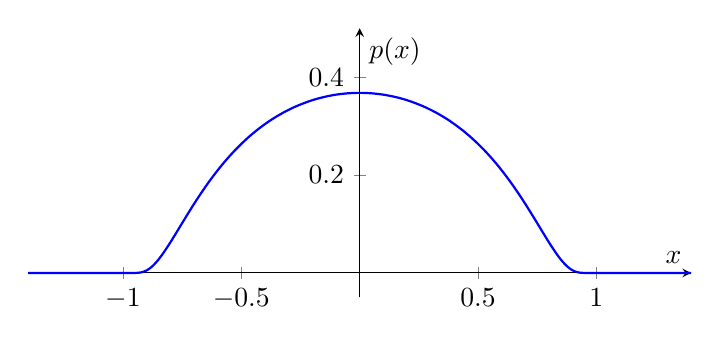
\begin{tikzpicture}
\begin{axis}[
    width=10cm, height=5cm,
    axis lines=middle,
    xlabel={$x$}, ylabel={$p(x)$},
    xmin=-1.4, xmax=1.4,
    ymin=-0.05, ymax=0.5,
    samples=300,
    domain=-1.4:1.4
]
\addplot[thick, blue]
    {abs(x)<1 ? exp(-1/(1-x^2)) : 0};
\end{axis}
\end{tikzpicture}

Let $p_\epsilon (x) := \epsilon^{-d} p(\frac{x}{\epsilon})$. Then
\[
    \int p_\epsilon(x) \; dx = \epsilon^{-d}\int p(\frac{x}{\epsilon}) \; dx
\]  
By change of variable $x' = \frac{x}{\epsilon}$, $dx' = \frac{dx}{\epsilon^d}$,
\[
    = \epsilon^{-d} \int_{\R^d} p(x') \epsilon^d \; dx' = \int_{\R^d} p(x') \; dx' = 1
\] 
And $p_\epsilon$ is supported on $B(0, \epsilon)$.

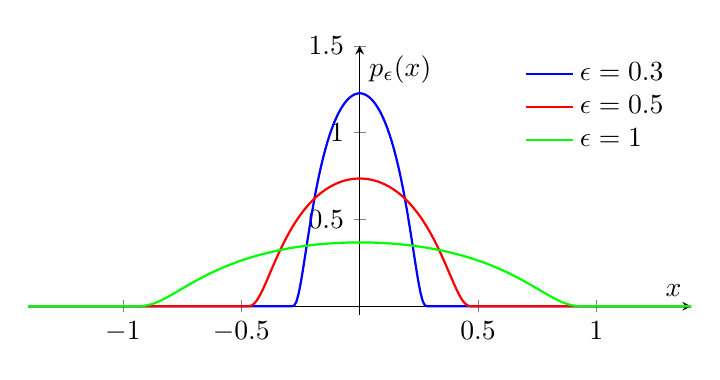
\begin{tikzpicture}
\begin{axis}[
    width=10cm, height=5cm,
    axis lines=middle,
    xlabel={$x$}, ylabel={$p_\epsilon(x)$},
    xmin=-1.4, xmax=1.4,
    ymin=-0.05, ymax=1.5,
    samples=300,
    domain=-1.4:1.4,
    legend style={at={(0.98,0.98)}, anchor=north east, draw=none, fill=none},
    legend cell align=left
]
\addplot[thick, blue]
    {abs(x/0.3)<1 ? (1/0.3)*(exp(-1/(1-(x/0.3)^2))) : 0};
\addlegendentry{$\epsilon=0.3$}

\addplot[thick, red]
    {abs(x/0.5)<1 ? (1/0.5)*(exp(-1/(1-(x/0.5)^2))) : 0};
\addlegendentry{$\epsilon=0.5$}

\addplot[thick, green]
    {abs(x)<1 ? exp(-1/(1-x^2)) : 0};
\addlegendentry{$\epsilon=1$}
\end{axis}
\end{tikzpicture}

$\{p_{\epsilon}\}_{\epsilon>0} $ is a family of "kernels" which belong to:

\begin{defn}[good kernel]
    Let $\{K_\epsilon\}_{\epsilon > 0}$ be a collection of functions s.t. $K_\epsilon : \R^d \to \R$ satisfies:
    \begin{enumerate}
        \item $\int_{\R^d} K_\epsilon(x) \; dx = 1$ for all $\epsilon > 0$
        \item $K_\epsilon \in L^1(\R^d)$ for all $\epsilon > 0$
        \item $\forall \delta > 0$, $\int_{|x| > \delta} |K_\epsilon(x)| \; dx \to 0$ as $\epsilon \to 0$. 
    \end{enumerate}  
    Then we call $\{K_\epsilon\}_{\epsilon > 0}$ a set of \newword{good kernels}. We call these kernels 
    because we will typically consider 
    \[
        f_\epsilon(x) := p_\epsilon * f = \int f(x-y)\underbrace{p_\epsilon(y) \; dy}_{\text{conv. kernel}}
    \] 
    Since $p_\epsilon \in C_c^{\infty}(\R^d)$, $\forall f \in L^p|\R^d|$, $f_\epsilon \in C^\infty(\R^d)$, 
    so $f_\epsilon$ is "smoothing $f$ out".  
\end{defn}

\begin{thm}[approximation using mollifiers]
    Let $p_\epsilon, f_\epsilon$ be as above. Then
    \begin{enumerate}
        \item If $f \in L^\infty(\R^d)$, and $f$ is continuous at $x$, then $f_\epsilon(x) \xrightarrow[\epsilon \to 0]{} f(x)$
            i.e. $f_\epsilon$ converges pointwise to $f$ at the continuity points of $f$;
            \item If $f \in C(\R^d)$, $f_\epsilon \xrightarrow[\epsilon \to 0]{} f$ uniformly on compact sets;
            \item If $f \in L^p(\R^d)$, then $f_\epsilon \xrightarrow[\epsilon \to 0]{} f$ in $L^p(\R^d)$      
    \end{enumerate} 
\end{thm}
\begin{rem}
    This is true for all good kernels $\{K_\epsilon\}_{\epsilon > 0}$ s.t. $f_\epsilon$ is well defined.
    But it is easier to redo the proof later than store a general result.
\end{rem}
\begin{proof} \leavevmode
    \begin{description}
        \item[(1)] $f$ continuous on $x$ therefore $\forall \eta > 0$, $\exists \delta > 0$
        s.t. $|x - y| < \delta \Rightarrow |f(x) - f(y)| < \eta$. So 
        \begin{align*}
            |f_\epsilon(x) - f(x)| &= \left| \int f(x-y) p_\epsilon(y) \; dy  - f(x) \right| \\
            &= \left| \int f(x-y) p_\epsilon(y) \; dy - \int f(x) p_\epsilon (y) \; dy \right| \\
            &= \left| \int (f(x-y) - f(x)) p_\epsilon \; dy \right|  \\  
            &\leq \int_{|y| \leq \delta} |f(x-y) - f(x)| p_\epsilon(y) \; dy +
            \int_{|y| > \delta} (|f(x-y)| - |f(y)|) p_\epsilon(y) \; dy \\
            &\leq \eta \int_{\R^d} p_\epsilon(y) \; dy + 2 \| f \|_\infty \int_{|y| > \delta} p_\epsilon(y) \; dy \\
            &= \eta + 2 \| f \|_\infty \int_{|y| > \delta \cap |y| < \epsilon} p_\epsilon(y) \; dy \\
        \end{align*}    
        If $\epsilon < \delta$, then $\supp(p_\epsilon) \subseteq B(0, \delta)$ so
        $\int_{|y| > \delta \cap |y| < \epsilon} p_\epsilon(y) \; dy \to 0$ as $\epsilon \to 0$,
        and thus
        \[
            \lim_{\epsilon \to 0} |f_\epsilon(x) - f(x)| \leq \eta \quad \forall \eta > 0
            \Rightarrow \lim_{\epsilon \to 0} |f_\epsilon(x) - f(x)| = 0
        \] 
        \item[(2)] If $f \in C(\R^d)$, then fix $K \subseteq \R^d $ compact. Therefore
        $f$ is uniformly continuous on $K$. So $\forall \eta > 0$, $\exists \delta > 0$ s.t.
        $|x - y| < \delta \Rightarrow \sup_{x \in K} |f(x) - f(y)| < \eta$.
        
        Also, $f \in C(\R^d)$ so 
        \[
            \frac{\sup}{K + B(0, 1)} |f(z)| \leq C
        \]
        So
        \begin{align*}
            |f_\epsilon(x) - f(x)| &\leq \int_{|y| < \delta} |f(x-y) - f(x)| p_\epsilon(y) \; dy + \int_{|y| > \delta} (|f(x-y)| + |f(x)|) p_\epsilon(y) \; dy \\
            &\leq \sup_{x \in K} \int_{|y| < \delta} |f(x-y) - f(x)| p_\epsilon(y) \; dy + \sup_{x \in K} \int_{|y| > \delta \cap |y| \leq \epsilon} (|f(x-y)| + |f(x)|) p_\epsilon(y) \; dy \\
            &\leq \eta + \frac{\sup}{K + B(0, 1)} |f(z)| \int_{|y| > \delta \cap |y| \leq \epsilon} p_\epsilon(y) \; dy \\
        \end{align*}      
        Therefore 
        \[
        \lim_{\epsilon \to 0} \sup_{x \in K} |f_\epsilon(x) - f(x)| \leq \eta \quad \forall \eta > 0 
        \]
        And thus $f_\epsilon \to f$ uniformly on $K$.   
        \item[(3)] If $f \in L^p(\R^d)$, then $\forall \eta > 0$, $\exists \tilde{f} \in C_c(\R^d)$
        s.t. 
        \[
        \| f - \tilde{f} \|_p < \eta
        \]  
        Since $\tilde{f} \in C_c(\R^d)$, $p_\epsilon$ is compactly supported, $\tilde{f_\epsilon} \in C_c^\infty(\R^d)$
        is compactly supported, so $\tilde{f_\epsilon} \to \tilde{f}$ uniformly on $\R^d$. Also,
        since $\tilde{f_\epsilon}, \tilde{f}$ are compactly supported, 
        \[
            \int |\tilde{f_\epsilon} - \tilde{f}|^p \; dx = \int_A |\tilde{f_\epsilon} - \tilde{f}|^p \; dx \leq \underbrace{\| \tilde{f_\epsilon} - \tilde{f} \|_\infty}_{\to 0 \text{ as } \epsilon \to 0} |A| 
        \]       
        Therefore $\tilde{f_\epsilon} \to \tilde{f}$ in $L^p(\R^d)$. Thus,
        \begin{align*}
            \| f_\epsilon - f \|_p &\leq \| f_\epsilon - \tilde{f_\epsilon} \|_p + \| \tilde{f_\epsilon} - \tilde{f} \|_p + \| \tilde{f} - f \|_p \\    
            &= \| (f - \tilde{f}) * p_\epsilon \|_p + \| \tilde{f_\epsilon}  - \tilde{f}\|_p + \| \tilde{f} - f \|_p \\
            &\leq \| f - \tilde{f} \|_p \| p_\epsilon \|_1 + \| \tilde{f_\epsilon} - \tilde{f} \|_p + \| \tilde{f} - f \|_p \\
            &\leq 2 \eta + \| \tilde{f_\epsilon} - \tilde{f} \|_p     
        \end{align*}  
        So, $\forall \eta > 0$,
        \[
            \lim_{\epsilon \to 0} \| f_\epsilon - f\|_p \leq 2 \eta \quad \Rightarrow f_\epsilon \to f \text{ in } L^p(\R^d) \qedhere 
        \]  
    \end{description}
\end{proof}

\begin{cor}
    $C_c^\infty(\R^d)$ is dense in $L^p(\R^d)$
\end{cor}
\begin{proof}
    By prior estimate, $\tilde{f_\epsilon} \in C_c^\infty{\R^d}$ and $\{\tilde{f_\epsilon}\}_{\epsilon > 0}$
    are dense in $L^p(\R^d)$. \qedhere   
\end{proof}

\begin{thm}[Weierstrass Approximation Theorem]
    Let $[a, b] \subseteq \R$, $f \in C([a,b])$. Then $\forall \eta > 0$, $\exists$ a polynomial
    $P$ s.t. 
    \[
        \sup_{x \in [a,b]} |f(x) - P(x)| < \eta
    \]      
    i.e. polynomials are dense in $(C([a,b]), \|\cdot\|_\infty)$.
\end{thm}
\begin{proof}
    We use a good kernel. First, for $f \in C([a,b])$, extend to $f \in C_c(\R)$.  \footnote{e.g. by linear interpolation}  
    Consider 
    \[
        K_\epsilon(x) = \frac{1}{\sqrt{\epsilon}}e^{-\frac{\pi x^2}{\epsilon}}
    \] 
    \textbf{Claim:} $\{K_\epsilon\}_{\epsilon > 0}$ is a family of good kernels.
    \newline \noindent Recall that
    \[
        \frac{1}{\sqrt{2\pi}} \int_{-\infty}^\infty e^{-\frac{x^2}{2}} \; dx = 1
    \] 
    We check:
    \begin{align*}
        \int K_\epsilon(x) \; dx &= \int \frac{1}{\sqrt{\epsilon}}e^{-\frac{\pi x^2}{\epsilon}} \; dx \\
        y = \frac{\sqrt{2\pi}}{\sqrt{\epsilon}}x &\Rightarrow dy = \frac{\sqrt{2\pi}}{\sqrt{\epsilon}}dx \\
        &= \int \frac{1}{\sqrt{\epsilon}} \frac{\sqrt{\epsilon}}{\sqrt{2\pi}} e^{-\frac{y^2}{2}} \; dy  = 1\\
    \end{align*}
    Also, 
    \[
        \int |K_\epsilon(x)| \; dx = \int K_\epsilon(x) \; dx = 1
    \] 
    Finally, we check $\forall \delta > 0$,
    \begin{align*}
        \int_{|x| > \delta} |K_\epsilon(x)| \; dx &= \int_{|x| > \delta} \frac{1}{\sqrt{\epsilon}} e^{-\frac{\pi x^2}{\epsilon}} \; dx \\
        &= \int_{|y| > \frac{\sqrt{2\pi}}{\sqrt{\epsilon}} \delta} \frac{1}{\sqrt{2\pi}} e^{-\frac{y^2}{2}} \; dy \\
        &\leq \int_{|y| \geq \frac{\sqrt{2\pi}}{\sqrt{\epsilon}} \delta} \frac{1}{\sqrt{2\pi}} |y| e^{-\frac{y^2}{2}} \; dy \\
        &= 2 \int_{\frac{\sqrt{2\pi}}{\sqrt{\epsilon}} \delta}^{\infty} \frac{1}{\sqrt{2 \pi}} r e^{-\frac{r^2}{2}} \; dr \\
        &= C e^{\frac{-r^2}{2}} \Big|_{\frac{\sqrt{2\pi}}{\sqrt{\epsilon}} \delta}^{\infty} \xrightarrow{\epsilon \to 0} 0 \\
    \end{align*}
    So $\{K_\epsilon\}$ are good kernels. Although $K_\epsilon$ is not compactly supported, 
    $f$ is compactly supported, so the same argument as in thm gives
    \[
        (f * K_\epsilon) \xrightarrow{\epsilon \to 0} f \quad \text{uniformly on } [a,b]
    \]   
    So $\exists \epsilon_0 > 0$ fixed s.t.
    \[
        \| f * K_{\epsilon_0} - f \|_{L^\infty([a,b])} < \frac{\eta}{2} \quad (*)
    \]  
    \textbf{Claim:} $\exists$ polynomial $P_N$ (of degrees $N$) s.t. $\|P_N - (f * K_{\epsilon_0})\|_{L^\infty([a,b])} < \frac{\eta}{2}$.  
    \newline \noindent Recall
    \[
        e^y = \sum_{n = 0}^\infty \frac{y^n}{n!}
    \] 
    which converges uniformly on compact sets. Define $M > 0$ s.t. 
    \[
        \sup_{x \in [a,b]} \sup_{y \in [-M, M]} |x-y| \leq M
    \]  
    So $\exists N$ s.t.
     \[
        \left\| K_{\epsilon_0}(x) - \underbrace{\frac{1}{\sqrt{\epsilon_0}} \sum_{n = 0}^N \frac{(-\frac{\pi x^2}{\epsilon_0})^n}{n!}}_{=: S_N(x)} \right\|_{L^\infty([-M, M])} < \frac{\eta}{4 M \| f \|_\infty} \footnote{Note, $S_N$ is a polynomial}
     \] 
    So $\forall x \in [a,b]$,
    \begin{align*}
        |f*K_{\epsilon_0}(x) - f*S_N(x)| &\leq \left| \int_{\R} f(x-y)(K_{\epsilon_0}(y) - S_N(y)) \; dy \right| \\
        &\leq \int_{-M}^M |f(x-y)| \left| |K_{\epsilon_0}(y) - S_N(y) \right| \; dy \\
        &\leq \| f \|_\infty \frac{\eta}{4 M \| f \|_\infty } 2M = \frac{\eta}{2}  
    \end{align*} 
    Finally, $S_N$ is a polynomial, so
    \[
        P_N(x) := (f* S_N)(x) = \int_{\R} f(y) S_N(x-y) \; dy \quad \text{ is a polynomial in } x
    \]  
    So $\forall \eta > 0$,
    \[
        \| P_N - f \|_{L^\infty([a,b])} \leq \| P_N - f * K_{\epsilon_0} \|_{L^\infty([a,b])} + \| f * K_{\epsilon_0} - f \|_{L^\infty([a,b])} < \frac{\eta}{2} + \frac{\eta}{2} = \eta \qedhere
    \]  
\end{proof}
\section{A Taste of Fourier}
\subsection{Fourier Series}

Fourier analysis for a complex function $f$ that is periodic. We let the torus 
$\mathbb{T} = [0, 1) \sim \R / \Z$ and we consider 
\[
    L^2(\mathbb{T}; \C) = \left\{ f : \mathbb{T} \to \C : \int_0^1 |f(x)|^2 dx < \infty \right\} 
    \footnote{Note $|f| = \sqrt{\real(f)^2 + \imag(f)^2}$ }
\] 
Now, $f : \mathbb{T} \to \C$ is the same as $\tilde{f} : \R \to \C$ with $\tilde{f}$
being 1-periodic. We will build an inner product
$(. , .) : L^2(\mathbb{T}; \C) \times L^2(\mathbb{T}; \C) \to \C$.

\begin{defn}[complex inner product]
    A \newword{complex inner product} on a complex vector space $V$ is a function $(. , .) : V \times V \to \C$ 
    such that for all $u, v, w \in V$ and $\alpha \in \C$, we have
    \begin{enumerate}
         \item $(\alpha u + v, w) = \alpha (u, w) + (v, w)$
        \item $(u, v) = \overline{(v, u)}$
        \item $(u, u) \geq 0$ and $(u, u) = 0$ if and only if $u = 0$
    \end{enumerate}
\end{defn}

\begin{prop}
    \[
        (f, g) := \int_0^1 f(x) \overline{g(x)} \; dx
    \] 
    defines a complex inner product on $L^2(\mathbb{T}; \C)$.
\end{prop}
\begin{proof} \leavevmode
    \begin{description}
        \item[(1)] Let $\alpha \in \C$. Then
        \[
            (\alpha f + h, g) = \int_0^1 (\alpha f(x) + h(x)) \overline{g(x)} \; dx = \alpha (f, g) + (h, g)
        \]  
        \item[(2)] 
        \begin{align*}
            (f, g) = \int_0^1 f(x) \overline{g(x)} \; dx &= \int_0^1 (\real f + i \imag f)(\real g - i \imag g) \; dx \\
            &= (a + bi) (c - di) \\
            &= (ac + bd) + i (bc - ad) \\
            &= \overline{(ac + bd) + i (ad - bc)} \\
            &= \overline{(a-bi) (c + di)} \\
            &= \overline{\int_0^1 \overline{(\real f + i \imag f)} (\real g + i \imag g) \; dx} \\
            &= \overline{(g, f)}
        \end{align*}
        \item[(3)] 
        \[
            (f, f) = \int_0^1 f(x) \overline{f(x)} \; dx = \int_0^1 |f(x)|^2 \; dx \geq 0  
        \] 
        Thus $(f, f) = \| f \|_{L^2(\mathbb{T}; \C)}^2 $ and $(f, f) = 0 $ iff $|f| = 0$ for 
        a.e. $x$ iff $f = 0$ in $L^2(\mathbb{T}; \C)$. \qedhere   
    \end{description}
\end{proof}

\begin{rem}
    $f \in L^2(\mathbb{T}; \C) \longleftrightarrow \real (f), \imag (f) \in L^2(\mathbb{T}; \R)$.
    So $\{f_n \}$ is Cauchy in $L^2(\mathbb{T}; \C)$ iff 
$\{ \real (f_n) \}_{n=1}^\infty$ and $\{ \imag (f_n) \}_{n=1}^\infty$ are Cauchy in $L^2(\mathbb{T}; \R)$.

Also, we know $L^2(\mathbb{T}; \R)$ is complete, so $L^2(\mathbb{T}; \C)$ is a Hilbert space.   
\end{rem}
\begin{rem}
    We still have Cauchy Schwartz, i.e. 
    \[
        |(f, g)| \leq \| f \| \| g \|  
    \] 
\end{rem}

\begin{thm}
    Let $e_n(x) := e^{2 \pi i n x} = \cos(2 \pi n x) + i \sin(2 \pi n x)$. Then
    $\{e_{n}(x)\}_{n \in \Z}$ is an orthonormal basis for $L^2(\mathbb{T}; \C)$. 
\end{thm}
\begin{proof}
    Observe 
    \[
        (e_n, e_m) = \int_0^1 e^{2 \pi i n x} e^{-2 \pi i m x} \; dx = \int_0^1 e^{2 \pi i (n - m) x} \; dx
    \] 
    If $n = m$, then $\int_0^1 e^0 \; dx  = 1$, therefore $\| e_n \| = 1 \; \forall n$.

    If $n \neq m$, then 
    \[
    \int_0^1 e^{2 \pi i (n - m) x} \; dx  = \frac{1}{2 \pi i (n - m)} e^{2 \pi i (n - m)x} \Big|_0^1 = \frac{1}{2 \pi i (n - m)} (e^{2 \pi i (n - m)} - 1)
    \]
    But $e^{2 \pi i (n - m)} = \underbrace{\cos(2 \pi (n - m))}_{= 1} + i \underbrace{\sin(2 \pi (n - m))}_{= 0} = 1$.
    
    So $\int_0^1 e^{2 \pi i (n - m) x} \; dx = 0$. Thus $\{e_n\}_{n \in \Z}$ is orthonormal.
    \newline \textbf{Claim:} $\{e_n\}_{n \in \Z}$ is a basis of $L^2(\mathbb{T}; \C)$, i.e. 
    $\forall f \in L^2(\mathbb{T}; \C)$, $\exists \{\alpha_n \}_{n \in \Z} \subseteq \C$ s.t.
    \[
        f = \sum_{n=-\infty}^\infty \alpha_n e_n = \lim_{N \to \infty} \sum_{n=-N}^N \alpha_n e_n
    \]   
    To prove the claim we use complex Stone-Weierstrass. Let
    \[
        \mathcal{A} = \left\{ \sum_{n = -N}^N \alpha_n e_n : \alpha_n \in \C \right\} 
    \] 
    We need that $\mathcal{A}$ is an algebra, which is clear since $e_n e_m = e^{2 \pi i (n + m) x} = e_{n+m}$.
    We also need that $\mathcal{A}$ contains constants, which is clear since $e_0 = 1$. We also
    need that $\mathcal{A}$ is closed under conjugates, which is also clear because $\overline{\alpha_n} \in \C$,
    $\overline{e_n} = e_{-n}$. Finally, we need that $\mathcal{A}$ separates points. 
    If $x \neq y$, $x, y \in [0, 1)$, then $\forall n$ s.t. $nx - ny \notin \Z$, we have
    \[
        e_n(x) = e^{2 \pi i n x} \neq e^{2 \pi i n y} = e_n(y)
    \]
    So $\mathcal{A}$ separates points. 
    
    Thus by complex Stone-Weierstrass, since $\mathbb{T}$ is compact, $\mathcal{A}$ is dense in $C(\mathbb{T}; \C)$
    so $\forall \tilde{f} \in C(\mathbb{T}; \C)$, 
    \[
        \tilde{f} = \lim_{N \to \infty} \sum_{n=-N}^N \alpha_n e_n \quad \text{ limit in }  \| . \|_\infty
    \] 
    Since $\| . \|_\infty \geq \| . \|_{L^2}$, we also have $\tilde{f} = \lim_{N \to \infty} \sum_{n=-N}^N \alpha_n e_n$ in $\| . \|_{L^2}$.
    Finally, we know $C(\mathbb{T}; \C)$ is dense in $L^2(\mathbb{T}; \C)$.
    Therefore $\forall \eta > 0$,
    \[
        \lim_{N \to \infty} \| f - \sum_{n = -N}^N \alpha_n e_n \|_{2} \leq \| f - \tilde{f} \|_2 + 
        \| \tilde{f} - \sum_{n = -N}^N \alpha_n e_n \|_2 \leq \eta + 0 = \eta  
    \]  
    Therefore $f = \sum_{n = -\infty}^\infty \alpha_n e_n$ in $L^2(\mathbb{T}; \C)$, as desired. \qedhere 

\end{proof}

\begin{rem}
    Recall that TFAE:
    \begin{enumerate}
        \item $\{e_n\}_{n \in \Z}$ is a basis 
        \item Every $f \in L^2(\mathbb{T}; \C)$, $f = \sum_{n = -\infty}^\infty \alpha_n e_n = \sum_{n=-\infty}^\infty (f, e_n) e_n$
        \item Completeness: If $(f, e_n) = 0$ for all $n$, then $f = 0$
        \item Parseval: $\| f \|_2^2 = \sum_{n=-\infty}^\infty |(f, e_n)|^2 $  
    \end{enumerate}
\end{rem}

\begin{defn}[Fourier Series]
    For $n \in \Z$, let
    \[
        \hat{f}(n) := (f, e_n) = \int_0^1 f(x) e^{-2 \pi i n x} \; dx
    \]  
    Then the (complex) \newword{Fourier series} of $f : \mathbb{T} \to \C$ is defined by
    \[
        \sum_{n = -\infty}^\infty \hat{f}(n)e^{2 \pi i n x}
    \] 
\end{defn}

\begin{rem}
    It is possible to define a Fourier series for any periodic function. If $f$ is $L-$periodic,
    then 
    \[
        \hat{f}_L(n) := \frac{1}{L} \int_0^L f(x) e^{-2 \pi i n x / L} \; dx
    \]   
    Therefore we get the Fourier series
    \[
        \sum_{n = -\infty}^\infty \hat{f}_L(n) e^{2 \pi i n x / L}
    \] 
\end{rem}
\begin{rem}
    It is also possible to define a real valued Fourier series, using sines and cosines.
    \[
        A_0 + \sum_{n = 1}^\infty A_n \cos(\frac{2 \pi n x}{L}) + B_n \sin(\frac{2 \pi n x}{L})
    \] 
    for some some $A_n, B_n$, also given by inner products.  
\end{rem}

\begin{goal}[question]
    In what sense does 
    \[
        \sum_{n = -\infty}^\infty \hat{f}(n) e^{2 \pi i n x} = \lim_{N \to \infty} \sum_{n = -N}^N \hat{f}(n) e^{2 \pi i n x} =: \lim_{N \to \infty} S_N(x)
    \] 
    converge?
\end{goal}

\begin{prop}
    If $f \in L^2(\mathbb{T}; \C)$, then
    \[
        f(x) = \lim_{N \to \infty} S_N(x) \text{ in } L^2(\mathbb{T}; \C)
    \]  
\end{prop}
\begin{proof}
    Immediate from the basis \qedhere
\end{proof}

Observe that by Parseval, we have 
\[
    \| f \|_2^2 = \sum_{n = -N}^N |(f, e_n)|^2 = \sum_{n=-\infty}^\infty |\hat{f}(n)|^2
\] 
Therefore $\lim_{n \to \infty} |\hat{f}(n)|^2 = 0 \iff \lim_{n \to \infty} |\hat{f}(n)| = 0$. 
\footnote{Can also be seen using Bessel's inequality, $\sum_{n = -\infty}^\infty |\hat{f}(n)|^2 \leq \| f \|_2^2$ }
This gives us

\begin{prop}[Riemann-Lebesque Lemma]
    If $f \in L^2(\mathbb{T}; \C)$, then $\lim_{n \to \infty} |\hat{f}(n)| = 0$.
\end{prop}

\begin{rem}
    This is very useful for the "real Fourier series" version,
    \[
        \lim_{n \to \infty} \int_0^1 f(x) \sin(2 \pi n x) \; dx = \lim_{n \to \infty} \int_0^1 f(x) \cos(2 \pi n x) \; dx = 0
    \] "Oscillatory integrals" (important in PDEs).
\end{rem}

What about other notions of convergence?
\begin{align*}
    S_N(x) &= \sum_{n=-N}^N \hat{f}(n) e^{2 \pi i n x} \\
    &= \sum_{n = -N}^N \left( \int_0^1 f(y) e^{-2 \pi i n y} \; dy \right) e^{2 \pi i n x} \\
    &= \int_0^1 f(y) \left( \sum_{n = -N}^N e^{2 \pi i n (x - y)} \right) dy
\end{align*}
Let $D_N(x) := \sum_{n = -N}^N e^{2 \pi i n x}$. $D_N$ is called the \newword{Dirichlet kernel}.
\[
    S_N(x) = \int_0^1 f(y) D_N(x - y) \; dy = (f * D_N)(x) \quad \text{ "convolution on the torus"}
\] 

\underline{Observe:}
\[
    D_N(x) = 1 + \sum_{n = 1}^N \underbrace{e^{2 \pi i n x}}_{1-periodic} - \underbrace{e^{-2 \pi i n x}}_{\text{1-periodic}}
\]  
Therefore $D_N$ is 1-periodic, and
\[
    \int_0^1 D_N(x) \; dx = \int_0^1 1 + (\text{1-periodic}) \; dx = 1
\]  

\begin{rem}
    $D_N$ is NOT a good kernel. In particular, 
    \[
        \int_0^1 |D_N(x)| \; dx \geq C \log N \to \infty \text{ as } N \to \infty
    \]  
    However, we can rewrite $D_N$ as
    \begin{align*}
        D_N(x) = \sum_{n = -N}^N e^{2 \pi i n x}  &= \sum_{n = -N}^N \left(e^{2 \pi i x}\right)^n\\
        &= \sum_{n = 0}^{2N} e^{2 \pi i x (n - N)} \\
        &= e^{-2 \pi i N x} \underbrace{\sum_{n = 0}^{2N} \left(e^{2 \pi i x}\right)^n}_{\text{finite geometric series}} \\
        &= e^{-2 \pi i N x} \frac{1 - e^{2 \pi i x (2N + 1)}}{1 - e^{2 \pi i x}} \\
        &= \frac{e^{-2 \pi i N x} - e^{2 \pi i x (N + 1)}}{1 - e^{2 \pi i x}} \\
        &= \frac{e^{-2 \pi i x \cdot \frac{1}{2}} \left( e^{-2 \pi i N x } - e^{2 \pi i (N + 1) x } \right)}{e^{-2 \pi i x \cdot \frac{1}{2}}\left(1 - e^{2 \pi i x}\right)} \\
        &= \frac{e^{-2 \pi i (N + \frac{1}{2}) x} - e^{-2 \pi i (N + \frac{1}{2}) x}}{e^{-2 \pi i \frac{1}{2} x} - e^{2 \pi i \frac{1}{2} x}} \\
        &= \frac{\sin(2 \pi (N + \frac{1}{2} )x)}{\sin(\pi x)}
    \end{align*}
    So $D_N$ is a "rescaled sine function". The sine function is a good kernel, but the rescaling is bad.
    Using this representation, we have the following theorem.
\end{rem}

\begin{thm}[pointwise convergence]
    Let $f \in L^2(\mathbb{T}; \C)$, and $f$ is Lipschitz continuous at $x_0$. Then
    \[
        S_N f(x_0) \to f(x_0) \text{ as } N \to \infty
    \]   
\end{thm}
\begin{proof}
    Proof on the assignment
\end{proof}
\begin{thm}[uniform convergence]
    If $f \in C^2(\mathbb{T}; \C)$ then $S_N f (x) \to f(x)$  on $\mathbb{T}$.   
\end{thm}
\begin{proof}
    Proof on the assignment.
\end{proof}

\begin{rem}
    In fact, we see
    \[
        \hat{f}(n) = \int_0^1 f(x) e^{-2 \pi i n x} \; dx
    \]
    is well defined whenever $f \in L^1(\mathbb{T}; \C)$. \footnote{Since $|e^{-2 \pi i n x}| = 1$}
    Therefore many Fourier things will be good for $L^1(\mathbb{T}; \C)$, not just $L^2(\mathbb{T}; \C)$. 
\end{rem}

\subsection{The Fourier Transform}
Last class, we had $\hat{f} = (f, e_n) = \int_0^1 f(x) e^{-2 \pi i n x} \; dx$ 
are the fourier coefficients for $f : \mathbb{T} \to \C$, and this quanity is finite $\forall
f \in L^1(\mathbb{T}; \C)$, $L^2(\mathbb{T}; \C) \subseteq L^1(\mathbb{T}; \C)$. We now introduce:

\begin{defn}[Fourier Transform]
    Let $f : \R \to \C$. Then $\forall \zeta \in \R$,
    \[
        \hat{f}(\zeta) := \int_{\R} f(x) e^{-2 \pi i \zeta x} \; dx
    \]   
\end{defn}

\begin{rem}
    We will reserve $x, y, z$ for variables in the physical space, and $\zeta, \eta, \xi$ for
    variables in the "Fourier space".  
\end{rem}

\begin{prop}
    If $f \in L^1(\R; \C)$, then $\hat{f} \in L^\infty(\R; \C) \cap C(\R; \C)$. 
    \footnote{We will drop the $\C$ from now on, but everything can be complex valued. }
\end{prop}
\begin{proof}
    We have
    \begin{align*}
        |\hat{f}(\xi)| = \left| \int_{\R} f(x) e^{-2 \pi i \xi x} \; dx \right| \leq 
        \int_{\R} |f(x)| |e^{-2 \pi i \xi x}| \; dx = \int_{\R} |f(x)| \; dx = \| f \|_1
    \end{align*}
    Therefore $\| \hat{f} \|_\infty \leq \| f \|_1 $.

    Moreover, $\forall h > 0$,
    \begin{align*}
        |\hat{f}(\zeta + h) - \hat{f}(\zeta)| &= \left| \int_{\R} f(x) e^{-2 \pi i (\zeta + h) x} \; dx - \int_{\R} f(x) e^{-2 \pi i \zeta x} \; dx \right| \\
        &= \left| \int_{\R} f(x) e^{-2 \pi i \zeta x}(e^{-2 \pi i h x} - 1) \; dx \right| \\
        &\leq \int_{\R} |f(x)| \underbrace{|e^{-2 \pi i \zeta x}|}_{=1} |e^{-2 \pi i h x} - 1| \; dx
    \end{align*}
    Also, $\lim_{h \to 0} |e^{-2 \pi i h x} - 1| = 0$, $\forall x \in \R$ and
    \[
        |f(x)| |e^{-2 \pi i h x} - 1| \leq |f(x)|(|e^{-2 \pi i h x}| + 1) = 2 |f(x)| \in L^1(\R)
    \]  
    Therefore by DCT,
    \[
        \lim_{h \to 0} |\hat{f}(\zeta + h) - \hat{f}(\zeta)| = \int_{\R} |f(x)| \underbrace{\lim_{h \to 0} |e^{-2 \pi i h x} - 1|}_{=0} \; dx = 0 \qedhere
    \] 
\end{proof}

\begin{prop}
    Let $f,g \in L^1(\R)$. Then
    \begin{enumerate}
        \item $\widehat{f*g} = \hat{f} \cdot \hat{g}$;
        \item $\int_{\R} f \hat{g} \; dx = \int_{\R} \hat{f} g \; dx$ 
    \end{enumerate} 
\end{prop}
\begin{proof} \leavevmode
    \begin{description}
        \item[(a)] 
        \[
            \widehat{f * g}(\zeta) = \int (f*g)(x) e^{-2 \pi i \zeta x} \; dx = \iint f(x-y) g(y) \; dy \; e^{-2 \pi i \zeta x} \; dx
        \]  
        Since $f, g \in L^1(\R)$, this integral is finite\footnote{b/c $\leq \| f \|_1 \| g \|_1$ } so 
        by Fubini,
        \[
            = \iint_{\R} f(x-y) e^{-2 \pi i \zeta (x-y)} \; dx \; g(y) e^{-2 \pi i \zeta y} \; dy
        \] 
        Using $z = x-y$, 
        \[
            = \int \left( \int_{\R} f(z) e^{-2 \pi i \zeta z} \; dz \right) g(y) e^{-2 \pi i \zeta y} \; dy
            = \hat{f}(\zeta) \int g(y) e^{-2 \pi i \zeta y} \; dy = \hat{f} \hat{g}
        \]  

        \item[(b)] 
        \begin{align*}
            \int f(x) \hat{g(x)} &= \int f(x) \int g(y) e^{-2 \pi i x y} \; dy \; dx \\
            &= \int g(y) \underbrace{\int f(x) e^{-2 \pi i x y} \; dx}_{\hat{f}(y)} \; dy \quad \text{by Fubini} \\ 
            &= \int \hat{f}(y) g(y) \; dy \qedhere \\
        \end{align*}
    \end{description}
\end{proof}

\begin{lem}
    Let $f(x) = e^{-\pi a x^2}$, $a > 0$. Then
    \[
        \hat{f}(\zeta) = \frac{1}{\sqrt{a}}e^{-\pi \zeta^2 / a}
    \]   
\end{lem}
\begin{proof}
    We compute 
    \begin{align*}
        \hat{f'}(\zeta) &= \int_{\R} f'(x) e^{-2 \pi i \zeta x} \; dx \\
        &= f(x) e^{-2 \pi i \zeta x} \Big|_{-\infty}^\infty - \int_{\R} f(x) (-2 \pi i \zeta) e^{-2 \pi i \zeta x} \; dx \quad \text{by IBP}\\
        &= e^{-\pi a x^2}e^{-2 \pi i \zeta x} \Big|_{-\infty}^\infty + 2 \pi i \zeta \int_{\R} f(x) e^{-2 \pi i \zeta x} \; dx \\
        &= 0 - 0 + 2 \pi i \zeta \hat{f}(\zeta)
    \end{align*}
    Therefore $\hat{f'}(\zeta) = 2 \pi i \zeta \hat{f}(\zeta)$
    
    Also, 
    \[
        \frac{d}{d\zeta} \hat{f}(\zeta) = \frac{d}{d \zeta} \left( \int_{\R} f(x) e^{-2 \pi i \zeta x} \; dx \right)
    \] 
    To differentiate under the integral, we need to check DCT.
    \[
        \left| f(x) \left( \frac{e^{-2 \pi i x (\zeta + h)} - e^{-2 \pi i x \zeta}}{h} \right) \right| \leq |f(x)| \left| \frac{d}{d \zeta} e^{-2 \pi i x \zeta} \right| \Big|_{\zeta = \zeta^*} 
    \] 
    where $\zeta^* \in [\zeta, \zeta + h]$. Then
    \begin{align*}
        = |f(x)| |-2 \pi i x| |e^{-2 \pi i x \zeta^*}| = 2 \pi |f(x)| |x| = 2 \pi |x| e^{-\pi a x^2} \in L^1(\R)
    \end{align*}
    By DCT, 
    \begin{align*}
        \frac{d}{d \zeta} \hat{f}(\zeta) &= \int_{\R} f(x) \frac{d}{d \zeta}(e^{-2 \pi i x \zeta}) \; dx \\
        &= \int_{\R} f(x) (-2 \pi i x) e^{-2 \pi i x \zeta} \; dx \\
        &= i \int_{\R} (-2 \pi x) e^{-\pi a x^2} e^{-2 \pi i x \zeta} \; dx \\
        &= \frac{i}{a} \int_{\R} (e^{-\pi a x^2})' e^{-2 \pi i x \zeta} \; dx \\
        &= \frac{i}{a} \underbrace{\int_{\R} f'(x) e^{-2 \pi i \zeta x} \; dx}_{\hat{f'}(\zeta)} \\
        &= \frac{1}{a} 2 \pi i \zeta \hat{f}(\zeta) \\
        &= -\frac{2 \pi \zeta}{a} \hat{f}(\zeta)
    \end{align*}
    Thus,
    \begin{align*}
        \frac{d}{d \zeta} (e^{\pi \zeta^2 / a} \hat{f}(\zeta)) &= e^{\pi \zeta^2 / a} \frac{d}{d \zeta} \hat{f}(\zeta) + \frac{d}{d \zeta}(e^{\pi \zeta^2 / a}) \hat{f}(\zeta) = 0 \\
        &= \frac{-2 \pi \zeta}{a} e^{\pi \zeta^2 / a} \hat{f}(\zeta) + \frac{2 \pi \zeta}{a} e^{\pi \zeta^2/a} \hat{f}(\zeta) = 0
    \end{align*}
    So $\zeta \mapsto e^{\pi \zeta^2 / a} \hat{f}(\zeta)$ is constant in $\zeta$. Therefore
    \[
        e^{\pi \zeta^2/a} \hat{f}(\zeta) = e^{0} \hat{f}(0) = \hat{f}(0) = \int_{\R} e^{-\pi a x^2} \; dx = \frac{1}{\sqrt{a}} \int_{\R} e^{-\pi y^2} \; dy = \frac{1}{\sqrt{a}}
    \]  
    Therefore $\hat{f}(\zeta) = \frac{1}{\sqrt{a}} e^{-\pi \zeta^2 / a}$. \qedhere 
\end{proof}

\begin{defn}[Inverse Fourier Transform]
    If $f \in L^1(\R)$, then 
    \[
        \check{f}(x) := \int_{\R} f(\zeta) e^{2 \pi i x \zeta} d \zeta = \hat{f}(-x)
    \] 
\end{defn}
\begin{proof}
    If $f \in L^1(\R)$, then $\check{f} \in L^\infty(\R) \cap C(\R)$. The proof is identical to $\hat{f}$.   
\end{proof}

\begin{rem}
    We hope that if $f \in L^1(\R)$, then $\check{\hat{f}} = f$. However,
    \[
        \check{\hat{f}} = \int \left( \int f(z) e^{-2 \pi i \zeta z} \; dz \right) e^{2 \pi i x \zeta} \; d\zeta
        \leq \iint |f(z)| \; dz \; d \zeta = \infty
    \] 
\end{rem}
\begin{thm}[Fourier Inversion]
    If $f \in L^1(\R)$ and $\hat{f} \in L^1(\R)$, then $\exists f_0 \in C(\R)$ s.t. $f = f_0$ almost everywhere, and
    $f_0(x) = \hat{\check{f}} = \check{\hat{f}}.$ 
\end{thm}

\begin{rem}
    The inversion formula is an analog of convergence of Fourier series, because it says
    \[
        f(x) = \int \hat{f}(\zeta) e^{2 \pi i \zeta x} \; d\zeta \approx \sum_{\zeta \in \R} \hat{f}(\zeta) e^{2 \pi i \zeta x}
    \]  

\end{rem}

\begin{cor}
    If $ f \in L^1(\R)$, $\hat{f} \equiv 0 \Rightarrow f \equiv 0$ a.e. 
\end{cor}
\begin{proof}[Proof of Thm]
    Let $\epsilon > 0$. Fix $x \in \R$, and define $\phi^\epsilon(\zeta) = e^{2 \pi i x \zeta} e^{- \pi \epsilon \zeta^2}$ 
    Then
    \begin{align*}
        \hat{\phi^{\epsilon}}(y) &= \int \phi^{\epsilon}(\zeta) e^{-2 \pi i y \zeta} \; d \zeta \\
        &= \int e^{2 \pi i x \zeta} e^{- \pi \epsilon \zeta^2} e^{-2 \pi i y \zeta} \; d \zeta \\
        &= \int e^{- \pi \epsilon \zeta^2} e^{- 2 \pi i (y - x) \zeta} \; d \zeta \\
        &= \widehat{e^{-\pi \epsilon (.)^2}}(y - x) \\
        &= \frac{1}{\sqrt{\epsilon}} e^{-\pi (y - x)^2 / \epsilon} \quad \text{by lemma}\\
    \end{align*}   
    So 
    \[
        \int f \hat{\phi^\epsilon} \; dy = \int \hat{f} \phi^\epsilon \; dy
    \] 
    Therefore 
    \[
        \int f(y) \frac{1}{\sqrt{\epsilon}} e^{-\pi (x-y)^2 / \epsilon} \; dy = \int \hat{f}(y) \phi^\epsilon(y) \; dy
    \] 
    Let $K_\epsilon(y) := \frac{1}{\sqrt{\epsilon}} e^{-\pi y^2 / \epsilon}$. We saw that $\{ K_\epsilon\}$ are good kernels,
    so 
    \[
        \int \hat{f}(y) \phi^{\epsilon}(y) \; dy = (K_\epsilon * f)(x)
    \]   
    \textbf{Claim:} $K_\epsilon * f \to f$ in $L^1(\R)$.
    \newline \noindent If the claim holds, then
    \[
        f(x) = \lim_{\epsilon \to 0} \int \underbrace{\hat{f}(y) e^{2 \pi i x y} e^{- \pi \epsilon y^2}}_{\leq \|\hat{f}\|_{L^1}} \; dy
    \]  
    So by DCT,
    \[
        f(x) = \int \hat{f}(y) e^{2 \pi i x y} \; dy 
    \]  
    $f(x) = \check{\hat{f}}(x)$, therefore $f = \check{\hat{f}}$ a.e.
    An identical proof gives $f = \hat{\check{f}}$ a.e. Moreover, $\check{\hat{f}}$ and $\hat{\check{f}}$ are continuous,
    so $\exists f_0 \in C(\R)$ s.t. $f_0 = f$ a.e.
    \newline \noindent \textbf{Proof of claim:} 
    \newline \noindent \begin{align*}
        |(f * K_\epsilon)(x) - f(x)| &= \left| \int (f(x-y) - f(x)) K_\epsilon(y) \; dy \right| \\
        &\leq \int |f(x-y) - f(x)| K_\epsilon(y) \; dy \\ 
    \end{align*}
    Therefore
    \begin{align*}
        \int |(f * K_\epsilon)(x) - f(x)| \; dx &\leq \iint |f(x-y) - f(x)| K_\epsilon(y) \; dy \; dx \\
        &= \iint |f(x-y) - f(x) | \frac{1}{\sqrt{\epsilon}} e^{-\pi (y)^2 / \epsilon} \; dy \; dx \\
        &= \iint |f(x - \sqrt{\epsilon}y) - f(x)| \; dx \; e^{-\pi y^2} \; dy
    \end{align*} 
    Then by two DCT's, we can take $\epsilon \to 0$ inside the integral. (Finish proof in the posted notes)
\end{proof}

Let us introduce
\[
    C_0(\R) = \left\{ f \in C(\R) : \lim_{|x| \to \infty} |f(x)| = 0 \right\} \footnote{So $C_c(\R) \subseteq C_0(\R)$ }
\] 

\begin{prop}
    If $f \in C^1(\R) \cap C_0(\R) \cap L^1(\R)$ and $f' \in L^1(\R)$, then
    \[
        \widehat{f'}(\zeta) = (2 \pi i \zeta) \hat{f}(\zeta)
    \] 
    Additionally, if $f \in L^1(\R)$, then $\hat{f} \in C_0(\R)$. 
\end{prop}

\begin{proof}
    Identical to before. 
    \begin{align*}
        \widehat{f'}(\zeta) &= \int_{\R} f'(x) e^{-2 \pi i \zeta x} \; dx \\
        &= f(x) e^{-2 \pi i \zeta x} \Big|+{x = -\infty}^\infty - \int_{\R} f(x) (-2 \pi i \zeta) e^{-2 \pi i \zeta x} \; dx \\
        &= 0 - 0 + 2 \pi i \zeta \hat{f}(\zeta)
    \end{align*}
    For the second part, if $f \in L^1(\R)$, then $\exists \{f_n\} \subseteq C_c^\infty(\R)$ s.t. $\| f_n - f \|_1 \to 0$.
    Then $f_n' \in C_c(\R) \; \forall n$, therefore $f_n' \in L^1(\R)$. Therefore $\hat{f_n'} \in L^\infty(\R) \cap C(\R) \; \forall n$.
    So by the first claim,
    \[
        \hat{f_n'}(\zeta) = 2 \pi i \zeta \hat{f_n}(\zeta) \in L^\infty(\R) \cap C(\R) \; \forall n
    \]    
    Since $2 \pi i (.) \hat{f_n}(.) \in L^\infty(\R)$, we have
    \[
        |2 \pi i \zeta \hat{f_n}(\zeta)| \leq C, \Rightarrow |\zeta| |\hat{f_n}(\zeta)| \leq C \Rightarrow |\hat{f_n}(\zeta)| \leq \frac{C}{|\zeta|} \to 0 \text{ as } |\zeta| \to \infty
    \]  
    Therefore $\hat{f_n} \in C_0(\R), \; \forall n$.
    
    Moreover, since $\| f_n - f \|_1 \to 0 $, 
    \begin{align*}
        \| \hat{f_n} - \hat{f} \|_\infty &= \sup_{\zeta} \left| \int f_n(x) e^{-2 \pi i \zeta x} \; dx - \int f(x) e^{-2 \pi i \zeta x} \; dx \right| \\
        &= \sup_{\zeta} \left| \int (f_n(x) - f(x)) e^{-2 \pi i \zeta x} \; dx \right| \\
        &\leq \| f_n - f \|_1 \xrightarrow{n \to \infty} 0    
    \end{align*} 

    Finally, $\forall \zeta \in \R$,
    \[
        |\hat{f}(\zeta)| \leq |\hat{f_n}(\zeta)| + \| \hat{f_n} - \hat{f} \|_\infty 
    \]  
    Therefore
    \[
        \lim_{|\zeta| \to \infty} |\hat{f}(\zeta)| \leq \underbrace{\lim_{|\zeta| \to \infty} |\hat{f_n}(\zeta)|}_{0 \text{ bc } \hat{f_n} \in C_0(\R)} + \| \hat{f_n} - \hat{f} \|_\infty 
    \] 
    Taking $n \to \infty$,
    \[
        \lim_{|\zeta| \to \infty} |\hat{f}(\zeta)| = 0 \quad \Rightarrow \quad \hat{f} \in C_0(\R) \qedhere
    \]  
\end{proof}

\begin{rem}
    The second part of the proposition is the analogue of the Riemann-Lebesgue lemma except $f \in L^1(\R)$.
    \[
        \left[\lim_{n \to \infty} \int_0^1 f(x) e^{-2 \pi i n x} \; dx = 0 \right]
    \]      
\end{rem}

This gives us a good theory of Fourier Transforms for $f \in L^1(\R)$. However we would really like
to do it for $f \in L^2(\R)$ like before, and there's no easy way to compare $L^2(\R)$ and $L^1(\R)$.

\begin{thm}[Plancherel's Theorem]
    If $f \in L^1(\R) \cap L^2(\R)$, then $\hat{f} \in L^2(\R)$ and
    \[
        \| f \|_2 = \| \hat{f} \|_2 \quad \text{(isometry)}
    \]   
\end{thm}
\begin{rem}
    Recall Parseval's identity for Fourier series. 
    \[
        \| f \|_2^2 - \sum_{n \in \Z} |\hat{f_n}(n)|^2 \quad (\ell^2 \text{ version of Plancherel})
    \] 
\end{rem}
\begin{proof}
    Let $f \in L^1(\R) \cap L^2(\R)$. Let $g(x) := \overline{f(-x)}$. Then $g \in L^1(\R) \cap L^2(\R)$.
    Consider $\omega(x) := (f*g)(x)$. Then by Young's inequality,
    \[
        \| \omega \|_1 \leq \| f \|_1 \| g \|_1 \quad \Rightarrow \omega \in L^1(\R)
    \] 
    \textbf{Claim:} $\omega$ is continuous at $0$.
    \newline \noindent \begin{align*}
        |\omega(h) - \omega(0)| &= \left| \int f(h-y)g(y) \; dy - \int f(0 -y) g(y) \; dy \right| \\
        &= \left| \int (f(h-y) - f(-y))g(y) \; dy  \right| \\
        &\leq \| f(h - .) - f(.) \|_2 \| g \|_2 \\
        &= \| f(. - h) - f(.) \|_2 \| g \|_2 = \| \tau_h f - f \|_2 \| g \|_2        
    \end{align*}  
    Since $f \in L^2(\R)$, $\forall \eta > 0$, $\exists \tilde{f} \in C_c(\R)$ s.t. $\| \tilde{f} - f \|_2 < \eta$.
    Then,
    \[
        \| \tau_h f - f \|_2 \leq \underbrace{\| \tau_h f - \tau_h \tilde{f} \|_2}_{= \| f - \tilde{f} \|_2 } + \| \tau_h \tilde{f} - \tilde{f} \|_2 + \| \tilde{f} - f \|_2    
        \leq 2 \eta + \underbrace{\| \tau_h \tilde{f} - \tilde{f} \|_2}_{\tilde{f} \in C_c(\R)}
    \]    
    Therefore
    \[
        \| \tau_h \tilde{f} - \tilde{f} \|_\infty \xrightarrow{h \to 0} 0 \quad \Rightarrow \quad \| \tau_h \tilde{f} - \tilde{f} \|_2 \xrightarrow{h \to 0} 0 
    \] 
    So 
    \[
        \lim_{h \to 0} \| \tau_h f  - f \|_2 \leq 2 \eta \quad \forall \eta > 0 \quad \Rightarrow \quad \lim_{h \to 0} \| \tau_h f - f \|_2 = 0 
    \]  
    Thus $\lim_{h \to 0} |\omega(h) - \omega(0)| = 0$, and thus $\omega$ is continuous at $0$.

    Since $ \omega = f *g$, we have $\hat{\omega} = \hat{f}\hat{g}$ and 
    \begin{align*}
        \hat{g}(\zeta) = \widehat{f(- \cdot)}(\zeta) &= \int_{\R} \overline{f(-x)}e^{-2 \pi i \zeta x} \; dx \\
        &= \int_{\R} \overline{f(-x)e^{2 \pi i \zeta x}} \; dx \\
        &= \overline{\int{\R} f(-x) e^{2 \pi i \zeta x} \; dx} \\
        &= \overline{\int_{\R} f(x) e^{-2 \pi i \zeta x} \; dx} \\
        &= \overline{\hat{f}(\zeta)}
    \end{align*}
    So $\hat{\omega} = \hat{f} \hat{g} = \hat{f} \overline{\hat{f}} = |\hat{f}|^2 \geq 0$
    Finally, recall the good kernel
    \[
        K_\epsilon(y) = \frac{1}{\sqrt{\epsilon}} e^{-\pi y^2 / \epsilon} = \widehat{e^{-\pi \epsilon (.)^2}}(y)
    \]  
    Using $\int \hat{\omega} f \; dy = \int \omega \hat{f} \; dy$, we get
    \begin{align*}
        \int \hat{\omega}(y) e^{-\pi \epsilon y^2} \; dy &= \int \omega(y) \frac{1}{\sqrt{\epsilon}e^{-\pi y^2 / \epsilon}} \; dy \\
        &= \int \omega(y) K_\epsilon(y) \; dy \\
        &= \int \omega(y) K_\epsilon(-y) \; dy \\
        &= (\omega * K_\epsilon)(0) \quad (*)
    \end{align*} 
    On the LHS, $\hat{\omega} \geq 0$, and $\hat{\omega}(y)e^{-\pi \epsilon y^2} \to \hat{\omega}(y) $ as $\epsilon \to 0$.
    So by MCT, 
    \[
        \lim_{\epsilon \to 0} \int \hat{\omega}(y) e^{- \pi \epsilon y^2} \; dy = \int \hat{\omega}(y) \; dy
    \] 
    \textbf{Claim:} $\lim_{\epsilon \to 0} (\omega * K_\epsilon)(0) = \omega(0)$
    \newline \noindent If claim holds, then by $(*)$, 
    \begin{align*}
        \int \hat{\omega}(y) \; dy = \omega(0) \quad \Rightarrow \quad \int |\hat{f}(y)|^2 \; dy &= \int f(y) \overline{f(-(0 - y))} \; dy \\
        &= \int f(y) \overline{f(y)} \; dy \\
        &= \int |f(y)|^2 \; dy
    \end{align*}  
    So $\| f \|_2^2 - \| \hat{f} \|_2^2  $ and we are done.
    
    Now to prove the claim. Fix $ \eta > 0$. Since $\omega$ is continuous at $0$, $\exists \delta > 0$ s.t.
    if $|y| < \delta$, then $|\omega(y) - \omega(0)| < \eta$. Therefore
    \begin{align*}
        &\left| \int \omega(0 - y) K_\epsilon(y) \; dy - \omega(0) \right| = \left| \int (\omega(0 -y) - \omega(0))K_\epsilon(y) \; dy \right|  \\
        &\leq \int_{|y| \leq \delta} |\omega(-y) - \omega(0)| K_\epsilon(y) \; dy  + \int_{|y| > \delta} (|\omega(-y)| _ |\omega(0)|) K_\epsilon(y) \; dy \marginnote{$|\omega(0)| < \infty$ because $\omega$ is continuous at $0$}\\
        &\leq \underbrace{\int_{|y| \leq \delta} \eta K_\epsilon(y) \; dy}_{\leq \eta} + \underbrace{|\omega(0)|\int_{|y| > \delta} K_\epsilon(y) \; dy}_{\to 0 \text{ as } \epsilon \to 0}  + \int_{|y| > \delta} |\omega(-y)| K_\epsilon(y) \; dy \\
    \end{align*}      
    Finally, 
    \begin{align*}
        \int_{|y| > \delta} |\omega(-y)| \frac{1}{\sqrt{\epsilon}}e^{- \pi y^2 / \epsilon} \; dy &\leq \int_{|y| > \delta} |\omega(-y)| \frac{1}{\sqrt{\epsilon}} e^{-\pi \delta^2 / \epsilon} \; dy \\
        &\leq \underbrace{\frac{1}{\sqrt{\epsilon}}e^{- \pi \delta^2 / \epsilon}}_{\to 0 \text{ as } \epsilon \to 0} \underbrace{\int |\omega(-y)| \; dy}_{= \| \omega \|_1 } \\
    \end{align*}
    So we've shown $\forall \eta > 0$,
    \[
        \lim_{\epsilon \to 0} | (\omega * K_\epsilon)(0) - \omega(0)| \leq \eta
    \]  
    Therefore $\lim_{\epsilon \to 0} | (\omega * K_\epsilon)(0) - \omega(0)| = 0$, and we are done. \qedhere
\end{proof}

\begin{defn}[Fourier Transform on $L^2(\R)$]
    Let $f \in L^2(\R)$. Then $\exists \{ f_k\} \subseteq C_c^\infty(\R)$ s.t. $f_k \to f$ in $L^2(\R)$.
    Since $\{f_k\} \subseteq C_c^\infty(\R)$, $f_k \in L^2(\R) \cap L^1(\R), \forall k$. \footnote{Smooth and compact functions are in every single $L^p$ space. }      
    Since $\{f_k\}$ converge in $L^2(\R)$, they are also Cauchy in $L^2(\R)$, and
    \[
        \underbrace{\| f_j - f_k \|_2}_{\in L^2(\R) \cap L^1(\R)} =\footnote{By the Plancherel theorem} \| \widehat{f_j - f_k} \|_2
        = \| \hat{f_j} - \hat{f_k} \|_2 \footnote{By linearity of Fourier transform} \quad \forall j, k
    \]    
    Therefore $\{\hat{f_j}\}$ is Cauchy in $L^2(\R)$, so by the completeness of $L^2(\R)$, 
    we define
    \[
        \hat{f}(\zeta) := \lim_{j \to \infty} \hat{f_j}(\zeta) \text{ in } L^2(\R)
    \]    
    \textbf{Claim:} $\hat{f}$ is well-defined.
    \newline \noindent Suppose $\exists \{f_k\}, \{f_k^*\} $ s.t. $f_k \to f$ and $f_k^* \to f$ in $L^2(\R)$.
    Then we claim $\| \hat{f} - \hat{f^*} \|_2 = 0$. We have
    \begin{align*}
        \| f_k - f_k^* \|_2 &\leq \| f_k - f \|_2 + \| f - f_k^* \|_2 \xrightarrow{k \to \infty} 0 \\  
    \end{align*}   
    And by Plancherel
    \[
        \| f_k - f_k^* \|_2 = \| \hat{f_k} - \hat{f_k^*} \|_2
    \] 
    Therefore $\| \hat{f_k} - \hat{f_k^*} \|_2 \to 0$ as $k \to \infty$. So $\hat{f} = \hat{f^*}$ in $L^2(\R)$, and thus
    $\hat{f}$ is well-defined.
\end{defn}
\begin{prop}
        Let $f \in L^2(\R) \cap C^1(\R)$. If $f' \in L^2(\R)$, and $(\cdot) \hat{f}(\cdot) \in L^2(\R)$,
        then $\widehat{f'}(\zeta) = 2 \pi i \zeta \hat{f}(\zeta)$. \footnote{Before, we had the same result but with $f \in L^1(\R)$ and $f \in C_0(\R)$.}   
\end{prop}
\begin{proof}
    Let $g_n(x) := (p_{1/n} * f)(x)$. Then $g_n \in C^\infty(\R)$, and $g_n \to f$ in $L^2(\R)$.
    Since $f \in C^1(\R)$, we have $f' \in C(\R)$. Then
    \[
        g_n'(x) = \frac{d}{dx} \left( \int p_{1/n}(y)f(x-y) \; dy \right)
    \] 
    By DCT, 
    \begin{align*}
        \left| p_{1/n}(y) \frac{f(x + h - y) - f(x-y)}{h}\right| &\leq p_{1/n}(y) |f'(x^*)| \quad \text{for some } x^* \in (x-h, x+h) \footnote{By the mean value theorem}\\
        &\leq \underbrace{\sup_{B(x^*, 1)} |f'| p_{1/n}(y)}_{\in L^1(\R)} \\
    \end{align*}  
    Thus $\forall x$,
    \[
        g_n'(x) = \int p_{1/n}(y)f'(x-y) \; dy
    \]  
    and since $f' \in L^2(\R)$, $\lim_{n \to \infty} \| g_n' - f' \|_2 = 0$.
    So $g_n$ are not in $C_0(\R)$, so we do one more level of approximation. 
    
    Let $\gamma \in C_c^\infty(\R)$ s.t. 
    \[
        \gamma(x) = \begin{cases}
        1 & \text{ if } |x| \leq 1 \\
        0 & \text{ if } |x| \geq 2
        \end{cases}
    \]  
    Let $\gamma_n(x) := \gamma(\frac{x}{n})$. Then $|\gamma_n| \leq 1$, $|\gamma_n'| \leq \frac{1}{n}|\gamma'| \leq \frac{c}{n}$.
    \textbf{Claim:} $\| \gamma_n f - f \|_2 \to 0 $.
    \newline \noindent 
    \[
        \int \left| \gamma_n f(x) - f(x) \right|^2 \; dx
    \]
    $\gamma_n f \to f$ pointwise, and $\left| \gamma_n f(x) - f(x) \right|^2 \leq 2 |\gamma_n f|^2 + 2|f|^2 \leq 4|f|^2 \in L^1(\R)$.
    So by DCT, $\lim_{n \to \infty} \| \gamma_n f - f \|_2 = 0$ 
    
    Finally, let $f_n := \gamma_n g_n$. Then $f_n \in C_c^\infty(\R)$, and
    \begin{align*}
        \| f_n - f \|_2 = \| \gamma_n g_n - f \|_2 &\leq \| \gamma_n g_n - \gamma_n f \|_2 + \| \gamma_n f - f \|_2 \\
        &= \| \gamma_n (g_n - f) \|_2 + \| \gamma_n f - f \|_2 \\
        &\leq \| g_n - f \|_2 + \| \gamma_n f - f \|_2 \xrightarrow{n \to \infty} 0        
    \end{align*}   
    Finally, $f_n'(x) = \gamma_n(x) g_n'(x) + \gamma_n'(x) g_n(x)$.
    \begin{align*}
        \| f_n' - f' \|_2 &= \| \gamma_n g_n' + \gamma_n' g_n - f' \|_2 \\
        &\leq \| \gamma_n' g_n \|_2 + \| \gamma_n g_n' - \gamma_n f' \|_2 + \| \gamma_n f' - f' \|_2 \\
        &\leq \| \gamma_n' \|_\infty \| p_{1/n} * f \|_2 + \| \gamma_n \|_\infty \| g_n' - f' \|_2 + \| \gamma_n f' - f' \|_2 \\
        &\leq \frac{c}{n} \| f \|_2 \| p_{1/n} \|_1 + \| g_n' - f' \|_2 + \| \gamma_n f' - f' \|_2 \xrightarrow{n \to \infty} 0            
    \end{align*} 
    So we have $\{f_n\} \subseteq C_c^\infty(\R)$ s.t. $f_n \to f$ and $f_n' \to f'$ in $L^2(\R)$.
    Since $f_n \in C_c^\infty(\R)$, $f_n \in L^1(\R) \cap C_0(\R)$, by a previous proposition,
    \[
        \widehat{f_n'}(\zeta) = 2 \pi i \zeta \hat{f_n}(\zeta) \text{ for all } n
    \]   
    So by defn,
    \[
        \lim_{n \to \infty} \| \widehat{f_n'} - \widehat{f'} \|_2 = 0 
    \] 
    This implies that $\{\widehat{f_n'}\}$ Cauchy in $L^2(\R)$. Therefore
    \[
        \{2 \pi i (\cdot) \hat{f_n}(\cdot)\}_{n=1}^{\infty} \text{ is also Cauchy in } L^2(\R) 
    \]   
    Hence, $\exists h \in L^2(\R)$ s.t. $2 \pi i \zeta \hat{f_n}(\zeta) \xrightarrow{n \to \infty} h(\zeta)$ in $L^2(\R)$.
    \newline \textbf{Claim:} $h(\zeta) = 2 \pi i \zeta \hat{f}(\zeta)$.
    \newline \noindent We have $2 \pi i \zeta \hat{f_n}(\zeta) \rightharpoonup h(\zeta)$ in $L^2(\R)$.
    So $\forall g \in L^2(\R)$,
    \[
        \int 2 \pi i \zeta \hat{f_n}(\zeta) g(\zeta) \; d\zeta \to \int h(\zeta) g(\zeta) \; d\zeta
    \]   
    We claim that $\forall \phi \in C_c^\infty(\R)$,
    \[
        \int 2 \pi i \zeta \hat{f_n}(\zeta) \phi(\zeta) \; d\zeta \to \int 2 \pi i \zeta \hat{f}(\zeta) \phi(\zeta) \; d\zeta
    \]  
    To prove this,
    \begin{align*}
        \left| \int 2 \pi i \zeta (\hat{f_n}(\zeta) - \hat{f}(\zeta)) \phi(\zeta) \; d\zeta \right| &\leq |2 \pi | \int |\hat{f_n} - \hat{f}| \underbrace{|\zeta \phi(\zeta)|}_{\in C_c^\infty(\R) \Rightarrow L^2(\R)} \; d \zeta  \\
        &\leq |2 \pi | \| \hat{f_n} - \hat{f} \|_2 \underbrace{\| \zeta \phi(\zeta) \|_2}_{= C}  \\
        &= |2 \pi | \| f_n - f \|_2 \| (\cdot) \phi(\cdot) \|_2 \xrightarrow{n \to \infty} 0  
    \end{align*}
    So $\forall g \in L^2(\R)$, $\forall \eta > 0$, $\exists \phi \in C_c^\infty(\R)$ s.t. $\| g - \phi \|_2 < \eta $.
    \begin{align*}
        &\left| \int 2 \pi i \zeta \hat{f_n}(\zeta) g(\zeta) \; d\zeta - \int 2 \pi i \zeta \hat{f}(\zeta) g(\zeta) \; d\zeta \right| 
        \leq \left| \int 2 \pi i \zeta \hat{f_n}(\zeta)(g(\zeta) - \phi(\zeta))  \; d \zeta \right| \\  &+ \left| \int 2 \pi i \zeta (\hat{f_n}(\zeta) - \hat{f}(\zeta)) \phi(\zeta) \; d\zeta \right| + \left| \int 2 \pi i \zeta \hat{f}(\zeta) (\phi(\zeta) - g(\zeta)) \; d\zeta \right| \\
         &\leq \| 2 \pi i (\cdot) \hat{f_n}(\cdot) \|_2 \| g - \phi \|_2 + \| 2 \pi i (\cdot) \hat{f}(\cdot) \|_2 \| g - \phi \|_2 \\
         &\leq 2 C \eta + \lim_{n \to \infty} "" = 0   
    \end{align*}    
    Thus by uniqueness of limits, $h(\zeta) = 2 \pi i \zeta \hat{f}(\zeta)$ which proves $\widehat{f'}(\zeta) = 2 \pi i \zeta \hat{f}(\zeta)$. \qedhere  
\end{proof}

\begin{rem}
    Why is it important to extend the Fourier transform to $L^2(\R)$? 
    Sobolev spaces - a type of weak derivative which belongs to $L^2(\R)$.
    \[
        H'(\R) = \left\{ f \in L^2(\R) \text{ s.t. } f' \text{(weak deriv)} \in L^2(\R) \right\} 
        = \left\{ f \in L^2(\R) : 2 \pi i (\cdot) \hat{f}(\cdot) \in L^2(\R) \right\} 
    \]   
\end{rem}

\subsection{Poisson Summation Formula}
We saw that the Fourier transform is basically some continuous version of Fourier coefficients in
Fourier series. 
All Fourier Transform stuff is consistent with Fourier series. For example, let $f : [0, 1) \to \R$,
and $f \in L^2([0, 1)) \Rightarrow L^1([0, 1))$. Then
\[
    \tilde{f}(x) = f(x) \chi_{[0, 1)}(x) \in L^1(\R)
\] 
Let's periodize $\tilde{f}$ by defining 
\[
    g(x) = \sum_{k \in \Z} \tilde{f}(x - k) = \sum_{k \in \Z} f(x-k) \chi_{[0, 1)}(x-k) = \sum_{k \in \Z} f(x-k) \chi_{[k, k+1)}(x)
\]  
Then
\begin{align*}
    \widehat{\tilde{f}}(k) = \int_{\R} \tilde{f}(x) e^{-2 \pi i k x} \; dx &= \int_0^1 f(x) e^{-2 \pi i k x} \; dx \\
    &= \int_0^1 g(x) e^{-2 \pi i k x} \; dx \\
    &= \hat{f}(k) \quad \text{(Fourier coefficients of $f$)}
\end{align*}
Now our goal is to start with a function $f \in L^1(\R)$ and periodize it and compare to Fourier series.

The first method is shifting:

Consider
\[
    \sum_{k \in \Z} f(x-k) = \sum_{k \in \Z} \tau_k f(x) := Pf(x)
\]  
If the series converges, then
\[
    Pf(x \pm 1) = \sum_{k \in \Z} f( x \pm 1 - k) = \sum_{k \in \Z} f(x - \tilde{k}) = Pf(x)
\] 
Therefore $Pf$ is $\mathbb{T}$ periodic.   

Alternatively, 
\[
    \hat{f}(n) = \int_{\R} f(x) e^{-2 \pi i n x} \; dx
\] 
Then define
\[
    F f(x) = \sum_{n = -\infty}^\infty \hat{f}(n) e^{2 \pi i n x}
\] 
If this series converges, then it is a Fourier series, so it is automaticaly $\mathbb{T}$-periodic.

We will see that the Poisson summation formula relates these two methods of periodization, and thus
relates Fourier series and Fourier transforms.
\begin{thm}
    Let $f \in L^1(\R)$. Then $Pf : \mathbb{T} \to \C$, given by
    \[
        Pf(x) =\footnote{converges pointwise a.e. and in $L^1(\mathbb{T})$} \sum_{k \in \Z} f(x-k)
    \]   
    and $\| Pf \|_1 = \int_0^1 |Pf(x)| \; dx \leq \| f \|_1 = \int_{\R} |f(x)| \; dx$ 
\end{thm}
\begin{proof}
    Let $Q := [-\frac{1}{2}, \frac{1}{2}] \subseteq \R$. Then $\R = \bigcup_{j \in \Z} Q + j$ (disjoint).
    \begin{align*}
        \infty > \int_{\R} |f(x)| \; dx &= \sum_{j \in \Z} \int_{Q + j} |f(x)| \; dx \\
        &= \sum_{j \in \Z} \int_Q \underbrace{|f(x - j)|}_{\geq 0, \text{ Tonnelli }} \; dx \\
        &= \int_Q \sum_{j \in \Z} |f(x-j)| \; dx
    \end{align*}
    $\Rightarrow \sum_{j \in \Z} |f(x-j)| \in L^1(Q) = L^1(\mathbb{T})$ by periodicity. $(*)$ 
    
    \noindent Thus 
    \[
        \int_Q |Pf(x)| \; dx = \int_Q \left| \sum_{j \in \Z} f(x-j) \right| \; dx \leq \int_Q \sum_{j \in \Z} |f(x-j)| \; dx = \| f \|_1
    \] 
    So we have $\| Pf \|_1 \leq \| f \|_1 $.

    By $(*)$ we have for a.e. $x$, $\sum_{j \in \Z} |f(x-j)| < \infty$. So for a.e. $x$,
    \[
        \lim_{N \to \infty} \sum_{|j| > N} |f(x-j)| = 0
    \]  
    Therefore $Pf(x) = \sum_{j \in \Z} f(x-j)$ pointwise a.e.
    
    By $(*)$, 
    \[
        \int_Q \sum_{j \in \Z} |f(x-j)| \; dx = \sum_{j \in \Z} \int_Q |f(x-j)| \; dx < \infty
    \]  
    Therefore
    \begin{align*}
        \lim_{N \to \infty} \sum_{|j| > N} \int_Q |f(x-j)| \; dx &= \lim_{N \to \infty} \int_Q \underbrace{\sum_{|j| > N} |f(x-j)|}_{\leq \sum_{j \in \Z} |f(x-j)| \in L^1(\R)} \; dx \\
        &= \int_Q \underbrace{\lim_{N \to \infty} \sum_{|j| > N} |f(x-j)|}_{= 0} \; dx = 0 \quad \footnote{by dominated convergence theorem}\\
    \end{align*}
    Therefore
    \[
        0 = \lim_{N \to \infty} \int_Q \sum_{|j| > N} |f(x-j)| \; dx \geq \lim_{N \to \infty} \int_Q |Pf - \sum_{j = -N}^N f(x-j)| \; dx
    \] 
    So $Pf = \sum_{j \in \Z} f(x-j)$ in $L^1(Q) = L^1(\mathbb{T})$. \qedhere  
\end{proof}

\begin{lem}
    Let $f \in L^1(\R)$, $Pf \in L^1(\mathbb{T})$. Then $\forall k \in \Z$,
    \[
        \int_{\R} f(x) e^{-2 \pi i k x} \; dx = \hat{f}(k) = \widehat{Pf}(k) = \int_0^1 Pf(x) e^{-2 \pi i k x} \; dx
    \]  
\end{lem}
\begin{proof}
    We check that 
    \[
        \widehat{Pf}(k) = \int_0^1 \sum_{j \in \Z} \underbrace{f(x-j) e^{-2 \pi i k x}}_{\leq |f(x-j)|} \; dx
    \] 
    and $\int_0^1 \sum_{j \in \Z} |f(x-j)| \; dx < \infty$. Therefore by Fubini,
    \[
        \widehat{Pf}(k) = \sum_{j \in \Z} \int_0^1 f(x-j) e^{-2 \pi i k x} \; dx = \sum_{j \in \Z} \int_{-j}^{1-j} f(\tilde{x}) e^{-2 \pi i k (\tilde{x}+j)} \; d\tilde{x}
    \]  
    and $e^{-2 \pi i k j} = cos(-2 \pi k j) + i sin(-2 \pi k j) = 1$. So
    \[
        \widehat{Pf}(x) = \sum_{j \in \Z} \int_{-j}^{1-j} f(\tilde{x})e^{-2 \pi i k \tilde{x}} \; d \tilde{x} = \int_{\R} f(\tilde{x})e^{-2 \pi i k \tilde{x}} \; d \tilde{x} = \hat{f}(k) \qedhere
    \]  
\end{proof}

\begin{thm}[Poisson Summation Formula]
    Let $f \in C(\R)$, and assume $\exists C, \epsilon > 0$ s.t. $|f(x)| \leq C(1 + |x|)^{-(1 + \epsilon)}$. As a consequence of
    this, $f \in L^1(\R)$. Assume $|\hat{f}(\zeta)| \leq C(1 + |\zeta|)^{-(1 + \epsilon)} \Rightarrow \hat{f} \in L^1(\R)$.
    Then $\forall x \in \mathbb{T}$,
    \[
        Pf(x) = \sum_{k \in \Z} f(x-k) = \sum_{k \in \Z} f(x + k) = \sum_{k \in \Z} \hat{f}(k) e^{2 \pi i k x} = Ff(x)
    \]       
    where both series converge absolutely and uniformly on $\mathbb{T}$. 
    In particular, at $x = 0$,
    \[
        \sum_{k \in \Z} f(k) = \sum_{k \in \Z} \hat{f}(k)
    \]  
\end{thm}
\begin{proof}
    Fix $x \in \mathbb{T}$. Check
    \[
        \sum_{|k| > N} |f(x + k)| \leq C \sum_{|k| > N} \frac{1}{(1 + |x + k|)^{1 + \epsilon}}
    \]  
    Now, $|x + k| = |k - (-x)| \geq |k| - |x| \geq |k| - 1$. So
    \begin{align*}
        C \sum_{|k| > N} \frac{1}{(1 + |x + k|)^{1 + \epsilon}} &\leq C \sum_{|k| > N} \frac{1}{|k|^{1 + \epsilon}} \\
        &\leq 2C \int_N^\infty \frac{1}{y^{1 + \epsilon}} \; dy \\
        &= 2C y^{-\epsilon} \Big|_N^\infty = \frac{2C}{N^{\epsilon}} \xrightarrow{N \to \infty} 0
    \end{align*} 
    Therefore
    \[
        \sup_{x \in \mathbb{T}} \left| \sum_{|k| > N} f(x + k) \right| \xrightarrow{N \to \infty} 0
    \] 
    Therefore $\sum_{k \in \Z} f(x + k)$ converges absolutely and uniformly on $\mathbb{T}$.  
    
    Let $P_N f(x) = \sum_{k = -N}^N f(x + k)$. So $P_N f \to P f$ uniformly on $\mathbb{T}$ and $P_N f$ is 
    continuous for all $N$, so $Pf \in C(\mathbb{T}) \Rightarrow Pf \in L^2(\mathbb{T})$. Since $L^2(\mathbb{T})$ is
    a Hilbert space, 
    \[
        Pf \stackrel{\footnote{in $L^2(\mathbb{T})$} }{=}\sum_{k \in \Z} \widehat{Pf}(k) e^{2 \pi i k x}
    \]     
    But by the previous lemma, $\widehat{Pf}(k) = \hat{f}(k)$, so
    \[
        Pf(x) \stackrel{\footnote{in $L^2(\mathbb{T})$}}{=} \sum_{k \in \Z} \hat{f}(k) e^{2 \pi i k x}
    \] 
    By the exact same computation, since $|\hat{f}(\zeta)| \leq \frac{C}{(1 + |\zeta|)^{1 + \epsilon}}$,
    \[
        \underbrace{\sum_{k \in \Z} \hat{f}(k) e^{2 \pi i k x}}_{= F f(x)} \text{ converges absolutely and uniformly on } \mathbb{T} 
    \]  
    So $F_N f(x) = \sum_{k = -N}^N \hat{f}(k) e^{2 \pi i k x}$ and $F_n f \to F f$ uniformly on $\mathbb{T}$. 
    $x \mapsto e^{2 \pi i k x}$ is continuous, so $F_N f$ is continuous for all $N$, and thus $F f \in C(\mathbb{T})$.
    Therefore $F_n f \xrightarrow{L^2(\mathbb{T})} F f$.
    So we have 
    \[
        P_N f = F_N f \xrightarrow{L^2(\mathbb{T})} Pf = F f
    \] 
    Therefore $P f = F f$ a.e.
    
    Finally, since $P f$ and $F f$ are continuous, $P f \equiv F f$ everywhere on $\mathbb{T}$. \qedhere  
\end{proof}

\begin{rem}
    \underline{Application of Poisson Summation:}
    \newline Recall $f(x) = e^{-\pi a x^2} \Rightarrow \hat{f}(\zeta) = e^{- \frac{\pi^2 \zeta^2}{a}}$
    So 
    \[
        \sum_{n \in \Z} e^{\pi a n^2} = \frac{1}{\sqrt{a}} \sum_{n \in \Z} e^{- \frac{\pi^2 n^2}{a}}
    \] 
    If $a$ is small, then the LHS converges slowly, but the RHS converges quickly. So we can use the Poisson summation
    formula to accelerate the rate of convergence of the series. (Useful for computers). 

    In number theory, one considers
    \[
        \mathcal{O}(t) = \sum_{n \in \Z} e^{- \pi n^2 t} \quad \text{ called the (Jacobi) theta function}
    \] 
    By Poisson summation, we get
    \[
        \mathcal{O}(t) = \frac{1}{\sqrt{t}}\mathcal{O}\left(\frac{1}{t}\right)
    \] 
    This property is crucial in the proof of the functional equation of the Riemann zeta function.
\end{rem}

\section{Practice Problems}
Question 1: Let $f \in C_c(\R)$, and suppose $\exists \overline{C} > 0$ and $\alpha \in (0, 1)$ s.t.
$\forall \zeta \in \R$, 
\[
    |\hat{f}(\zeta)| \leq \frac{\overline{C}}{|\zeta|^{1 + \alpha}}
\]     
Prove that $f$ is $\alpha$-Holder continuous, i.e. $\exists L $ s.t.
\[
    |f(x+ h) - f(x) | \leq L |h|^\alpha
\]    
Solution:

Since $f \in C_c(\R)$, $f \in L^1(\R)$ and by the decay on $\hat{f}$, we have $\hat{f} \in L^1(\R)$. Thus by the Fourier inversion formula,
for a.e. $x$,
\[
    f(x) = \int_{\R} \hat{f}(\zeta) e^{2 \pi i \zeta x} \; d\zeta
\]      
But since $f \in C_c(\R)$, the above holds for all $x$. Thus
\begin{align*}
    |f(x+ h) - f(x)| &= \left| \int_{\R} \hat{f}(\zeta) e^{2 \pi i \zeta (x + h)} - \hat{f}(\zeta) e^{2 \pi i \zeta x} \; d\zeta \right| \\
    &= \left| \int_{\R} \hat{f}(\zeta) e^{2 \pi i \zeta x} (e^{2 \pi i \zeta h} - 1) \; d\zeta \right| \quad \footnote{Apply change of variables, $\tilde{\zeta} = \zeta h$ }\\
    &= \left| \int \hat{f}(\frac{\tilde{\zeta}}{h}) e^{2 \pi i \frac{\tilde{\zeta}}{h} x} (e^{2 \pi i \tilde{\zeta}} - 1) \frac{1}{h}\; d\tilde{\zeta} \right|  \\
    &\leq \int_{\R} \left| \hat{f}(\frac{\tilde{\zeta}}{h}) \right| (1 + 1) \frac{1}{|h|} \; d\tilde{\zeta} \\
    &\leq 2 \overline{C} \int \frac{1}{|\frac{\tilde{\zeta}}{h}|^{1 + \alpha}} \frac{1}{|h|} \; d\tilde{\zeta} \\
    &= 2 \overline{C} |h|^{\alpha} \int_{\R} \frac{1}{|\tilde{\zeta}|^{1 + \alpha}} \; d\tilde{\zeta} \leq L |h|^\alpha \qedhere
\end{align*} 
Therefore $f$ is $\alpha$-Holder continuous.


 


% ---------------------------------------------------------
% This command prints the generated index at the end
% ---------------------------------------------------------
\newpage
% 1. Switch to a symmetric, full-page layout
\newgeometry{margin=1in} 

% 2. Turn off the fancy headers (which have the side-margin offset)
%    and just use a simple page number at the bottom.
\pagestyle{plain}

% 3. Print the index
\printindex

\end{document} 
